\chapter{Eulerian Method: Finite Element Method}
\label{ch:eulerian}

%	\lsymb[f]{$\mathcal{T}_h$}{Finite Element mesh}{-}{th}		
%	\lsymb[f]{$T$}{Cell of Finite Element mesh}{-}{t}			
%	
%	\lsymb[f]{$v$}{Test function}{-}{v}				
%	\lsymb[f]{$V$}{Trial vector function space}{-}{vte}				
%	\lsymb[f]{$\hat{V}$}{Test vector function space}{-}{vtr}					
%	\gsymb[f]{$\Omega$}{Fluid domain}{-}{x}	
%	\gsymb[f]{$\Omega_E$}{Eulerian fluid domain}{-}{xe}	
%	\gsymb[f]{$\Omega_L$}{Lagrangian fluid domain}{-}{xl}	
%	\gsymb[f]{$\partial \Omega$}{Boundary of the domain $\Omega$}{-}{xdd}	

%------------------------------------------------------------------------------------------------------
%------------------------------------------------------------------------------------------------------
%------------------------------------------------------------------------------------------------------
%\section{Purpose of eulerian domain}

In this chapter, we introduce the Finite Element Method used to solved the Eulerian subdomain of the hybrid method, and summarize the process for evolving the Eulerian method, step 4 of the hybrid evolution, Figure \ref{fig:flowchart_simpleCoupling_Eulerian}.

	\begin{figure}[!h]
		\centering
		\begin{tikzpicture}
			[node distance=.8cm, start chain=going below,]
			\node[punktchainO, join] (correct) {\textsf{Correct Lagrangian}};
		    \node[punktchainO, join] (evolveL) {\textsf{Evolve Lagrangian}};
		    \node[punktchainO, join] (bcE)     {\textsf{Determine Eulerian \\boundary conditions}};
		    \node[punktchainS, join] (evolveE) {\textsf{\textbf{Evolve Eulerian}}};
		\end{tikzpicture}
		\caption{Flowchart of the hybrid evolution, focusing on the $4^{\mathrm{th}}$ step: Evolve the Eulerian solution.}
		\label{fig:flowchart_simpleCoupling_Eulerian}
	\end{figure}

Standard \printAcron{Computation Fluid Dynamics}{CFD} methods discretize the fluid into smaller grids, and solve the set of \indexAcron{Navier-Stokes}{NS} equations in these regions. Eulerian methods use this type of formulation.
%is referred to as an Eulerian , as we are evaluating the change of flow property in a given volume.

For the hybrid method, we use the Navier-Stokes Eulerian formulation in the near-body region. The advantage of using this formulation in this region is that it is much more efficient in resolving boundary layers than the \printAcron{Vortex Particle Method}{VPM}. We can directly enforce the wall boundary condition at the wall boundary of the Eulerian subdomain, solving the problem of vorticity generation of the body. %In the hybrid coupling strategy, we can then interpolate this newly resolved near-wall solution onto the Lagrangian domain, where the vortex blobs can efficiently evolve the particles.

The most common approaches to solve the fluid dynamics problem on an Eulerian reference frame are \indexAcron{Finite Volume Method }{FVM}, \indexAcron{Finite Difference Method}{FDM}, and \indexAcron{Finite Element Method}{FEM}. FVM divides the domain into volumes where it enforces the conservation of mass and momentum in each grid. FDM divides the domain into nodes and uses local Taylor expansions to approximate the partial differential equations. FEM divides the domain into elements and solves the problem using variational calculus. %So in the end, the choice of Eulerian method does not have a direct impact on the coupling with the Lagrangian method as the purpose of the Eulerian method is only to efficiently, and accurately resolve the near-body region of the body.

For the current study, we have decided to use the FEM package provided by the \fenics project as it has implemented efficient, multi-threaded algorithms for setting up and solve a finite element problem. Furthermore, it provides extensive features for future developments such as adaptive mesh refinement, deformable meshes, and efficient computation of turbulent flow.

\section{Introduction to the Finite Element Method}
\label{sec:e-ithfem}
The \printAcron{Finite Element Method}{FEM} is a numerical method to obtain approximations to partial differential equations. The equations are solved by writing them as a variational problem, giving us an approximate solution for the boundary value problem \cite{Brenner2002}. Therefore the FEM approximates the unknown functions and converts the partial differential equations into a set of algebraic equations, which makes them suitable to be solved numerically. It was traditionally used for solid mechanics (e.g for the analysis of aircraft structures \cite{RAO2011}), but have since been used to solve fluid dynamics problems \cite{Guermond2006a,Johnston2004a,Guermond2003a}.

%\cite{Guermond2006a} \cite{Johnston2004a} \cite{Guermond2003a}.

\subsection{Finite Element Discretization}

The finite element method solves a problem by dividing the domain of interest into smaller cells known as \textit{elements}. These \textit{elements} are connected at the vertices which are called nodes or nodal points. We use these sets of nodes and elements to represent the variation in the field such as the displacement, the velocity, the pressure or the temperature using simple functions, known as basis functions. Thus, we have transformed the problem of interest into a finite number of \indexAcron{Degrees of Freedom}{DOF}. We combined the set of equations of the elements into a global system of equations to solve for the unknowns.

	\begin{figure}[!h]
	\centering
	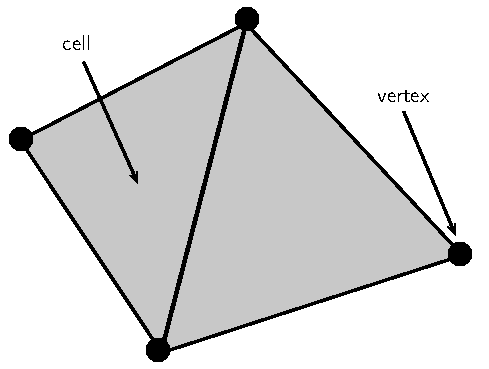
\includegraphics[width=0.4\linewidth]{./figures/eulerian/finiteElementDefinitions.pdf}
	\caption{A two-dimensional finite element geometry. The cell represents the area of the element, and vertices are the edges of the cell.}
	\label{fig:finiteElementDefinitions}
	\end{figure}

	\begin{figure}[!b]
	        \centering
	        \begin{subfigure}[b]{0.45\textwidth}
	                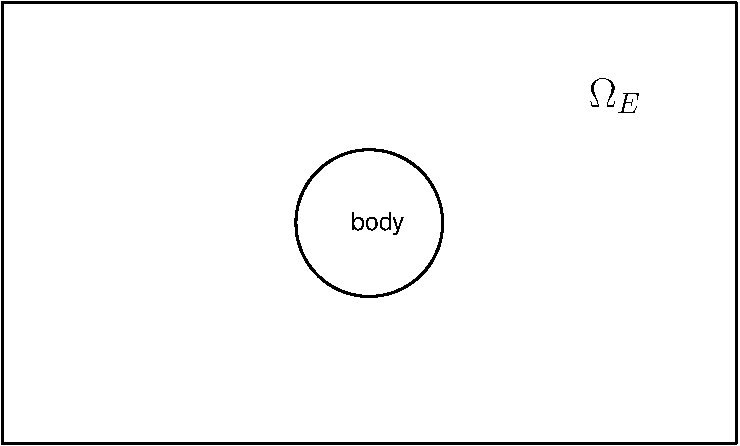
\includegraphics[width=\textwidth]{figures/eulerian/cylinderPreDelauney-crop.pdf}
	                \caption{Fluid domain $\Omega_E$ around the cylinder}
	                \label{fig:cylinderPreDelauney}
	        \end{subfigure}%
	        \qquad %add desired spacing between images, e. g. ~, \quad, \qquad etc.
	          %(or a blank line to force the subfigure onto a new line)
	        \begin{subfigure}[b]{0.45\textwidth}
	                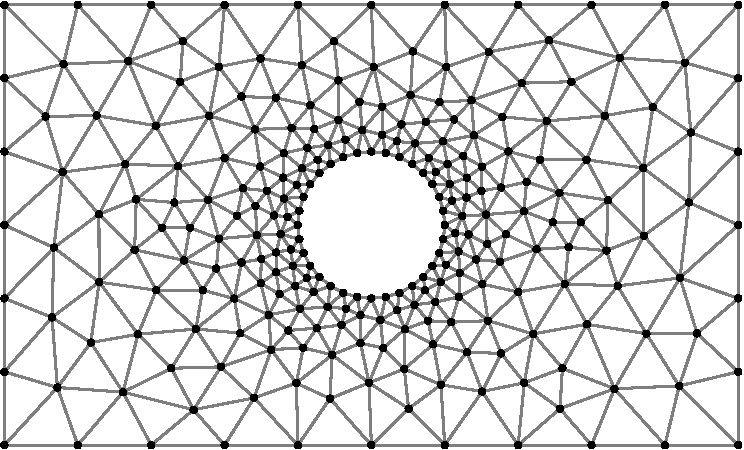
\includegraphics[width=\textwidth]{figures/eulerian/cylinderDelauney-crop.pdf}
	                \caption{Delaunay triangulation of the fluid}
	                \label{fig:cylinderDelauney}
	        \end{subfigure}
	        \caption{Delaunay triangulation of the fluid around a cylinder resulting in unstructured mesh with controllable cell sizes.}
	        \label{fig:cylinderFiniteElementDiscretization}
	\end{figure}	

A finite element discretization in 2D can be seen in Figure \ref{fig:finiteElementDefinitions}. The figure shows two connected elements, where the cells represent the area of the element, and the vertices of the cell represents the nodes of the element. The set of all the cells $\mathcal{T}_h = \{T\}$ in the fluid domain $\Omega$, constitutes the mesh of the Eulerian domain. In Figure \ref{fig:finiteElementDefinitions}, the cells of the finite element in 2D, are made of simple triangles. There are two approaches to discretize the domain: structured or unstructured meshes. The structured mesh has cells oriented in a pattern, and is the simplest approach to construct the mesh. The advantage of such a discretization is that it is possible to make a simple data structure which can be used to perform efficient computations. The downside to such discretization is that it is very difficult to construct structured mesh in complex domains with several holes. However, the FEM enables us to perform an unstructured discretization of the domain, as shown in Figure \ref{fig:cylinderFiniteElementDiscretization}. The figure shows the unstructured discretization of the fluid domain around the cylinder $\Omega_E$, connecting the rectangular outer boundary of the fluid to the circular no-slip boundary of the body in a simple fashion. Although the unstructured approach gives rise to less efficient discretization, its geometrical flexibility has advantages that surpasses the disadvantage.%This shows that even though the unstructured method formulation is more complicated that the structured formulation, we have the advantage that the mesh quality does not deteriorate as the domain becomes more complex.

There are several algorithms for mesh generation. The standard approach is to employ the Delaunay triangulation method derived from the Voronoi diagram concept \cite{Carey1997}. This divides the domain into a set of triangles, as shown in Figure \ref{fig:cylinderFiniteElementDiscretization}. This type of mesh generation allows us to connect boundaries with difference shapes together. %Furthermore, this triangulation method canbe controlled by predefining the boundary element nodes using a transfinite interpolation.

\subsection{Finite Element Functions and Function Spaces}

The finite element is defined using a triplet ($T, \mathcal{V}, \mathcal{L}$), as defined in Ciarlet \cite{Ciarlet1972b} and used in the \fenics Project \cite{Logg2012b}. $T$ is a tessellation of the domain $\Omega$, the space $\mathcal{V} = \mathcal{V}(T)$ is a finite dimensional function space on $T$ of dimension $n$, and $\mathcal{L} = \left\{ \ell_1,\ell_2,...,\ell_n \right\}$ is the set of degrees of freedom forming the basis for the dual space $\mathcal{V}'$ of $\mathcal{V}$.

Once we perform the tessellation, we can define the functions and the function spaces of the finite element problem. For each cell, a local function space $\mathcal{V}$ can be defined to collectively construct the global function space $V$. Any given function $u \in V$ is expressed as a linear combination of basis functions $\{\phi_1,\phi_2,...,\phi_N\}$,  of the function space $V$, 
	\begin{equation}
	u(x) = \sum_{j=1}^N U_j\phi_j(x).
	\end{equation}

There are several types of finite element families: the Brezzi-Douglas-Marini, the Crouzeiz-Raviart, the Discontinuous Lagrange, the Hermite, and the Lagrange elements \cite{Logg2012b}. For the current study, we will rely on the Lagrange elements, also known as the \indexAcron{Continuous Galerkin}{CG}, which are based on the Lagrange polynomials \cite{Chen2011}. These elements are widely used and are the simplest to implement for our project. 

%Each has its own advantage such as the Discontinous Lagrange, or \indexAcron{Discontinous Galerkin}{DG} element consists of discontinuous functions, which was originally introduced for solving hyperbolic problem by Reed and Hill in 1973 \cite{Reed1973a}. The method was able to conserve mass at each element, had a high-order accuracy, and was robust in solving the advection problem. However for the current problem, we will rely on the Lagrange elements, also known as the \indexAcron{Continuous Galerkin}{CG}, which are based on the Lagrange polynomials \cite{Chen2011}. These elements are widely used and are the simplest to implement for our project. 

Lagrange elements belong to the space $H^1$, which is a Sobolev space containing functions $u$ such that $u^2$ and $\left|\nabla u\right|^2$ have finite integral in the domain $\Omega$ \cite{Logg2012b}. The Lagrange element uses point evaluation for the degrees of freedom, where a DOF in $(x_i,y_i)$ denotes the point evaluation of the function $u$, $\ell_i(u) = u(x_i,y_i)$. We can have Lagrange elements of various orders $q = 1, 2,...$, where $q$ is the degree of the Lagrange polynomial $\mathcal{P}_q$. For the 2D case, the dimension $n$ of the finite element is given as,
	\begin{equation}
	n(q) = \frac{1}{2}(q + 1)(q + 2).
	\end{equation}

For $q=1$, we have a simple linear Lagrange element $\mathrm{CG}_1$ or linear interpolant with $3$ DOFs, known as the Courant triange \cite{Courant1943}. For a higher order finite element, we can set $q=2$, giving us a Lagrange element $\mathrm{CG}_2$ with $6$ DOFs per cell. Figure \ref{fig:continuousGalerkin} shows the two Lagrange triangles $\mathrm{CG}_1$ and $\mathrm{CG}_2$ for $q = 1$ and $q=2$ respectively. The Courant triangle has the DOFs located at the vertices of the cell, and the higher order $\mathrm{CG}_2$ has $3$ additional DOFs, all located midway between the vertices. Our Eulerian method of our hybrid scheme, is based on the $\mathrm{CG}_1$ and $\mathrm{CG}_2$ Lagrange elements.

	\begin{figure}[t]
	\centering
	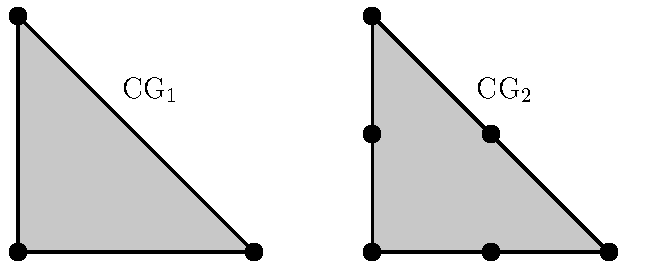
\includegraphics[width=0.6\linewidth]{./figures/eulerian/continuousGalerkin.pdf}
	\caption{The Lagrange $\mathrm{CG}_q$ triangle for $q = 1, 2$. The triangles have $3$ and $6$ DOFs respectively ({\color{black}{$\bullet$}}, black dot).}
	\label{fig:continuousGalerkin}
	\end{figure}



\subsection*{Variational Formulation}
\label{subsec:variationalProblem}

To solve a problem such as the Poisson equation numerically with FEM, we need to convert it into a variational problem. The methodology is followed from the \fenics tutorial provided by Langtangen \cite{Logg2012b}. A 1D Poisson problem is given as,
	\begin{equation}
	\begin{aligned}
	- \nabla^2 u(x) &= f(x), \qquad x\ \mathrm{in}\ \Omega,\\
	u(x) &= u_0(x), \qquad x\ \mathrm{on}\ \partial\Omega.
	\end{aligned}
	\label{eq:poissonEq}
	\end{equation}
	
We can transform equation \ref{eq:poissonEq} into a variational form by multiplying it with a test function $v$, and integrating it over the domain $\Omega$,
	\begin{equation}
	- \int_{\Omega} \left(\nabla^2 u\right)v\ \mathrm{d}x= \int_{\Omega} fv\ \mathrm{d}x, \qquad \forall\ v \in \hat{V}.
	\label{eq:poissonEqVariationFormA}
	\end{equation}

In equation \ref{eq:poissonEqVariationFormA}, the function $u$ is the trial function, and is what we are trying to approximate. The trial function $u$ lies in the trial function space $V$, and the test function $v$ lies in the test function space $\hat{V}$. When performing integration by parts, the test function $v$ is required to be zero at regions where $u$ is known. So, the additional terms cancel and we get,
	\begin{equation}
	- \int_{\Omega} \nabla u \nabla v\ \mathrm{d}x= \int_{\Omega} fv\ \mathrm{d}x \qquad \forall\ v \in \hat{V}
	\label{eq:poissonEqVariationFormB}
	\end{equation}

Equations \ref{eq:poissonEqVariationFormA} and \ref{eq:poissonEqVariationFormB} are referred to as the \textit{weak-form} of the original Poisson equation and is valid for all $v$ in the trial space $\hat{V}$. An inner product of any two functions $f$ and $g$ in domain $\Omega$ is defined as,
	\begin{equation}
	\langle f,g \rangle = \int_{\Omega}fg\ \mathrm{d}x,
	\label{eq:innerProductRule}
	\end{equation}
so we can rewrite equation \ref{eq:poissonEqVariationFormB} as,
	\begin{equation}
	-\langle \nabla u,\nabla v \rangle = \langle f,v \rangle, \qquad \forall\ v \in \hat{V}.
	\end{equation}

In order to solve this continuous problem numerically, we must transform it into a discrete variational problem,
	\begin{equation}
	-\langle \nabla u_h, \nabla v \rangle = \langle f, v \rangle \qquad \forall\ v \in \hat{V}_h \subset \hat{V},
	\label{eq:poissonEqDiscreteVariational}
	\end{equation}
where $u_h$ is the approximate solution function belonging to the discrete function in the discrete space $V_h$ which is a subset of $V$. Similarly the test discrete function space $\hat{V}_h$ is a subset of $\hat{V}$. The linear triangular element, shown in Figure \ref{fig:continuousGalerkin} is used as the function space, where $\hat{V}_h$ and $V_h$ are described by piecewise linear functions of the triangle. At the boundary, the functions in the test space are zero, whereas the functions in the trial space are equal to the boundary condition $u_0$. In the Langtangen \cite{Logg2012b}, $u$ is used to denote/write the solution of the discrete problem, ignoring the subscript $h$ of $u_h$. Therefore, to have a one-to-one relation with literature, we will employ the same notation from here on. The equation \ref{eq:poissonEqDiscreteVariational} can be simplified as,
	\begin{equation}
	a\left(u,v\right) = L(v),
	\label{eq:weakForm}
	\end{equation}
where,
	\begin{equation}
	a\left(u,v\right) = - \langle \nabla u, \nabla v \rangle,
	\end{equation}
and
	\begin{equation}
	L(v) = \langle f,v \rangle.
	\end{equation}

The variable $a(u,v)$ and $L(v)$ is the denoted as the bilinear and linear form, respectively. Since, $u\in V$, it can be written as a linear combination of the basis functions $\{\phi_i,...,\phi_N\}$ of $V$, with $\mathrm{span}\{\phi_i,...\phi_N\}=V$, we can express $u$ as,
	\begin{equation}
	u = \sum_{j=1}^{N} U_j \phi_j.
	\label{eq:trialDiscrete}
	\end{equation}
Similarly, the test function $v$ can be written as linear combination of basis functions $\{\hat{\phi}_i,...,\hat{\phi}_N\}$, with $\mathrm{span}\{\hat{\phi}_i,...,\hat{\phi}_N\}=\hat{V}$, 
	\begin{equation}
	v=\sum_{i=1}^{N} V_i \hat{\phi}_i.
	\label{eq:testDiscrete}
	\end{equation}
		
Since equation \ref{eq:weakForm} has to valid for all $v \in \hat{V}$, and $\hat{V}$ can be written as a linear combination of the basis functions, equation \ref{eq:weakForm} must be valid for each of the basis functions. Therefore, equation \ref{eq:weakForm} can be expressed as, 

	\begin{equation}
	a(\sum_{j=1}^N \ U_j \phi_j,\hat{\phi}_i) = L(\hat{\phi}_i), \qquad \forall\ \phi_i, i = 1,...,N.
	\end{equation}

and simplifies to,	
	\begin{equation}
	\sum_{j=1}^N U_j a(\phi_j,\hat{\phi}_i) = L(\hat{\phi}_i), \qquad \forall\ \phi_i, i = 1,...,N.
	\end{equation}
This is an algebraic system of equations:
	\begin{equation}
	\mathbf{A}U = b,
	\label{eq:linearSysOfEq}
	\end{equation}	
where $\mathbf{A}_{ij} = a(\phi_j,\hat{\phi}_i)$ and the \indexAcron{Right-Hand Side}{RHS} $b_i$ is given by $b_i=L(\hat{\phi}_i)$.
 	
\section{Solving the Finite Element Problem}
\label{sec:e-stfep}

To solve the finite element problem, we used \dolfin, the finite element library of the \fenics Project. This library uses high performance linear algebra kernels, and provide a scripting interface to \textsc{Python}. The Python scripting environment helps us to focus on the development of the theory (i.e the high-level algorithms). In order to generate the mesh of the fluid domain, we used \textsc{Gmsh}, a three-dimensional finite element mesh generator which proves a fast, light and user-friendly meshing tool.

\subsection{Introduction to FEniCS Project}

The \fenics Project is a collaborative work of various universities that developed tools to perform automated finite element algorithms, which can be used to solve partial differential equations. It was a project originated in 2003 with the research collaboration of University of Chicago and Chalmers University of Technology from Logg,  Mardal, and Wells \cite{Logg2012b}. Since then, several other groups have joined such as the Royal Institute of Technology, Simula Research Laboratory, University of Cambridge and Delft University of Technology.

	\begin{figure}[!h]
	\centering
	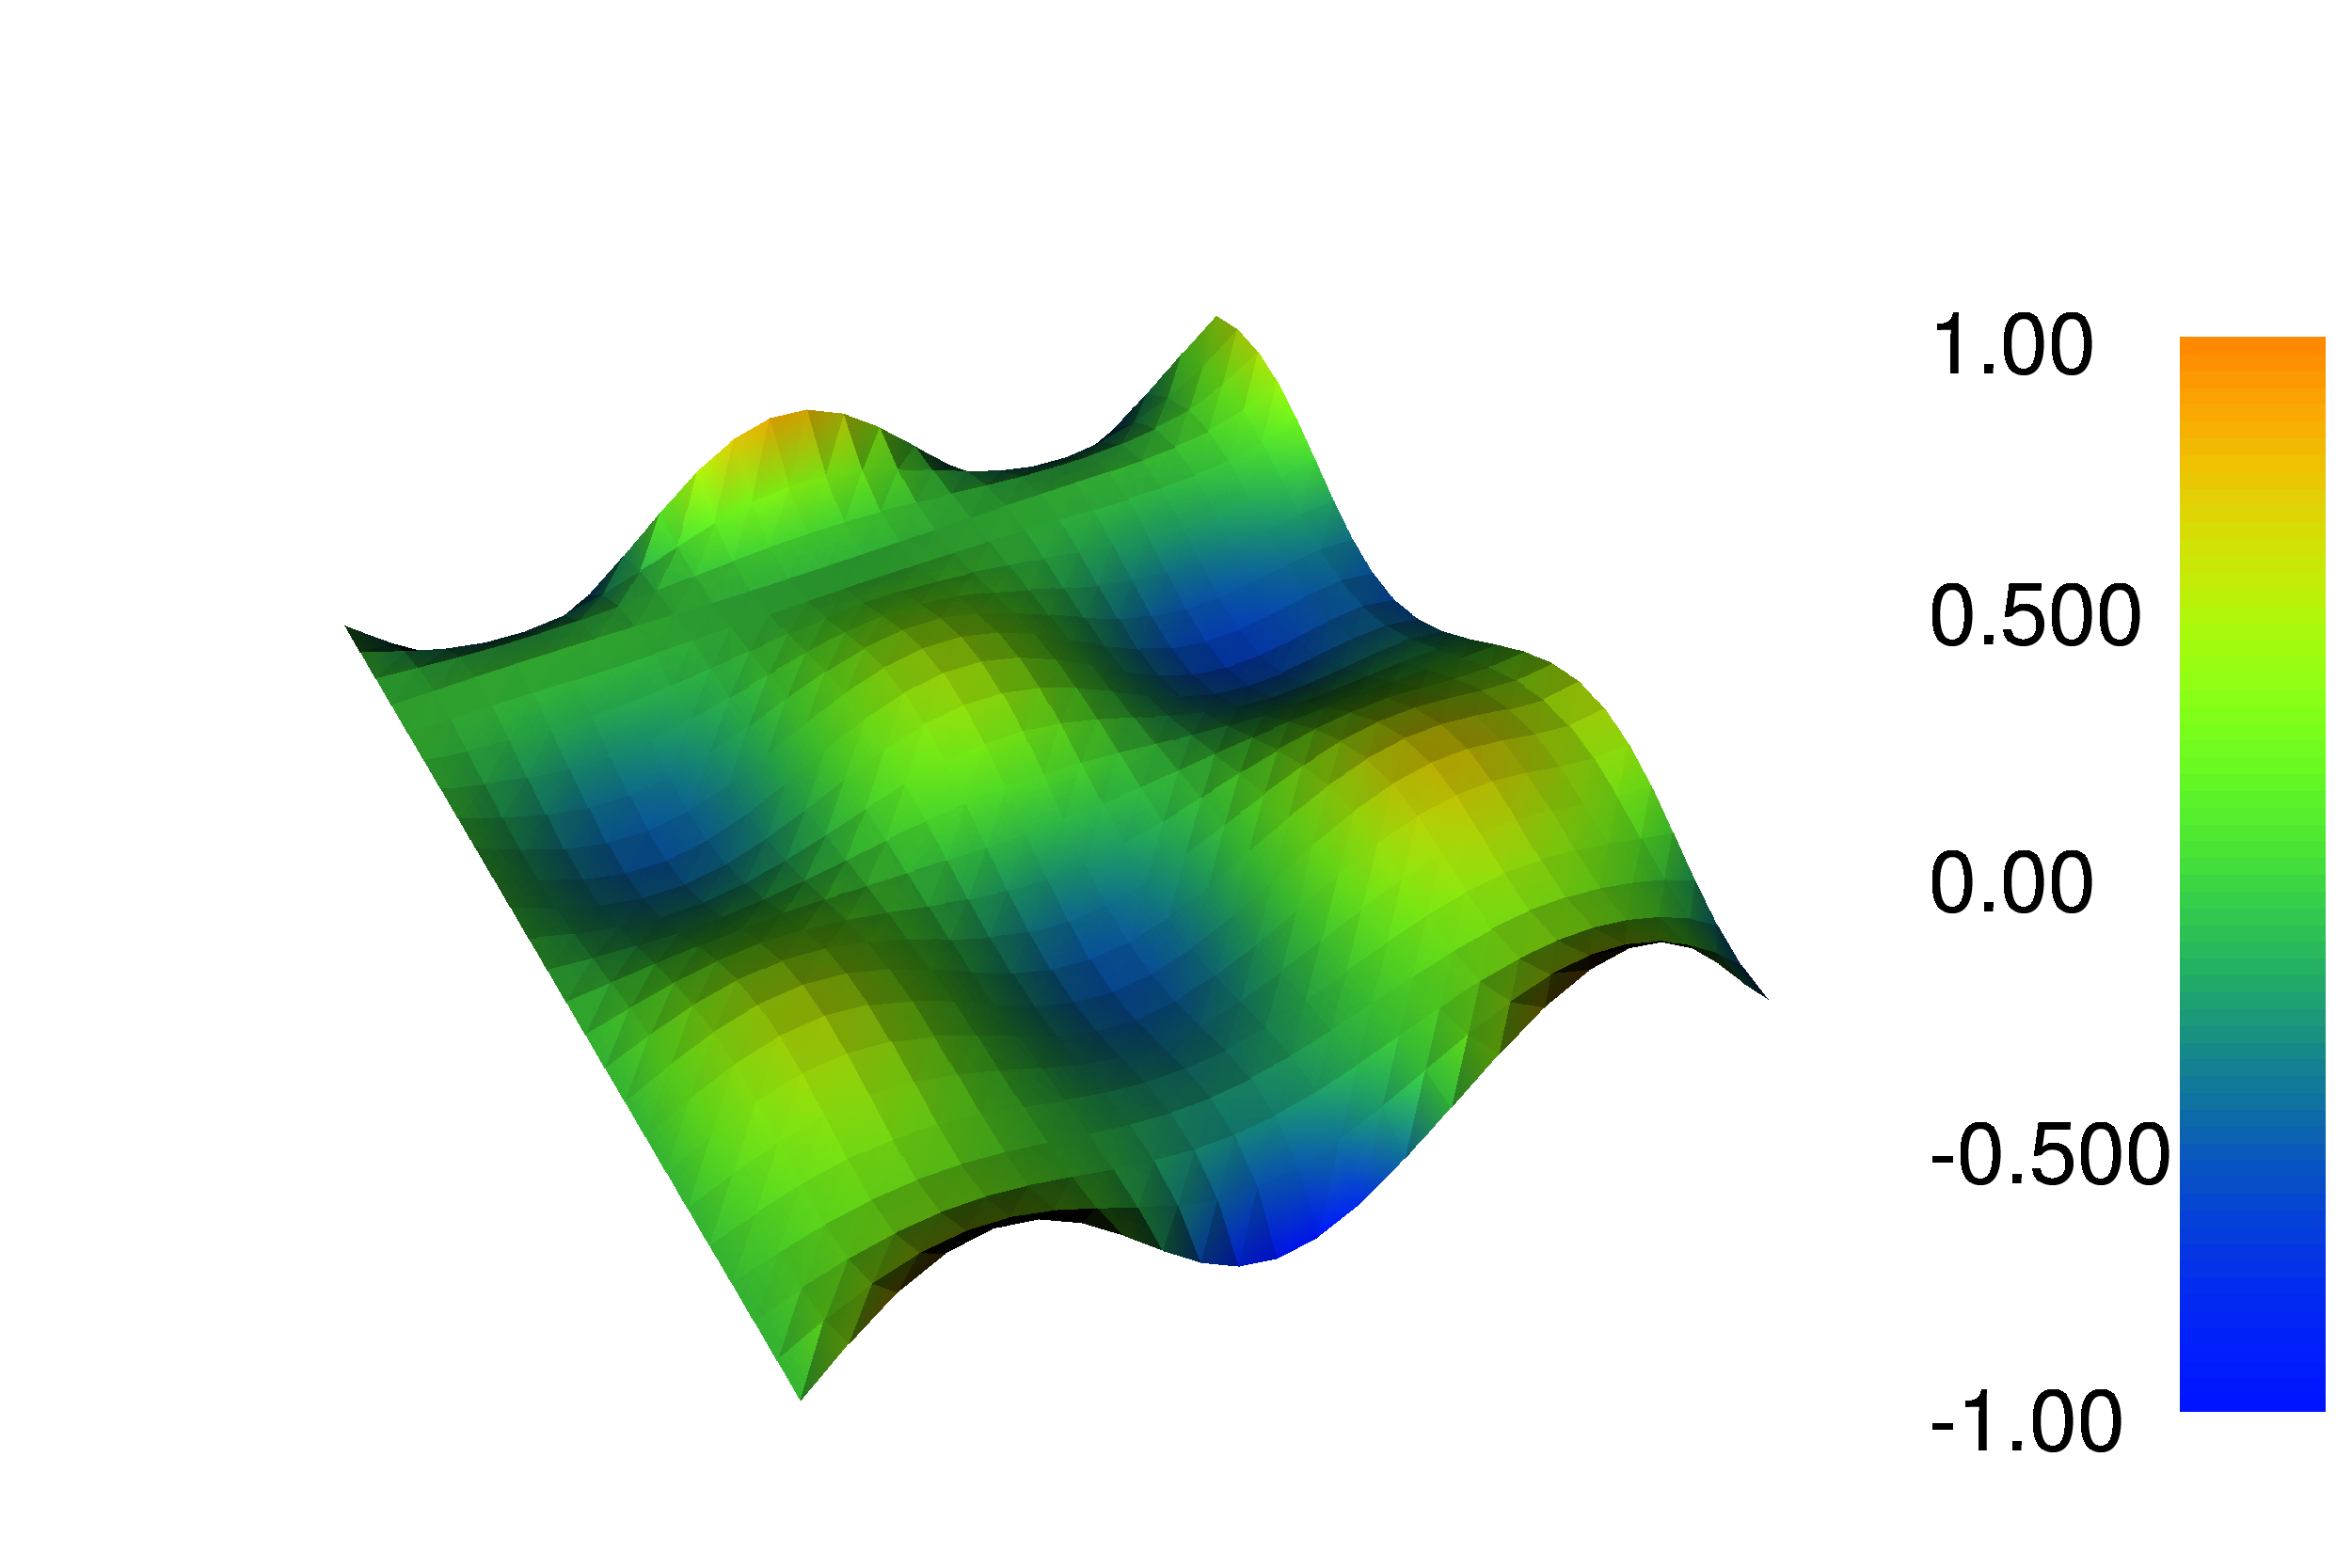
\includegraphics[width=0.5\linewidth]{./figures/eulerian/dolfin_plot_2-rotated270.png}
	\caption{\dolfin VTK plot of the Poisson solution, given by the problem, source code listing \ref{lst:pycode-poisson}.}
	\label{fig:dolfinExampleFigure}
	\end{figure}

\fenics consists of various libraries such as UFC, UFL, FIAT, INSTANT and \textsc{Dolfin}. \dolfin is the core library aimed at automating the solution of partial differential equations using the finite element method \cite{Logg2010a}. It uses automated code generation thus maintaining high-level mathematical expressions but still providing efficient, multi-threaded performance (with \indexAcron{Message Passing Interface}{MPI}) internally. %It used built-in linear algebra backend such as PETSc, TRILINOS/EPECTRA, uBLAS, and MTL4.

We used the \dolfin library wrapped in \python to set up and solve the finite element problem. For example, we can demonstrate the procedures of solving the Poisson problem, equation \ref{eq:poissonEq}. We can take $f=2\cdot\sin{x}\cdot\cos{y}$ with the boundary conditions,
	\begin{equation}
	u(x) = u_0(x) = \sin x \cdot \cos y, \qquad (x,y) \in \partial\Omega.
	\end{equation}
The finite element code generation is automated with \textsc{Dolfin}, leaving only the explicit expression of the problem in python, see source code listing \ref{lst:pycode-poisson}. Figure \ref{fig:dolfinExampleFigure} shows the VTK plot of the solution for the Poisson problem.

	\begin{listing}[p]
	\inputminted[fontseries=courier,obeytabs,fontsize=\footnotesize,mathescape,linenos,numbersep=5pt,frame=lines,framesep=2mm,xleftmargin=20mm,xrightmargin=20mm]{python}{figures/eulerian/dolfinExample.py}
	\caption{A complete program for solving the Poisson problem and plotting the solution. The Poisson problem is given as $-\nabla^2{u} = f$, where $u_0 = \sin{x}\cdot\cos{y}$ on the boundary and $f=2\cdot\sin(x)\cdot\cos(y)$. The code is written in \python using \dolfin 1.2 library}
	\label{lst:pycode-poisson}
	\end{listing}

\subsection{Mesh Generation using GMSH}
\label{subsec:mgugmsh}
%The proper generation of the fluid mesh is an important aspect of the Finite Element method. It is an important process, as an ill-construct mesh can be computationally very expensive, or might even problem with convergence. There have been literatures dedicated just to improve the mesh generation, for example by Hansen \cite{Hansen2005}. It focused on mesh enhancement techniques for elliptical methods, which enables to increase the quality of the data, and also the robustness of the simulation.

The generation of the mesh is achieved by \textsc{Gmsh}, an open-source software developed by Geuzaine \& Remacle \cite{Geuzaine2009b}, which has implemented a user-friendly interface and fast algorithms. The \gmsh implemented kernels use \textsc{BLAS} and LAPACK linear algebra packages in C++ for fast computation. Furthermore, it allows for scriptability making it ideal to integrate it with our current \python code project for future automation.

\section{Solving Incompressible Navier-Stokes Equations}
\label{sec:e-sinse}

Using the \dolfin library for constructing the finite element problem, we can now solve the flow in the Eulerian subdomain of our hybrid scheme. The Eulerian method use the primitive variables velocity-pressure $\mathbf{u}-p$ to describe the flow.

\subsection{Velocity-Pressure Formulation}
The velocity-pressure $\mathbf{u}-p$ formulation of the fluid flow problem, is the standard formulation of the Navier-Stokes equations. The 2D incompressible Navier-Stokes equations of a fluid with unit density (i.e $\rho = 1$) is given as,
	\begin{subequations}
	\begin{align}
	\frac{\partial \mathbf{u}}{\partial t} + \mathbf{u}\cdot\nabla\mathbf{u} - \nabla \cdot \sigma &= f,\\
	\nabla \cdot \mathbf{u} = 0,
	\end{align}	
	\label{eq:2Dns}
	\end{subequations}
where $\sigma$ is the Cauchy stress tensor defined as,
	\begin{equation}
	\sigma(\mathbf{u},p) = 2\nu\epsilon(\mathbf{u}) - p\mathbf{I}.
	\label{eq:stressTensor}
	\end{equation}

The Cauchy stress tensor is a function of pressure $p$, the fluid kinematic viscosity $\nu$, and the symmetric gradient $\epsilon$ defined as,
	\begin{equation}
	\epsilon(\mathbf{u}) = \frac{1}{2} \left(\nabla \mathbf{u} + \nabla \mathbf{u}^{\mathrm{T}}\right).
	\label{eq:symGrad}
	\end{equation}
describing the stresses in the fluid due to the velocity gradient and the pressure. The incompressible 2D Navier-Stokes equations have two unknowns, the vector velocity field $\mathbf{u}$, that lies on the vector-valued function space $V$, and the scalar pressure field $p$, which lies on the scalar-valued function space $Q$. Once we compute these two quantities we can determine the vorticity field, which we then transfer to the Lagrangian subdomain. 

\subsection{Determining the Vorticity Field}
\label{subsec:dtvf}

The coupling between the Eulerian and the Lagrangian subdomain is done by transferring the vorticity field $\omega$ from the Eulerian subdomain to the Lagrangian vortex blobs. The vorticity field $\omega$, is defined as:
	\begin{equation}
	\omega = \nabla \times u,
	\label{eq:vorticityEq}
	\end{equation}
where the vorticity $\omega$ lies on the scalar-valued function space $X$. However, as $\nabla\times\mathbf{u}\notin{X}$, because $\mathbf{u}\in V$, we require a projection from the velocity function space $V$ onto the vorticity function space $X$. In weak form, this requires the following equality to be satisfied,
%Due to the constant change in the velocity field, we have to recalculate the vorticity at every time step $t_n, t_{n+1}, ...$ . To solve this problem in an efficient manner, we can use the \texttt{assemble} function of \dolfin to pre-construct the problem. %We must first define the equation \ref{eq:vorticityEq} in the variational (integral) form,  
	\begin{equation}
	\int_{\Omega} \omega \cdot v\ \mathrm{d}x = \int_{\Omega} (\nabla \times \mathbf{u}) \cdot v\ \mathrm{d}x, \qquad \forall\ v \in \hat{X}.
	\label{eq:variationalFormulationofVorticity}
	\end{equation}
To determine the vorticity at every step of the simulation $t_n, t_{n+1}, ...$, we have to perform this projection at every step. Thus, to solve this problem in an efficient manner, we can pre-assemble (i.e pre-calculated) the knowns of the problem using the \texttt{assemble} function of \dolfin. 

Using the inner product rule, defined by equation \ref{eq:innerProductRule}, equation \ref{eq:variationalFormulationofVorticity} can be rewritten as,
	\begin{equation}
	-\langle \nabla \omega,\nabla v \rangle = \langle \nabla \times \mathbf{u},v \rangle, \qquad \forall\ v \in \hat{X}.
	\label{eq:variationalFormulationofVorticityInProduct}
	\end{equation}
where $\hat{X}$ is the test function space of the trial function space $X$. Equation 	\ref{eq:variationalFormulationofVorticityInProduct} can also be written as, 
		\begin{equation}
		a(\omega,v) = L(\mathbf{u},v), \qquad \forall\ v \in \hat{X},
		\label{eq:variationalFormulationofVorticityInProductSimple}
		\end{equation}
where $a(\omega,v) = -\langle \nabla \omega,\nabla v \rangle$, and $L(\mathbf{u},v) =  \langle \nabla \times \mathbf{u},v \rangle$. Since $\omega$ can be written as a linear combination of basis functions $\{\psi_j,...,\psi_N\}$, with $\mathrm{span}\{\psi_j,...,\psi_N\} = X$, we can express $\omega$ as,
		\begin{equation}
		\omega = \sum_{j=1}^N w_j\psi_j,
		\label{eq:vorticityLinear}
		\end{equation}
Similarly, $v$ and $\mathbf{u}$ can be expressed in the linear form as $v = \sum_{i=1}^N V_i \hat{\psi}_i$ and $\mathbf{u} = \sum_{j=1}^N U_j \phi_j$, respectively. 

As described in section \ref{subsec:variationalProblem}, since equation \ref{eq:variationalFormulationofVorticityInProductSimple} is valid for all $v \in \hat{X}$, and as $\hat{X}$ can be written as a linear combination of basis functions $\{\hat{\psi}_i,...,\hat{\psi}_N\}$, equation \ref{eq:variationalFormulationofVorticityInProductSimple} must be valid for each of the basis functions.  Therefore, equation \ref{eq:variationalFormulationofVorticityInProductSimple} can be expresses in the linear form as, 
		\begin{equation}
		a(\sum_{j=1}^N w_j\psi_j,\hat{\psi}_i) = L(\sum_{i=j}^N U_j \phi_j,\hat{\psi}_i), \qquad \forall\ \hat{\psi}_i,\ i=1,...N,
		\label{eq:variationalFormulationofVorticityInProductSimpleLinear}
		\end{equation}
and simplifying to,
		\begin{equation}
		\sum_{j=1}^N w_j\cdot{a}(\psi_j,\hat{\psi}_i) = \sum_{i=j}^N U_j\cdot{L}(\phi_j,\hat{\psi}_i), \qquad \forall\ \hat{\psi}_i,\ i=1,...N,
		\label{eq:variationalFormulationofVorticityInProductSimpleLinearSum}
		\end{equation}
resulting in an algebraic system of equations,
		\begin{equation}
		\mathbf{A}w = b,
		\label{eq:variationalFormulationofVorticityInProductSimpleLinearSumSoE}
		\end{equation}
where $\mathbf{A}_{ij} = a(\psi_j, \hat{\psi}_i)$, and the \printAcron{Right-Hand-Side}{RHS} is given as $b_i = L(\phi_i, \hat{\psi_i})$. Since $\mathbf{A}$ does not change during the simulation, it can be pre-computed outside the time-marching loop, using the \texttt{assemble} function of \dolfin, improving the efficiency of the vorticity calculation.

	\begin{listing}[!t]
	\inputminted[fontseries=courier,obeytabs,fontsize=\footnotesize,mathescape,linenos,numbersep=5pt,frame=lines,framesep=2mm,xleftmargin=20mm,xrightmargin=20mm]{python}{figures/eulerian/vorticity.py}
	\caption{The \textsc{python} implementation of the vorticity calculation using \dolfin 1.2 library. Line 24 shows the use of \texttt{assemble} function to pre-assemble the knowns of the problem.}
	\label{lst:pycode-vorticity}
	\end{listing}

The \textsc{python} implementation of the algorithm is show in listing \ref{lst:pycode-vorticity}. Using the \dolfin library, we can used the \texttt{assemble} function to pre-calculated the LHS of the problem (line 24). So using the algorithms of the hybrid coupling scheme, we can transfer this vorticity field of the Eulerian subdomain on the vortex blobs.

%Using the approach described in section \ref{subsec:variationalProblem}, equation \ref{eq:variationalFormulationofVorticityInProductSimple} can be simplifying to an algebraic system of equations:
%	\begin{equation}
%	\mathbf{A}w = b
%	\end{equation}
%where $\mathbf{A}_{ij}$ is the coefficient matrix, $w = [\hat{\omega}_j,...,\omega_N]^{\mathrm{T}}$ and $b$ is given by $b_i=L(\hat{\phi}_i)$.
\subsection{Taylor-Hood Finite Element Family for Solving ICNS}
To solve the \indexAcron{Incompressible Navier-Stokes}{ICNS} problem, we must choose appropriate finite element function spaces for the velocity $\mathbf{u}$ and the pressure $p$ by ensuring that we satisfy the Ladyzhenskaya-Babu\v{s}ka-Brezzi (LBB) compatibility condition, also known as the inf-sup compatibility condition, described in Brezzi and Fortin \cite{Brezzi1991}. The Lagrange finite element space for velocity must be one order higher than the order of the pressure $q_{\mathrm{pres}}$,
	\begin{equation}
	q_{\mathrm{vel}} = 	q_{\mathrm{pres}} + 1,
	\end{equation}
for a stable formulation. Therefore, we have decided to use the Taylor-Hood family, introduced by Taylor and Hood \cite{Taylor1973} and verified by Boffi \cite{Boffi1997}, that satisfies the inf-sup compatibility condition by using $q_{\mathrm{vel}} = 2$ and $q_{\mathrm{pres}} = 1$. We decided to choose this method, as it is the most conventional method, that is simple, and shows a stable behavior.

%Brezzi and Fortin \cite{Brezzi1991} showed that if both have the same order, it will result in an unstable problem. To solve the ICNS problem, we will used the Taylor-Hood family \cite{Taylor1973}, examined by Boffi \cite{Boffi1997}. The method use velocity order $q_{\mathrm{vel}} = 2$ and pressure order $q_{\mathrm{pres}} = 1$. We decided to choose this method, as it is the most conventional method, that is simple, and that shows a stable behavior.

In addition, we have to choose an appropriate function space for the vorticity. As vorticity is the curl of the velocity, to reduce interpolation error during the projection of the solution, we will use a function space one order lower than the velocity, $q_{\mathrm{vort}} = 1$. Table \ref{tab:eulerianFunctionTerms} shows the list of the function spaces, the finite element type and their orders. Additionally, we have included the variable names of the function space, trial functions and the test functions, associated to the function element that we have chosen for the problem.

	\ctable[
	    caption = {Summary of the Lagrange element $\mathrm{CG}_q$ of order $q$, that was used for solving the incompressible Navier-Stokes problem. The variable names of the function space, the trial functions, and the test functions are tabulated together.},
	    label   = {tab:eulerianFunctionTerms},
	    pos = h,
	]{lcccc}{}{\FL
	Variable	& Finite element & Function space	& Trial function & Test function \ML
	Velocity	& $\mathrm{CG}_2$	& $V$			& $\mathbf{u}$	 & $\mathbf{v}$\\
	Pressure 	& $\mathrm{CG}_1$ 	& $Q$			& $p$	 		 & $q$\\
	Vorticity 	& $\mathrm{CG}_1$	& $X$			& $w$	 		 & $x$\LL}


\subsection{Incremental Pressure Correction Scheme}
\label{subsec:ipcs}
This algorithm to solve the NS problem was first demonstrated by Chorin in 1968 \cite{Chorin1968}, and is referred to as Chorin's projection method or sometimes known as the non-incremental pressure correction scheme. The process relies in first computing a tentative velocity by initially neglecting the pressure in the momentum equation of the Navier-Stokes problem, equation \ref{eq:2Dns}. The velocity field is corrected by determining the pressure field satisfying a divergence free vector field. This method however does not satisfy the discrete incompressibility constraint exactly and so, Goda in 1979 \cite{Goda1979a}, introduced an improved \indexAcron{Incremental Pressure Correction Scheme}{IPCS}. The method computed the viscous term at the incremented time $(t_{n-1} + t_n)/2$, and used the stress formulation to determine the corrected pressure \cite{Logg2012b}. The detailed algorithms to the IPCS scheme, as presented in the \fenics manual \cite{Logg2012b}, can be summarized as follows:

	\begin{enumerate}
	\item \textbf{Compute the tentative velocity:} The tentative velocity $\mathbf{u}^{\star}$ is determined by solving,
		\begin{equation}
		\begin{split}
		\langle D_t^n \mathbf{u}^{\star}, \mathbf{v} \rangle &+ \langle \mathbf{u}^{n-1}\cdot\nabla\mathbf{u}^{n-1},\mathbf{v}\rangle + \langle \sigma(\mathbf{u}^{n-\frac{1}{2}},p^{n-1}), \epsilon(\mathbf{v}) \rangle \quad \\ &\quad+ \langle p^{n-1}\hat{\mathbf{n}},\mathbf{v}\rangle_{\partial \Omega} - \langle \mathbf{v}\ \hat{\mathbf{n}} \cdot (\nabla \mathbf{u}^{n-\frac{1}{2}} )^{\mathrm{T}},\mathbf{v} \rangle_{\partial \Omega} = \langle f^n,\mathbf{v} \rangle,
		\end{split}
		\label{eq:tentativeVel}
		\end{equation}
	is valid for all $\mathbf{v} \in V$, where $\mathbf{u}^{n-\frac{1}{2}}$ is defined as,
		\begin{equation}
		\mathbf{u}^{n-\frac{1}{2}} = \frac{\mathbf{u}^{\star}+\mathbf{u}^{n-1}}{2},
		\end{equation}
	With the Dirichlet velocity boundary conditions at the boundary $\partial \Omega$, we can solve equation \ref{eq:tentativeVel}. The additional term,
		\begin{equation}
		\langle \mathbf{v}\ \hat{\mathbf{n}} \cdot (\nabla \mathbf{u}^{n-\frac{1}{2}} )^{\mathrm{T}},\mathbf{v} \rangle_{\partial \Omega},
		\end{equation}
	is results from integration by parts, when we evaluate the viscous term at $(t_{n-1} + t_n)/2$ and we use the stress formulation instead of the Laplacian formulation as done for the Chorin scheme. This difference ensures that the velocity profile at the inlet and the outlet of the domain is more accurate that the ones obtained for the Chorin scheme. 
	
		\begin{listing}[!t]
		\inputminted[fontseries=courier,obeytabs,fontsize=\scriptsize,mathescape,linenos,numbersep=5pt,frame=lines,framesep=2mm,xleftmargin=20mm,xrightmargin=20mm]{python}{figures/eulerian/tentativeVelocity.py}
		\caption{The source code for solving the tentative velocity $\mathbf{u}^{\star}$, using the equation \ref{eq:tentativeVel}.}
		\label{lst:pycode-tentativeVelocity}
		\end{listing}	
	
	The source code for solving the tentative velocity problem is shown in listing \ref{lst:pycode-tentativeVelocity}. First, we pre-define all the terms needed for the tentative velocity problem formulation (lines \numrange{3}{16}). We can also pre-assemble the LHS of the problem (line 19) outside of the time-integration loop, since it remains constant. During time integration, we first assemble the RHS of the problem (line 26), then apply the Dirichlet velocity boundary condition (line 29) which consists of the wall boundary condition, and external Dirichlet velocity boundary condition (e.g. the free-stream). Finally, we can solve the problem using a GMRES solver for solving the system of linear equation (line 32).
	
	\item \textbf{Determine the pressure:} The pressure $p^n$ is determined by solving,	
		\begin{equation}
		\langle \nabla p^n, \nabla q \rangle = \langle \nabla p^{n-1}, \nabla q\rangle - \langle \nabla \cdot \mathbf{u}^{\star}, q \rangle / \Delta t_n
		\label{eq:pressureCorrection}
		\end{equation}
	valid for all $q \in Q$. We use the previously calculated tentative velocity $\mathbf{u}^{\star}$ to determine the pressure. We can solve the problem using the Neumann pressure boundary condition at the pressure outlet of the domain. We define a boundary as the pressure outlet, if we do not know the velocity boundary condition at that boundary. This is true for the region where the exit flow is perturbed. However, for the coupled Eulerian method (that we will use), all the boundary conditions are available as a velocity boundary condition from the Lagrangian subdomain. This means that we do not have to assume any pressure boundary condition.

		\begin{listing}[!t]
		\inputminted[fontseries=courier,obeytabs,fontsize=\scriptsize,mathescape,linenos,numbersep=5pt,frame=lines,framesep=2mm,xleftmargin=20mm,xrightmargin=20mm]{python}{figures/eulerian/correctedPressure.py}
		\caption{The source code for solving the pressure $p^n$ using the equation \ref{eq:pressureCorrection}.}
		\label{lst:pycode-correctedPressure}
		\end{listing}

	The source code for solving the pressure problem is shown in listing \ref{lst:pycode-correctedPressure}. As done for the tentative velocity, we can formulate and pre-assemble the problem before the time loop (lines \numrange{3}{9}). In the time loop, we only need to assemble the RHS (line 16), apply the boundary condition (if it exists, lines \numrange{18}{20}) and finally solve for the pressure (lines \numrange{22}{24}). Using the pressure, we can determine the corrected velocity field. 
		
	\item \textbf{Determine the corrected velocity:} The corrected velocity field $u^n$ is determined by solving,
		\begin{equation}
		\langle \mathbf{u}^n, \mathbf{v}\rangle = \langle \mathbf{u}^{\star},\mathbf{v} \rangle - \Delta t_n \langle \nabla(p^n - p^{n-1}),\mathbf{v} \rangle,
		\label{eq:velocityCorrection}	
		\end{equation}
	which is valid for all $\mathbf{v} \in V$. We correct the tentative velocity $\mathbf{u}^{\star}$ by the pressure difference to determine the correct velocity field. We will have to apply the Dirichlet velocity boundary condition at the boundary again, to solve for the problem.
	
		\begin{listing}[!t]
		\inputminted[fontseries=courier,obeytabs,fontsize=\scriptsize,mathescape,linenos,numbersep=5pt,frame=lines,framesep=2mm,xleftmargin=20mm,xrightmargin=20mm]{python}{figures/eulerian/correctedVelocity.py}
		\caption{The source code for solving the corrected velocity $u^n$ using equation 		\ref{eq:velocityCorrection}.}
		\label{lst:pycode-correctedVelocity}
		\end{listing}	
	
	The source code for solving the corrected velocity problem in shown in listing \ref{lst:pycode-correctedVelocity}. We first initialize the problem, by formulating the problem and assembling the LHS outside the time loop (line \numrange{3}{8}). In the time integration loop, we assemble the RHS (line 15), apply the velocity boundary condition (line 18) and finally solve for the corrected velocity field (line 21).

	\end{enumerate}
	
The algebraic system of equations resulting form this algorithm have been solved with \textsc{Dolfin}'s Krylov \textsc{Gmres} solver with an absolute and a relative error tolerance of \num{e-25} and \num{e-12} respectively. The program structure was based on the collection of benchmark solvers provided by the \fenics \cite{nsbench}. In the  algorithm described above an explicit time marching scheme, \printAcron{Forward Euler}{FE} has been used. Therefore, for the time marching scheme to be stable, we require the CFL number to satisfy the following condition:
	\begin{equation}
	\mathrm{CFL} = \Delta t_{E,\mathrm{max}} \frac{\lVert\mathbf{u}\rVert_{\mathrm{max}}(\nu +  \Delta h_{\mathrm{min}}\lVert\mathbf{u}\rVert_{\mathrm{max}})}{\Delta h_{\mathrm{min}}^2} \leqslant 1.
	\label{eq:cfl}
	\end{equation}
	
This gives us the direct constraint on the maximum Eulerian time step size $\Delta t_{E,\mathrm{max}}$ which is function of the $\mathrm{CFL}$ number, maximum fluid velocity in the Eulerian domain $\lVert \mathbf{u} \rVert_{\mathrm{max}}$, the fluid viscosity $\nu$ and the minimum mesh cell size $\Delta h_{min}$. 

%When coupling with the Lagrangian method, we will see that $\Delta t_E \leqslant \Delta t_L$ (Lagrangian time step size is ideally larger than Eulerian time step size), meaning that we will have to perform $k_E$ Eulerian sub-steps to reach the Lagrangian step, figure \ref{fig:multiStep}.

\subsection{Determining the Body Forces}

After we determine the flow fields, we can compute the lift and the drag generated by the body. To determine these parameters, we first need to determine the forces acting on the no-slip boundary, which can be determined from the stress tensor $\sigma$ acting on the surface of the body, equation \ref{eq:stressTensor}. The lift coefficient and the drag coefficient are computed by:
	\begin{subequations}
	\begin{align}
	L &= \int_{\partial \Omega} \left[\sigma(\mathbf{u},p) \cdot \hat{\mathbf{n}}\right]\cdot \hat{\mathbf{e}}_y\ \mathrm{d}s,\\
	D &= \int_{\partial \Omega} \left[\sigma(\mathbf{u},p) \cdot \hat{\mathbf{n}}\right]\cdot \hat{\mathbf{e}}_x\ \mathrm{d}s,
	\end{align}
	\label{eq:LiftDragEq}
	\end{subequations}
where $\hat{\mathbf{e}}_x$ and $\hat{\mathbf{e}}_y$ are the 2D unit Cartesian vectors,
	\begin{equation}
	\hat{\mathbf{e}}_x = \begin{bmatrix}
	 1 \\ 
	 0 
	\end{bmatrix}, \qquad \quad 
	\hat{\mathbf{e}}_y = \begin{bmatrix}
		 0 \\ 
		 1 
		\end{bmatrix}.\\
	\end{equation}

such that lift perpendicular to the free-steam and the drag is tangential to it. The lift coefficient $C_l$ and the drag coefficient $C_d$, are obtained by normalizing the lift $L$ and drag $D$ forces with the dynamics pressure and reference length $c$ (in 2D), where the lift perpendicular to the free-steam and the drag is tangential to it,
		\begin{equation}
		C_l = \frac{L}{\frac{1}{2}\lVert\mathbf{u}\rVert_{\infty}^2 c},\qquad \quad
		C_d = \frac{D}{\frac{1}{2}\lVert\mathbf{u}\rVert_{\infty}^2 c}.\\
		\label{eq:LiftDragCoeffEq}
		\end{equation}


	\begin{listing}[!h]
	\inputminted[fontseries=courier,obeytabs,fontsize=\footnotesize,mathescape,linenos,numbersep=5pt,frame=lines,framesep=2mm,xleftmargin=20mm,xrightmargin=20mm]{python}{figures/eulerian/forces.py}
	\caption{The \textsc{python} implementation for calculating the lift force $L$ and the drag force $D$ acting on the no-slip boundary.}
	\label{lst:pycode-forceCalculation}
	\end{listing}

%. The stress tensor $\sigma$ is given by,
%	\begin{equation}
%	\sigma(\mathbf{u},p) = 2\nu\epsilon(\mathbf{u}) - p\mathbf{I},
%	\end{equation}
%where $\epsilon$ is the symmetric gradient, equation \ref{eq:symGrad}, and is a function of the velocity $\mathbf{u}$ and the pressure $p$ acting on the surface.

\section{Evolution of the Eulerian Method}
\label{sec:eu-eotem}
The algorithm of evolving the Eulerian method is summarized in this section. The Eulerian method acts as the source of the vorticity for the Lagrangian method.

	\begin{figure}[!h]
		\centering
		\begin{tikzpicture}
			[node distance=.8cm, start chain=going below,]
			\node[punktchainN, join] (meshGen) {\textsf{Generation Eulerian mesh}};
		    \node[punktchainN, join] (bc) {\textsf{Determine boundary conditions}};
		    \node[punktchainN, join] (solve)     {\textsf{Solve the IPCS}};
		    \node[punktchainN, join] (vort) 	  {\textsf{Determine the vorticity}};
		\end{tikzpicture}
		\caption{Flowchart of the Eulerian method.}
		\label{fig:flowchart_eulerian}
	\end{figure}	
	
The flowchart of the Eulerian method is given by Figure \ref{fig:flowchart_eulerian}.The algorithm to the Eulerian method can be summarized as follows:
	\begin{enumerate}
	\item \textbf{Mesh generation}: We generate the mesh of the fluid domain using \gmsh before the iteration.
	\item \textbf{Determine the boundary condition}: We determine the boundary conditions for the boundary domains: $\partial \Omega_E = \Sigma_{w} \cup \Sigma_{d}$. The Dirichlet velocity boundary condition is obtained directly the Lagrangian method and the Neumann pressure boundary condition is obtained from the velocity. This is possible as we known the complete velocity distribution at all $\partial \Omega_E$. 
	
%	If we have Dirichlet velocity boundary conditions for all the exterior boundaries, we do not have to apply any pressure boundary conditions at $\partial \Sigma_{p}$, because $\Sigma_{p}=\emptyset$ in that case.
	\item \textbf{Solve the IPCS}: Using IPCS, time march from $t_n$ to $t_{n+1}$ to solve for the new velocity $\mathbf{u}$ and pressure $p$ field.
	\item \textbf{Determine the vorticity}: Using the algorithm described in \ref{subsec:dtvf}, solve for the vorticity field $\omega$ at the time $t_{n+1}$. 
	\end{enumerate}
	
Once we have the well-resolved vorticity $\omega$ of the near-body region, the vorticity is then transfered into the Lagrangian subdomain using the Hybrid coupling scheme, which was summarized in chapter \ref{ch:helvpm}, and fully elaborated in chapter \ref{ch:coupling}.

\section{Validation of Eulerian Method}
\label{sec:eu-voem}

To verify our Eulerian method, we first investigated the Lamb-Oseen vortex problem. The validation of the Eulerian method is done by investigating the Clercx-Bruneau dipole collision at $Re=625$, comparing with the study of Clercx and Bruneau \cite{Clercx2006a}. Furthermore, we investigated the problem of the impulsively started cylinder at $Re=550$, where we verified and validated the lift and drag calculations with the literature of Koumoutsakos and Leonard \cite{Koumoutsakos1995a}, and Rosenfeld et al. \cite{MosheRosenFeldDochanKwak1991}.

\subsection{Lamb-Oseen Vortex}
\label{subsec:eulerianLambOseen}

The Lamb-Oseen vortex is an analytical solution by Lamb and Oseen, describing the diffusion of a vortex core \cite{Tryggeson2007}. The current investigation was performed similarly to the Lagrangian study in section \ref{subsec:lagrangianLambOseen}. 
%We solved the same problem as the one described in the Lagrangian validation problem \ref{subsec:lagrangianLambOseen}. 

\subsubsection*{Problem Definition}

%In the Lagrangian method, the Lamb-Oseen vortex was initialized using the vorticity field as the vortex blobs carry circulation strengths. However, Eulerian domain use the primitive variables $\mathbf{u}-p$ for formulating the problem. Therefore, we use the Lamb-Oseen velocity field as the initial conditions for the problem. 
%	\ctable[
%		caption = {Summary of the parameters for the Lamb-Oseen vortex evolution.},
%		label   = {tab:eulerianLambOseenParams},
%		pos = !b,]{lcll}{}{\FL
%		
%		Parameters 					& Value 	& Unit					& Description \ML
%		$\Gamma_c$\T               	& 1 &\si{m^2.s^{-1}} 				& Core strength\\
%		$\Omega$               		& $\left[-1,1\right]\times \left[-1,1\right]$ &\si{m}		& Eulerian domain bounds \\
%		$\mathbf{u}_{\infty}$ 		& $0$ &\si{m.s^{-1}} & Free-stream velocity\\
%		$\nu$						& $\num{5e-4}$ &\si{kg.s^{-1}.m^{-1}}& Kinematic viscosity\\
%			$ \tau$ 		    & 4 &\si{s}	& Lamb-Oseen time constant\\
%		$ t$ 		    	& \numrange{0}{1} &\si{s}			& Simulation time span\\		
%		$ \Delta t$ 				& $0.001$ &\si{s}					& Time step size\\
%		$ N_{\mathrm{t-steps}}$ 	& 1000 & -							& Number of time integration steps\\		
%		$ h_{\mathrm{min}}$			& $\frac{1}{100}\sqrt{2}$ &\si{m}	& Minimum mesh cell size\\	        
%		$ N_{\mathrm{cells}}$ 		& $200^2$ 	& -						& Number of mesh cells\\
%		$ \mathrm{CFL}$								& $0.95$ & -		& CFL number\\	        	        
%		$\lVert \mathbf{u} \rVert_{\mathrm{max}}$	& $1.5$	& 	\si{m.s^{-1}} & Maximum magnitude fo the velocity\\	
%		Time integration & FE & - & Forward Euler time integration method\LL}

	\ctable[
		caption = {Summary of the parameters for the Lamb-Oseen vortex evolution.},
		label   = {tab:eulerianLambOseenParams},
		pos = !b,]{lcll}{}{\FL
		
		Parameters 					& Value 	   & Description \ML
		$\Gamma_c$\T               	& 1 			& Core strength\\
		$\Omega$               		& $\left[-1,1\right]\times \left[-1,1\right]$ 	& Eulerian domain bounds \\
		$\mathbf{u}_{\infty}$ 		& $0$ & Free-stream velocity\\
		$\nu$						& $\num{5e-4}$ & Kinematic viscosity\\
			$ \tau$ 		    & 4 & Lamb-Oseen time offset\\
		$ t$ 		    	& \numrange{0}{1} 			& Simulation time span\\		
		$ \Delta t$ 				& $0.001$ 				& Time step size\\
		$ N_{t}$ 	& 1000 					& Number of time integration steps\\		
		$ h_{grid}$			& $\approxeq0.01$   & Minimum mesh cell size\\	        
		$ N_{cells}$ 		& $161312$ 					& Number of mesh cells\\
		$ \mathrm{CFL}$								& $0.95$ 	& CFL number\\	        	        
		$\lVert \mathbf{u} \rVert_{\mathrm{max}}$	& $1.5$	& 	Maximum magnitude of the velocity\\	
		Time integration & FE & Forward Euler time integration method\LL}

In section \ref{subsec:lagrangianLambOseen}, the vortex blobs of the Lagrangian method required the vorticity formulation of the Lamb-Oseen vortex to set up the problem. However, as the Eulerian method use the primitive variables $\mathbf{u}-p$, we require the velocity formulation of the Lamb-Oseen vortex. The velocity field of the Lamb-Oseen vortex is defined as,
	\begin{subequations}
	\begin{align}
	u_{\theta} &= \frac{\Gamma_c}{2\pi r} \left[1-\exp\left(-\frac{r^2}{4\pi\nu(t+\tau)}\right)\right]\\
	u_r &= 0,
	\end{align}
	\label{eq:eLO_veq}
	\end{subequations}	
where $u_{\theta}$ is the circumferential velocity, and $u_r$ is the radial velocity. The velocity is a function of the vortex core strength $\Gamma_c$, the simulation time $t\in[0,\infty[$, the time constant $\tau$, the kinematic viscosity $\nu$, and the distance from the core center $r$.

The parameters used for the simulation are tabulated in Table \ref{tab:eulerianLambOseenParams}. To ensure a valid comparison of the present Eulerian method study with the Lagrangian method performed in section \ref{subsec:lagrangianLambOseen}, we chose similar spatial discretization parameters.

	\begin{figure}[!t]
	\centering
	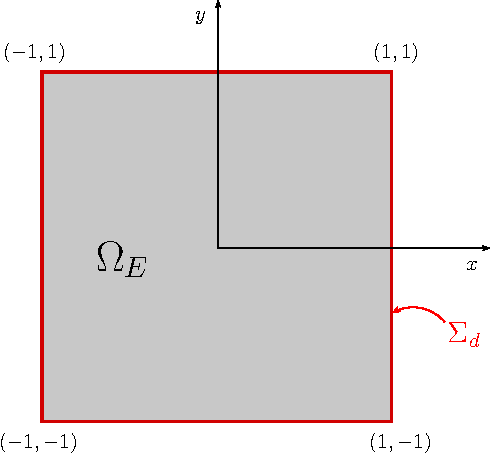
\includegraphics[width=0.5\linewidth]{./figures/eulerian/lambOseenDomainDefinition-crop.pdf}
	\caption{Eulerian domain $\Omega_E$ ({\color{plotGray}{\textbf{gray}}}) for the Lamb-Oseen vortex problem, bounded by the Dirichlet velocity boundary $\Sigma_d$ ({\color{plotRed}{\textbf{red}}}), where the Dirichlet velocity boundary condition was applied. The parameters of the domain are tabulated in Table \ref{tab:eulerianLambOseenParams}.}
	\label{fig:lambOseenDomainDefinition}
	\end{figure}

Figure \ref{fig:lambOseenDomainDefinition} depicts the domain for the present Lamb-Oseen vortex study. The fluid domain $\Omega_E$ is bounded by a Dirichlet boundary $\Sigma_d$ such that $\partial \Omega_E = Sigma_d$. The Dirichlet boundary $\Sigma_d$ is used to prescribe the analytical Dirichlet velocity boundary conditions for the Lamb-Oseen vortex problem.
 
The Eulerian method is time marched using the time integration parameters tabulated in Table \ref{tab:eulerianLambOseenParams}. To ensure a stable time integration, we enforced the CFL conditions, equation \ref{eq:cfl}. During the evolution of the solution, we evaluated the growth of the error in velocity, and the error in vorticity between the numerical and the analytical solutions.

%where $\Gamma_c$ is the vortex core strength, $\tau \equiv \nu t$ is the scaled viscous time, and $r$ is the distance from the core center. The parameters of the simulation is tabulated in table \ref{tab:eulerianLambOseenParams}. To ease the comparison of the Eulerian to the Lagrangian method, we performed ensure similar spatial resolution. The figure \ref{fig:lambOseenDomainDefinition} shows the domain of the problem, discretized the domain $\Omega = \left[-1,1\right]^2$ in a structure grid with the number of finite element cells $N_{\mathrm{cells}}=200^2$ in $x$ and $y$ direction, minimum cell size $h=\sqrt{2}/100$. 



%Furthermore, the figure \ref{fig:lambOseenDomainDefinition} also shows the boundary domains $\partial \Omega$ of the fluid domain. For the Lamb-Oseen problem, as we have the analytical solution of the velocity field for all time, we can use this solution to prescribe the external domain boundary condition. So for this problem, we only need an external Dirichlet velocity boundary condition, at the boundary domain identified as, $\mathrm{ID}_{\mathrm{ext}} = 3$. This would imply that we do not need to explicitly apply the pressure boundary condition, as we already have a velocity boundary condition. With all the boundary conditions, we can evolve the initial velocity distribution of the Lamb-Oseen vortex from $t_0 = 4$ to $t_f =5$, using the IPCS algorithm described in section \ref{subsec:ipcs}. 

%	\begin{figure}[p]
%	\centering
%	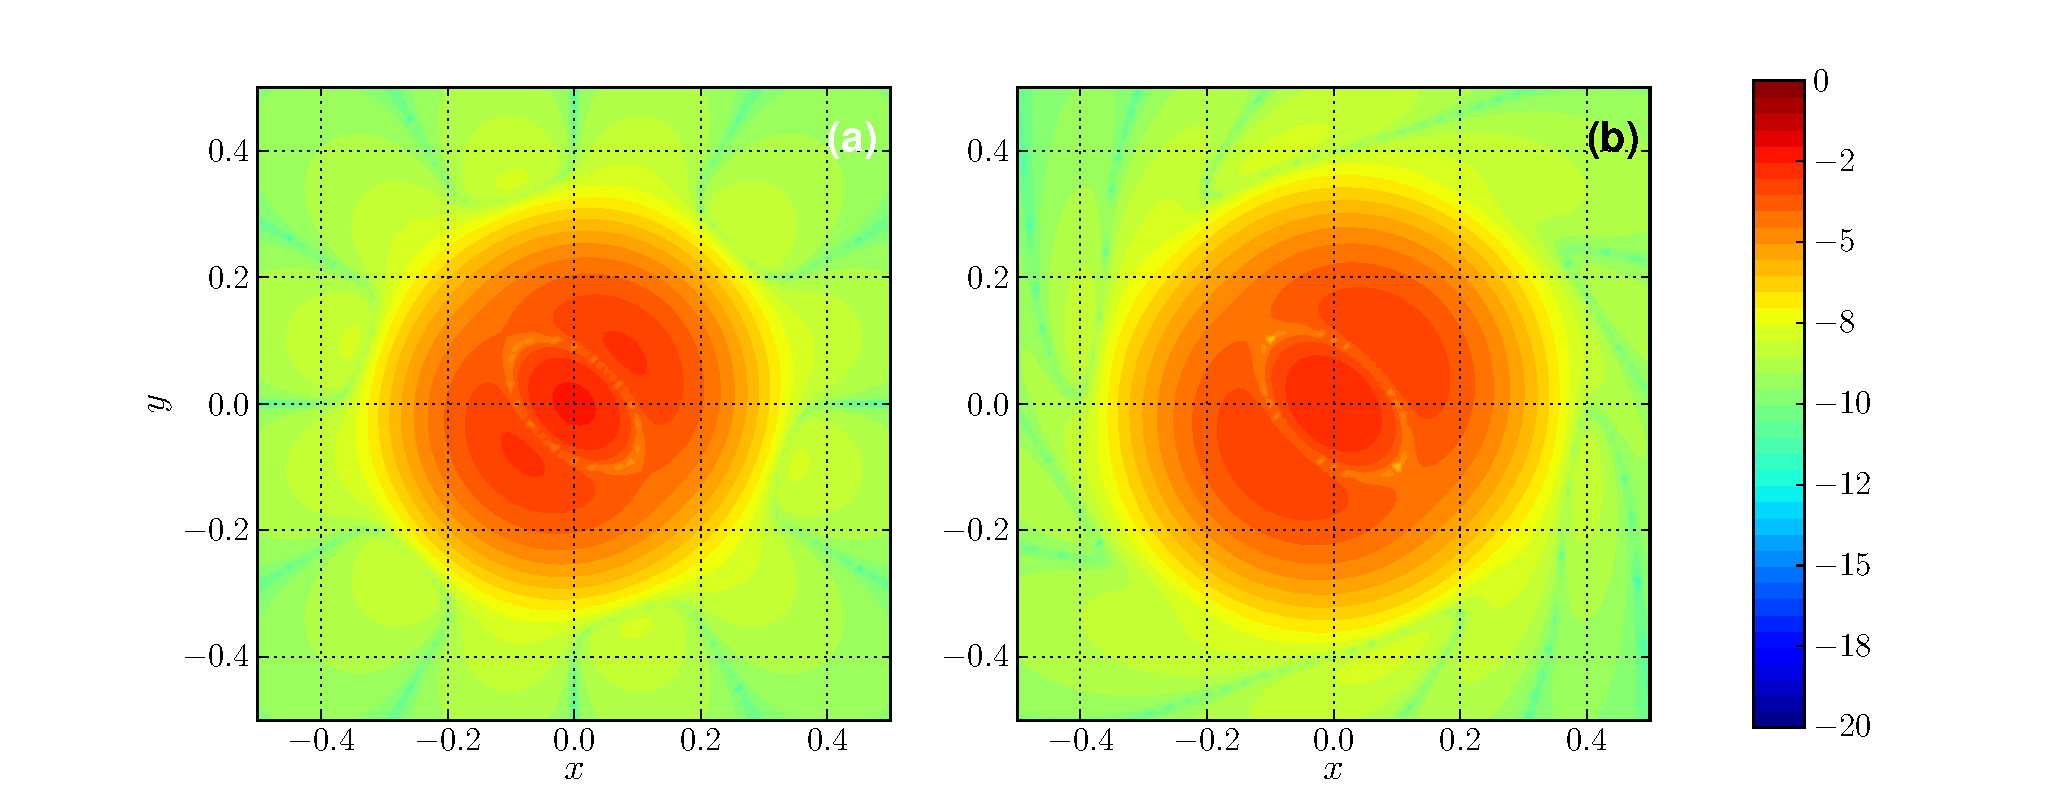
\includegraphics[width=0.99\linewidth]{./figures/eulerian/lambOseen_eulerian_wRelField_compressed.pdf}
%	\caption{Relative error in vorticity field in logarithmic scale. Figure \textbf{(a)} shows the initial relative error in vorticity at $t=0$, and figure \textbf{(b)} shows the relative error in vorticity at the end of the time stepping $t=1$. The parameters of the simulation are tabulated in table \ref{tab:eulerianLambOseenParams}.}
%	\label{fig:lambOseen_eulerian_wRelField_compressed}
%	\end{figure}
	
	\begin{figure}[p]
     \centering
     \begin{subfigure}[b]{0.45\textwidth}
             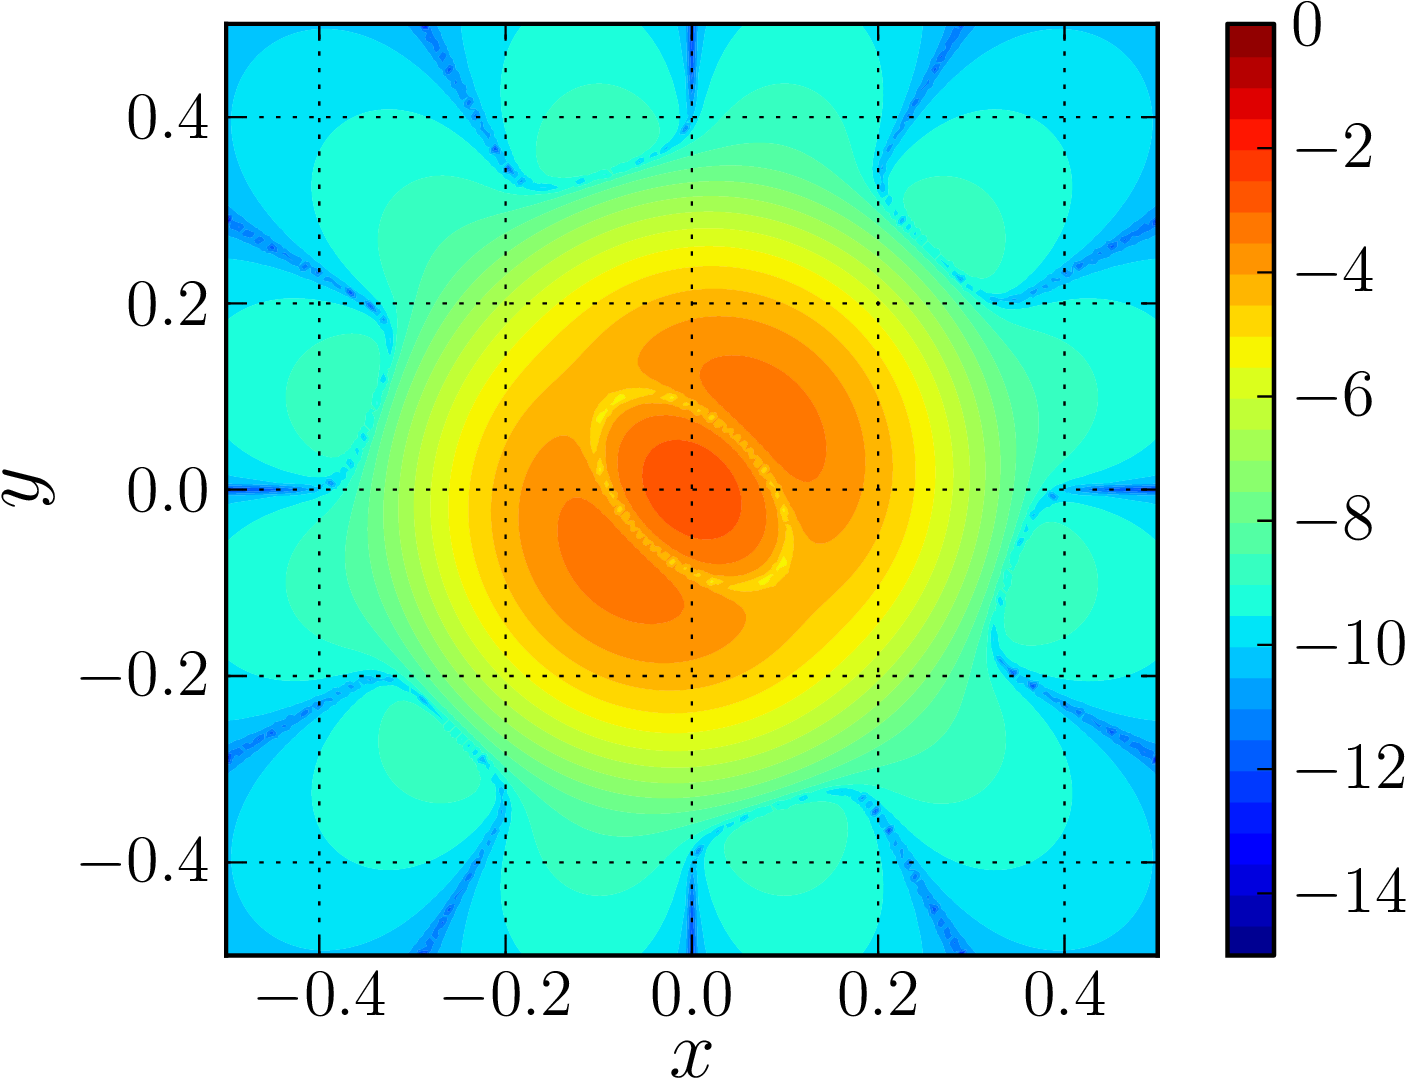
\includegraphics[width=\textwidth]{figures/eulerian/lambOseen_wErrorInitial_compressed-crop.png}
             \caption{$t=0$}
             \label{fig:lambOseen_wErrorInitial_compressed-crop}
     \end{subfigure}%
     \qquad %add desired spacing between images, e. g. ~, \quad, \qquad etc.
       %(or a blank line to force the subfigure onto a new line)
     \begin{subfigure}[b]{0.45\textwidth}
             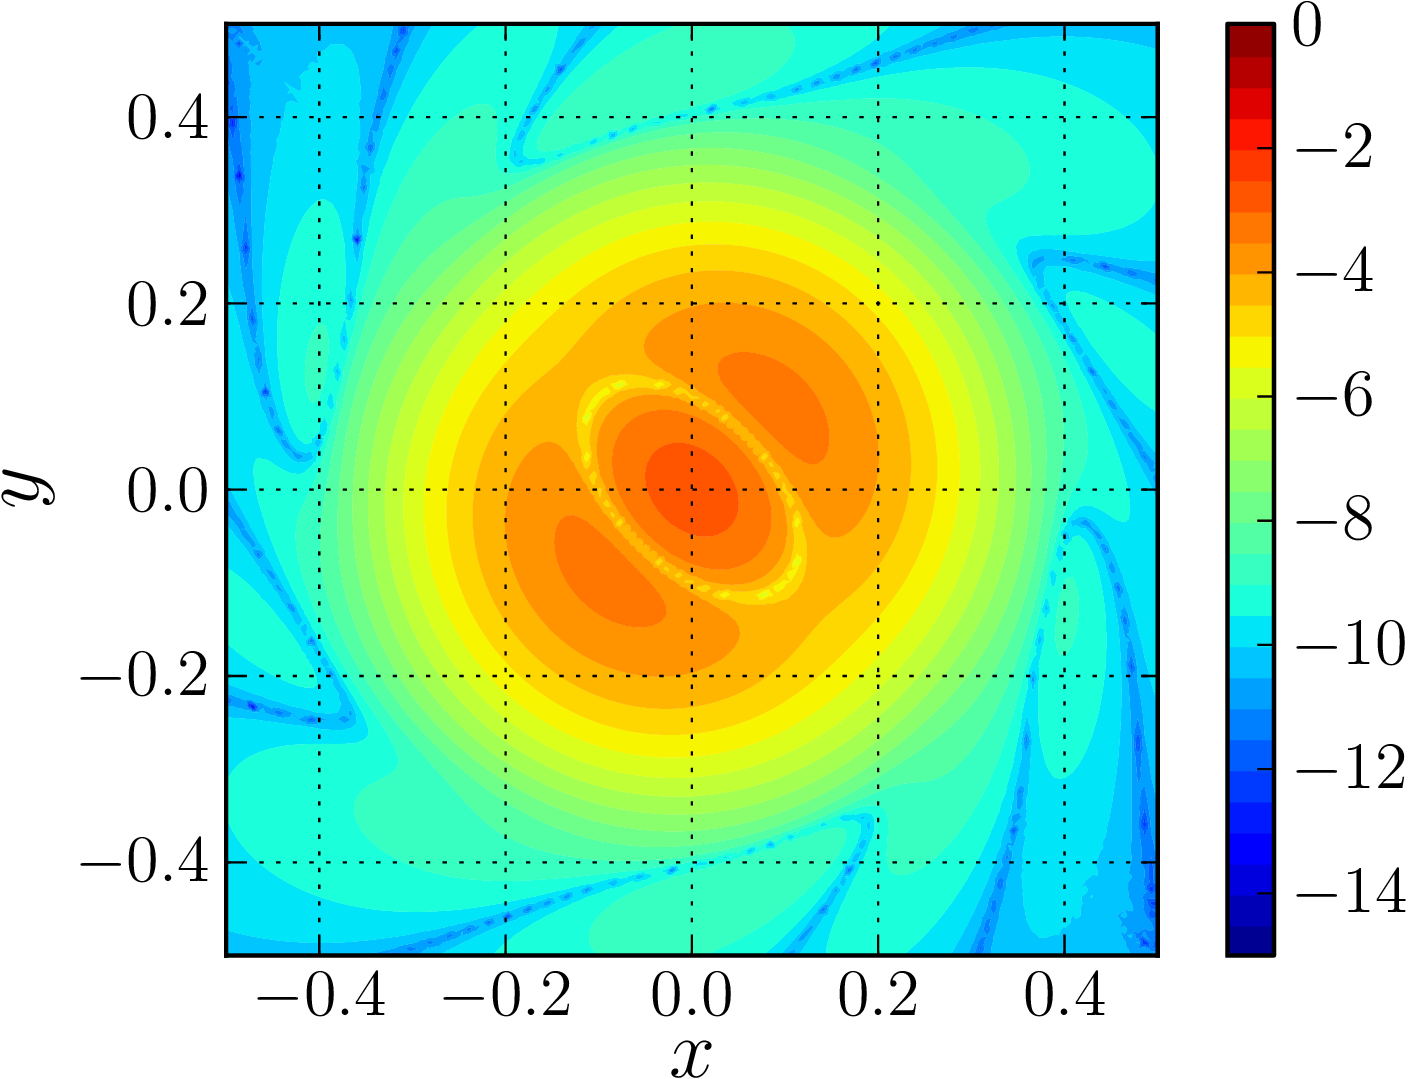
\includegraphics[width=\textwidth]{figures/eulerian/lambOseen_wErrorFinal_compressed-crop.png}
             \caption{$t=1$}
             \label{fig:lambOseen_wErrorFinal_compressed-crop}
     \end{subfigure}
     
     \caption{Relative error in vorticity (in logarithmic scale) using the parameters tabulated in Table \ref{tab:eulerianLambOseenParams}. The figure shows \textbf{(a)}, the initial relative error in vorticity at $t=0$, and \textbf{(b)} the final relative error in vorticity at $t=1$.}
     \label{fig:lambOseen_eulerian_wRelField_compressed}
	\end{figure}	
	
	\begin{figure}[p]
	\centering
	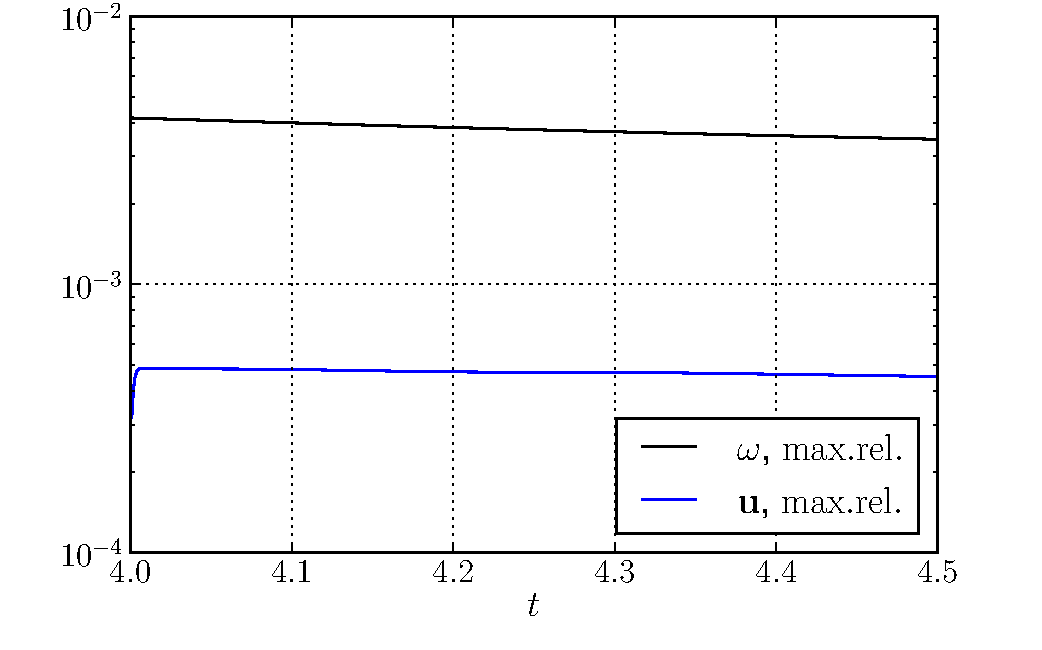
\includegraphics[width=0.6\linewidth]{./figures/eulerian/lambOseen_eulerian_wRelEvolution_compressed.pdf}
	\caption{Evolution of the maximum relative errors from $t=0$ to $t=1$ using the parameters in Table \ref{tab:eulerianLambOseenParams}. The figure depicts maximum relative error in velocity [{\color{plotBlue}{---}}, solid {\color{plotBlue}{\textbf{blue}}}] and the maximum relative error in vorticity [---, solid \textbf{black}]. }
	\label{fig:lambOseen_eulerian_wRelEvolution}
	\end{figure}


	\begin{figure}[p]
        \centering
        \begin{subfigure}[b]{0.5\textwidth}
                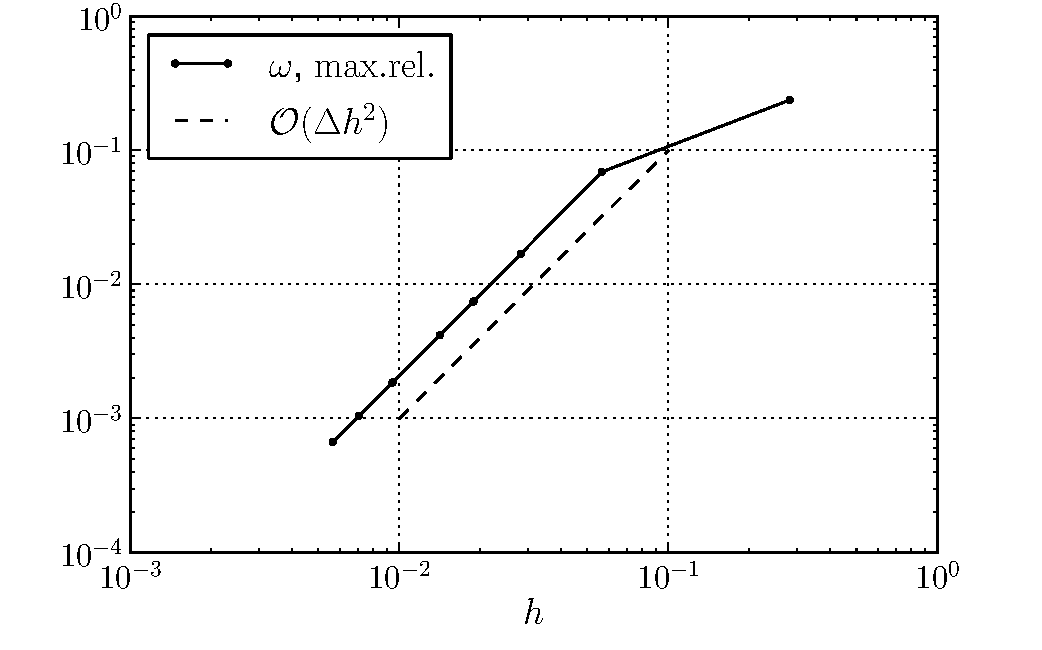
\includegraphics[width=\textwidth]{figures/eulerian/lambOseen_eulerianConvergence_dx_compressed.pdf}
                \caption{Spatial convergence}
                \label{fig:lambOseen_eulerianConvergence_dx}
        \end{subfigure}%
        ~ %add desired spacing between images, e. g. ~, \quad, \qquad etc.
          %(or a blank line to force the subfigure onto a new line)
        \begin{subfigure}[b]{0.5\textwidth}
                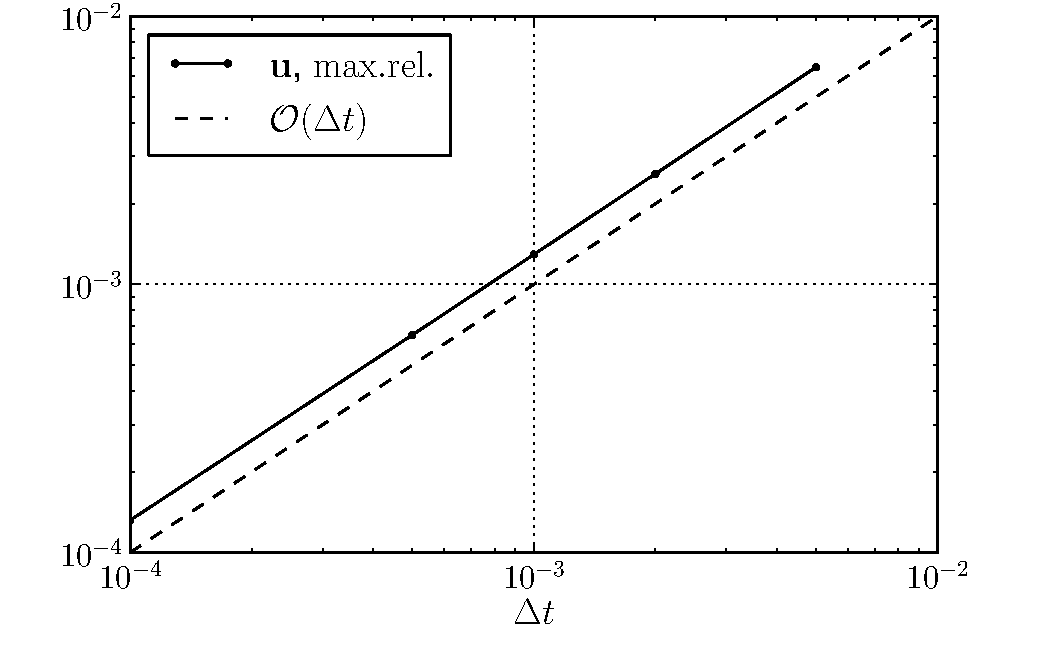
\includegraphics[width=\textwidth]{figures/eulerian/lambOseen_eulerianConvergence_dt_compressed.pdf}
                \caption{Temporal convergence}
                \label{fig:lambOseen_eulerianConvergence_dt}
        \end{subfigure}
        \caption{Convergence in space and time. The figure depicts \textbf{(a)} convergence in space of $\mathcal{O}(\Delta h^2)$ and \textbf{(b)} convergence in time of $\mathcal{O}(\Delta t)$. The control parameters are tabulated in Table \ref{tab:eulerianLambOseenParams}.}
        \label{fig:lambOseen_eulerianConvergence}
	\end{figure}		
	

%We used $CFL$ stability condition equation \ref{eq:cfl}, to determine the time step size, $\Delta t = 0.001$. The Eulerian method time steps using a \printAcron{Forward Euler}{FE} time marching and requires $N_{\mathrm{t-steps}}=1000$ time steps. During the evolution, we evaluated the growth of the error in velocity, and in vorticity between the numerical results and the analytical solution. 

\subsubsection*{Results and Discussion}

We are interested in the evolution of error in vorticity, as this is the quantity which will be interpolated onto the Lagrangian subdomain. Figure \ref{fig:lambOseen_eulerian_wRelField_compressed} shows the initial and the final relative error in vorticity over the Eulerian domain. Opposed to the Lagrangian results, Figure \ref{fig:lambOseen_convection_vorticityErrorContours}, we see that initial relative error in the vorticity field is larger. This is so because the Eulerian solution was initialized using the velocity and the vorticity is obtained by projecting $\nabla\times\mathbf{u}$ (see section \ref{subsec:dtvf}
) onto the scalar-valued function space $W$, whereas the Lagrangian solution was initialized directly from vorticity. This process of initialization in the Eulerian domain introduces additional numerical error in the vorticity. However, the pattern of the relative error in vorticity is similar to the Lagrangian solution, with the highest error at the core center, where we have stronger vorticity.

As time progresses, we see that the error in the solution does not increase as observed for the Lagrangian method, Figure \ref{fig:lambOseen_eulerian_wRelField_compressed}b. Figure \ref{fig:lambOseen_eulerian_wRelEvolution} shows this change in the maximum relative error in velocity and vorticity. The maximum relative error in vorticity is at all times higher than the maximum relative error in velocity, due to the error in projection.

To determine the convergence with spatial resolution, the simulation was run for $h \approx 0.25$ to $h \approx \num{5e-3}$. Figure \ref{fig:lambOseen_eulerianConvergence_dx} shows the convergence of the relative error in vorticity. This validates that the scheme is $2^{\mathrm{nd}}$-order in space, which is expectable due to the second order function space $\mathrm{CG}_2$ for the primitive variable, velocity.

To determine convergence with time resolution, we ran the simulation with various time steps $\Delta t = \num{5e-3}$ to $\Delta t = \num{1e-4}$. As we performed the investigation, we saw that the error in the primitive variable $\mathbf{u}$, converged with order 1, Figure \ref{fig:lambOseen_eulerianConvergence}. This is expected, as have employed a $1^{\mathrm{st}}$-order Forward Euler scheme. Thus, we have verified against the analytical solution of the Lamb-Oseen vortex that our Eulerian method is well implemented and performs in a robust manner.

\subsection{Clercx-Bruneau Dipole Collision at $Re=625$}
\label{subsec:eul_cbdc}
The Eulerian method that we have developed here is to be used as a wall-bounded Eulerian solver that can resolve the vorticity production at the boundary for the Hybrid method. Therefore it is vital that the vortex interaction with the no-slip boundary is handled properly.

To determine the proper handling of the no-slip boundary, it is common practice to use a simple test of dipole colliding with the wall. In these test cases, one could observe how the no-slip boundary handles the incoming vortex and can be used to determine if the system is formulated appropriately.  Ould-Salihi et al. \cite{Ould-Salihi2001a} used this case to validate their Hybrid method that couples vortex particles with finite-difference method. Cottet et al. \cite{Cottet2000b} used this test case to validate the vortex method. Therefore in a similar fashion, we have decided to use the dipole collision study by Clercx and Bruneau \cite{Clercx2006a}, performed using a Chevyshev pseudo-spectral method, to verify and validate our Eulerian method. 

%Therefore, we decided to use the Clercx-Bruneau dipole collision is a test case from Clercx \& Bruneau \cite{Clercx2006a}, where they performed a numerical study of a normal collision of a dipole with a no-slip boundary. This experiment provide extensive benchmark results for various Reynolds numbers with a Chevyshev pseudo-spectral numerical method. 

\subsubsection*{Problem Definition}

Unlike other dipole test cases, Clercx and Bruneau provide well-defined initial and boundary conditions for the dipole vorticity field. Furthermore, they used a vorticity distribution that was continuous, which ensures a smooth velocity field for our Eulerian method using the $\mathbf{u}-p$ formulation. The literature provided results for the collision that we are interested: a normal collision with the dipole traveling perpendicular to the wall.

	\begin{figure}[!b]
     \centering
     \begin{subfigure}[t]{0.45\textwidth}
             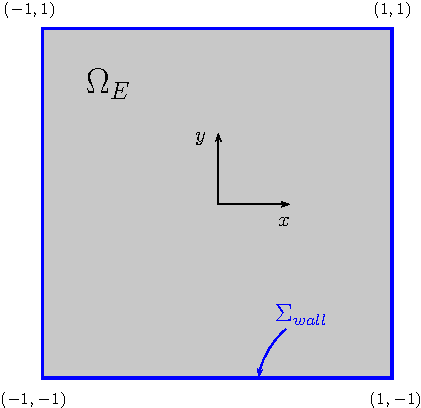
\includegraphics[width=\textwidth]{figures/eulerian/clercxBruneauDomainDefinition-crop.pdf}
             \caption{(\textit{Not to scale}) Domain definition}
             \label{fig:clercxBruneauDomainDefinition}
     \end{subfigure}%
     \qquad %add desired spacing between images, e. g. ~, \quad, \qquad etc.
       %(or a blank line to force the subfigure onto a new line)
     \begin{subfigure}[t]{0.45\textwidth}
             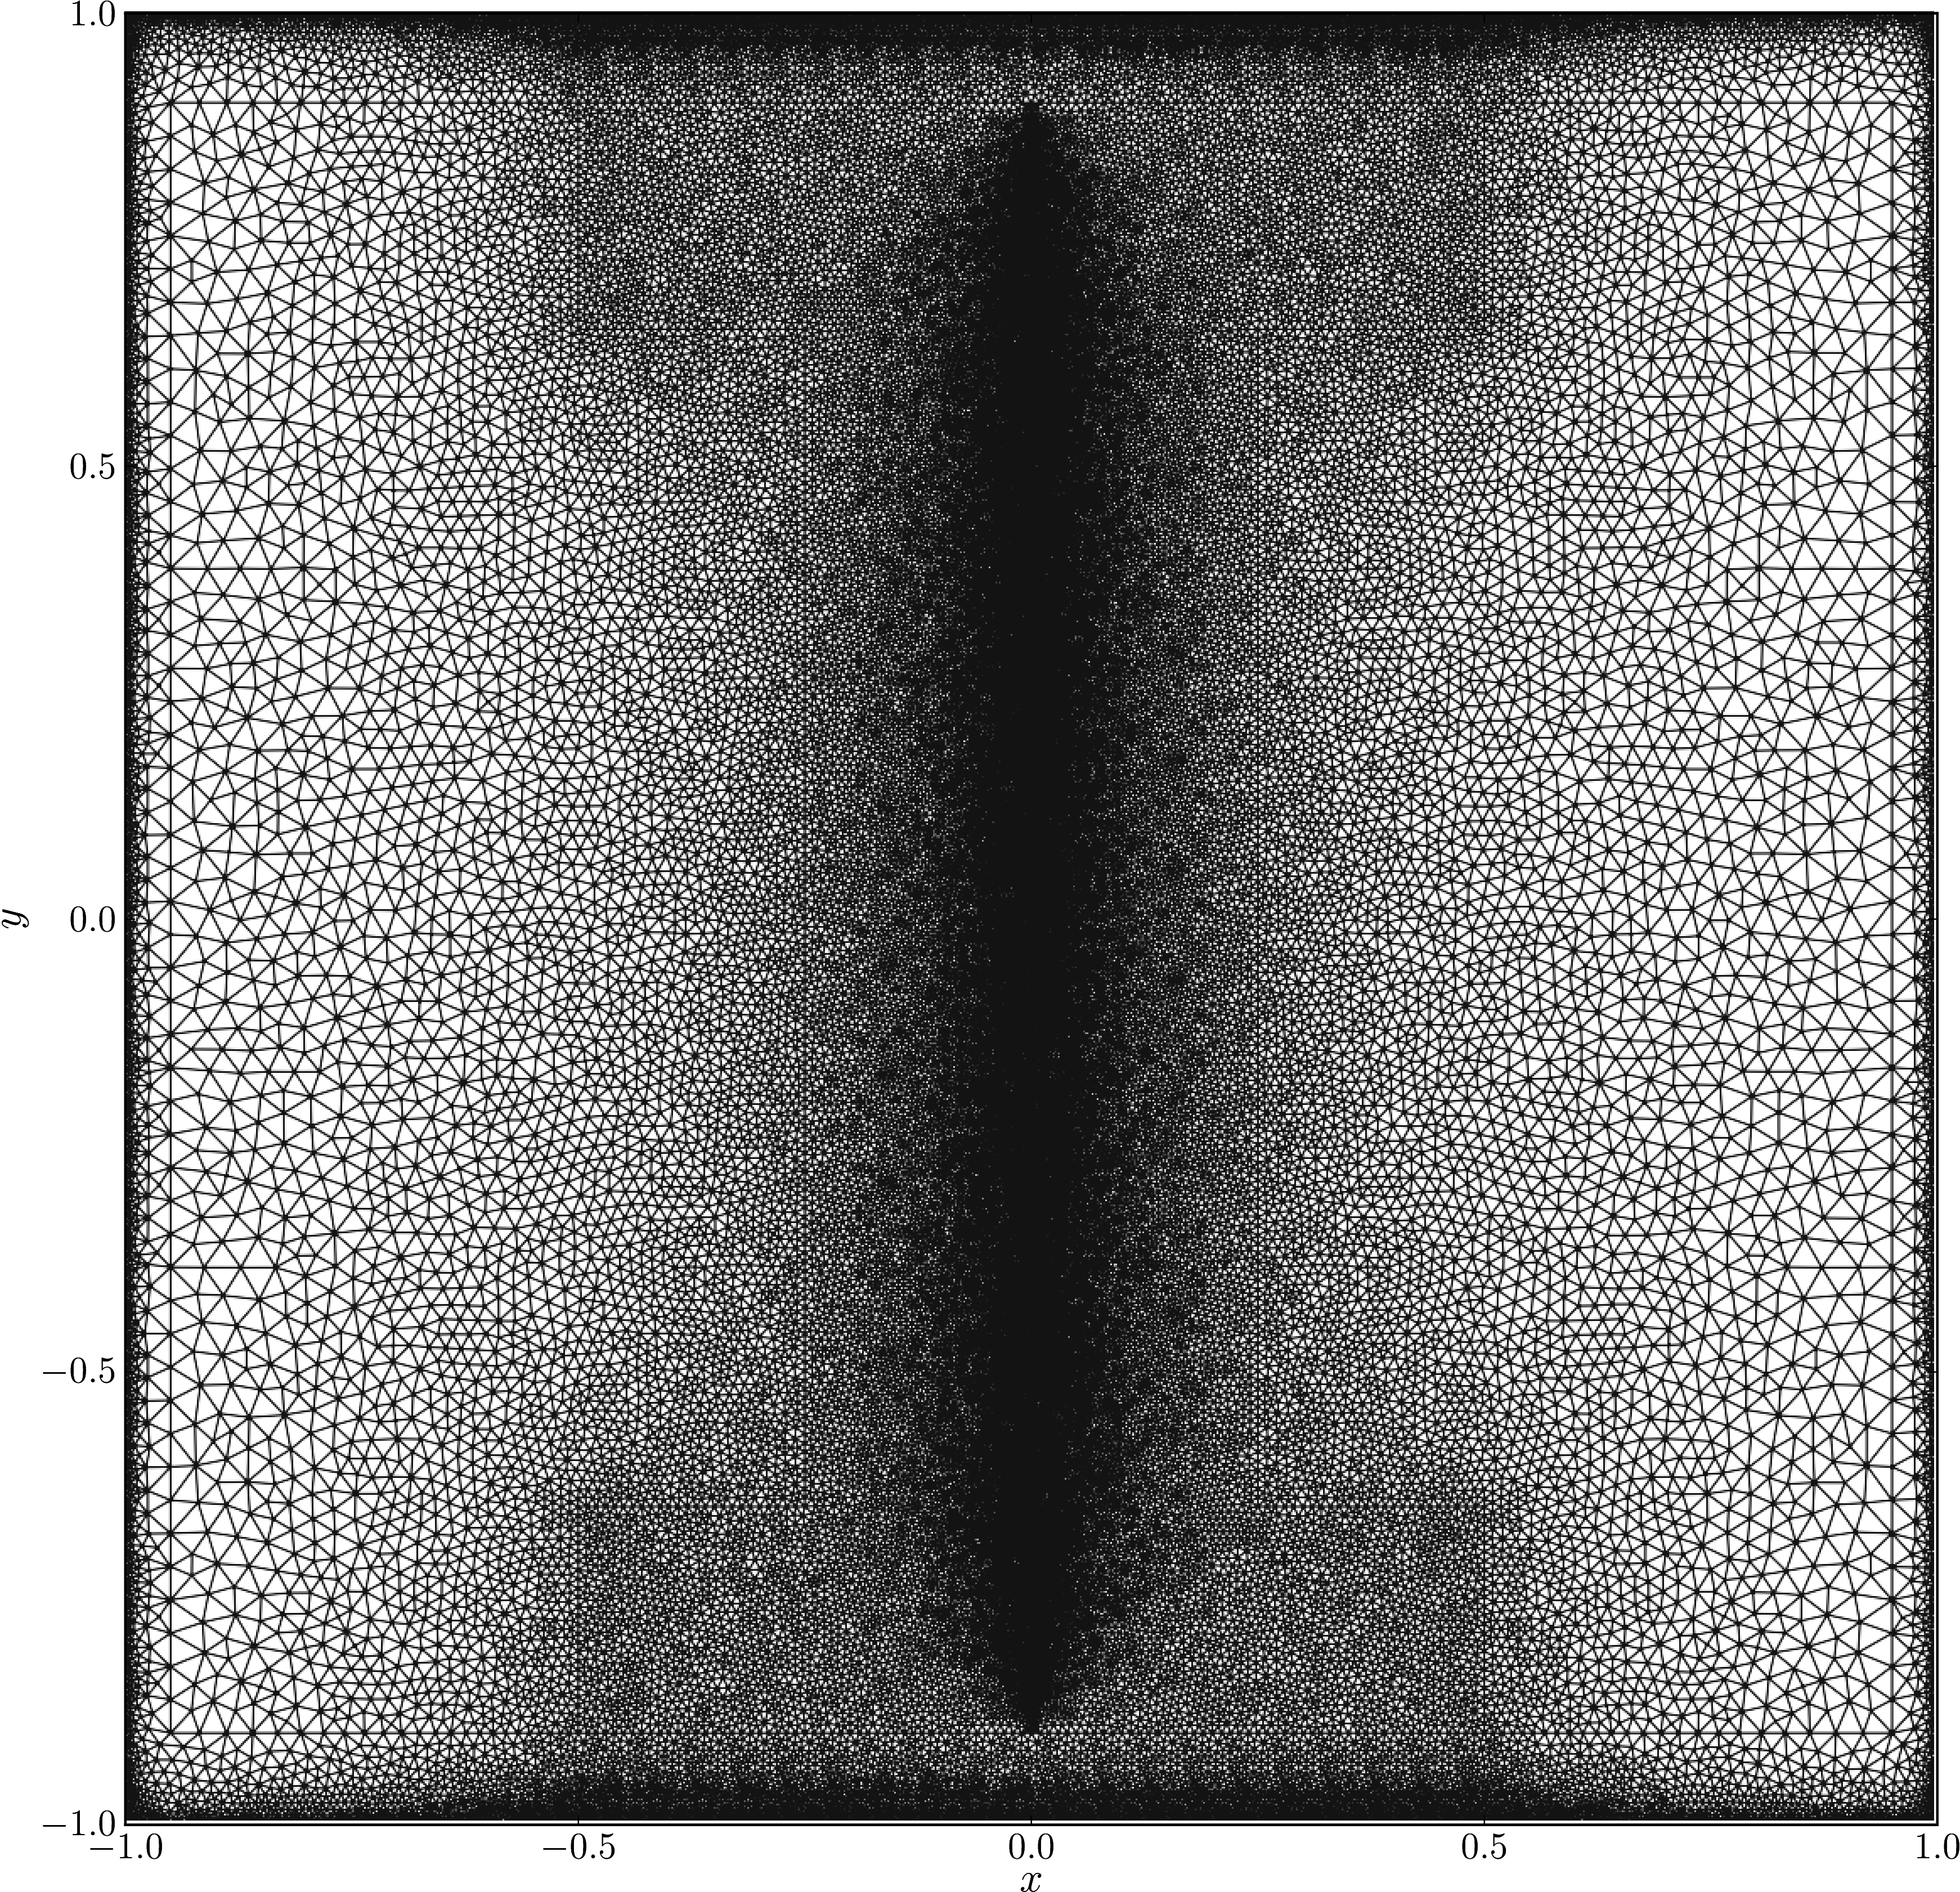
\includegraphics[width=\textwidth]{figures/eulerian/clercxBruneauDomainMesh-crop.png}
             \caption{Domain mesh}
             \label{fig:clercxBruneauDomainMesh}
     \end{subfigure}
     \caption{Domain of the Clercx-Bruneau dipole collision problem. The figure depicts \textbf{(a)} the definition of the domain with the fluid domain ({\color{plotGray}{\textbf{gray}}}) and the no-slip boundary ({\color{plotBlue}{\textbf{blue}}}); and \textbf{(b)} the unstructured mesh of the domain with $N_{\mathrm{vert}} = 48k$.}
     \label{fig:clercxBruneauDomain}
	\end{figure}

For the present study, we have decided to use the simpler case of $Re=625$, where $Re$ is the integral-scale Reynolds number defined as,
	\begin{equation}
	Re = \frac{UW}{\nu},
	\end{equation}
where $U$ is the characteristic velocity of the flow, $W$ is half width of domain, and $\nu$ is the kinematic viscosity and are chosen according to Clercx and Bruneau \cite{Clercx2006a}. A low Reynolds number of $Re=625$ is required as the Eulerian method currently only solves an incompressible laminar flow. However in future, an implementation of a turbulence method can enable a high Reynolds number investigation.

The domain $\Omega$ of the problem is square, $\Omega_E = [-1,1]\times[-1,1]$, as shown in Figure \ref{fig:clercxBruneauDomainDefinition}. The problem is defined in a closed box, where the Eulerian domain is enclosed in a no-slip boundary $\partial{\Omega} = \Sigma_w$ where dipole collides and interacts.

The initial condition of the Clercx-Bruneau dipole is a smooth dipole velocity distribution with a positive monopole at $(x_1,y_1)=(0.1,0)$ and the negative monopole at $(x_2,y_2)=(-0.1,0)$, with each having a core radius $R = 0.1$. The velocity distribution for the combined monopole at $t=0$ is given as,
	\begin{subequations}
	\begin{align}
	u(\mathbf{x},0) & = -\frac{1}{2}\omega_e(y-y_1)\exp\left\{-\left(\frac{r_1}{R}\right)^2\right\} + \frac{1}{2}\omega_e(y-y_2)\exp\left\{-\left(\frac{r_2}{R}\right)^2\right\}, \\
	v(\mathbf{x},0) & = +\frac{1}{2}\omega_e(x-x_1)\exp\left\{-\left(\frac{r_1}{R}\right)^2\right\} - \frac{1}{2}\omega_e(x-x_2)\exp\left\{-\left(\frac{r_2}{R}\right)^2\right\},
	\end{align}
	\label{eq:clercxBruneauVel0}
	\end{subequations}
where $u$ and $v$ are the velocities in the $x$ and $y$ direction, respectively. The characteristic vorticity magnitude $\omega_e = 299.528385375226$ is obtained from Renac et. al \cite{Renac2013}. The radii $r_1$ and $r_2$ are the radial distances to the point $\mathbf{x}$ from the center of positive and the negative monopoles respectively. The corresponding vorticity distribution for the velocity distribution is given as,
	\begin{equation}
	\begin{split}
	\omega(\mathbf{x},0) = \quad &\omega_e\left[1-\left(\frac{r_1}{R}\right)^2\right]\exp\left\{-\left(\frac{r_1}{R}\right)^2\right\} \\
	-\ &\omega_e\left[1-\left(\frac{r_2}{R}\right)^2\right]\exp\left\{-\left(\frac{r_1}{R}\right)^2\right\}.
	\end{split}
	\label{eq:clercxBruneauOmega0}
	\end{equation}

The Eulerian domain was discretized using an unstructured meshing method in GMSH (section \ref{subsec:mgugmsh}), as shown in Figure \ref{fig:clercxBruneauDomainDefinition}. The velocity distribution, equation \ref{eq:clercxBruneauVel0}, shows that the maximum velocity in the fluid will be along the $y$-axis (i.e $x=0$). Therefore, to satisfy the $CFL$ condition, we need the minimum cell size at the location of the maximum velocity. The resolution of the mesh in the region where the dipole and the wall interacts (i.e $-0.5\le{x}\le0.5$ and $0.5\le{\left|y\right|}\le1$) was also increased. Furthermore, in the region where there is no vorticity, we do not need high resolution (i.e $0.5\le{\left|x\right|}\le1$ and $-0.5\le{y}\le0.5$). 

After initializing the velocity field in the discretized domain, the problem was evolved from $t=0$ to $t=2$. The time integration parameters are tabulated in Table \ref{tab:clercxBruneauParameters}.

	\ctable[
		caption = {Summary of the parameters for the Clercx-Bruneau dipole collision with a no-slip wall \cite{Clercx2006a}.},
		label   = {tab:clercxBruneauParameters},
		pos = !t,]{lcll}{\tnote[a]{Obtained from Clercx and Bruneau \cite{Clercx2006a}}
						 \tnote[b]{Obtained from Renac et al. \cite{Renac2013}}}{\FL
		Parameters					& Value 				& Description \ML
		$\Omega$               		& $\left[-1,1\right]\times[-1,1]$ & Eulerian domain bounds \\
		$Re$  			       		& $625$ 				& Reynolds number \\ 
		$U$			         		& $1$\tmark[a]			& Characteristic velocity\\		
		$W$			         		& $1$\tmark[a]			& Half width of the domain\\		
		$\nu$						& $\num{1.6e-3}$ 		& Kinematic viscosity\\
		$ (x,y)_{1,2}$				& $(\pm0.1,0)$			& Initial location of the monopoles\\
		$ \omega_e$		            & $299.5283853752226$\tmark[b]  	&  Characteristic vorticity of the monopole\\
		$ t$ 		    	& 0 to 2				& Simulation time span\\
		$ \mathrm{CFL}$				& $0.95$ 				& CFL number\\	        	        
		$ \lVert\mathbf{u}\rVert_{\mathrm{max}}$	& $12$	& Maximum fluid velocity\\
		$ \Delta t$ 		    	& $\num{1.25e-5}$		& Time step size\\
		$ N_{cells}$ 		& 96142 			& Number of FE mesh cells\\
		$ h_{grid}$			&\num{3.6e-3} to \num{5.1e-2}	        & FE mesh cell size\\	        
		$ N_{t}$ 		& $160,000$	 	& Number of time integration steps\LL}

%	\ctable[
%		caption = {Summary of the parameters for the Clercx-Bruneau normal collision of a dipole with a no-slip wall \cite{Clercx2006a}.},
%		label   = {tab:clercxBruneauParameters},
%		pos = !t,]{lcll}{\tnote[a]{Obtained from Clercx and Bruneau \cite{Clercx2006a}}
%						 \tnote[b]{Obtained from Renac et al. \cite{Renac2013}}}{\FL
%		Parameters					& Value 				& Unit		& Description \ML
%		$\Omega$               		& $\left[-1,1\right]\times[-1,1]$ &\si{m}		& Eulerian domain bounds \\
%		$Re$  			       		& $625$ 				&-			& Reynolds number \\ 
%		$U$			         		& $1$\tmark[a]			&\si{m.s^{-1}}& Characteristic velocity\\		
%		$W$			         		& $1$\tmark[a]			&\si{m}		& Half width of the domain\\		
%		$\nu$						& $\num{1.6e-3}$ 		&\si{kg.s^{-1}.m^{-1}}& Kinematic viscosity\\
%		$ (x,y)_{1,2}$				& $(\pm0.1,0)$			& \si{m}    & Initial location of the dipole\\
%		$ \omega_e$		            & $299.5283853752226$\tmark[b] & -   	&  Characteristic vorticity of the monopole\\
%		$ t$ 		    	& 0 to 2				& - 	& Simulation time\\
%		$ \mathrm{CFL}$				& $0.95$ 				& -			& CFL number\\	        	        
%		$ \lVert\mathbf{u}\rVert_{\mathrm{max}}$	& $12$	& \si{m.s^{-1}}	& Maximum fluid velocity\\
%		$ \Delta t$ 		    	& $\num{1.25e-5}$		& \si{s} 	& Time step size\\
%		$ N_{\mathrm{vert}}$ 		& $\sim48k$ 			& -			& Number of mesh vertices\\
%		$ h_{\mathrm{min}}$			& $\sim\num{3.6e-3}$ &\si{m}		& Minimum mesh cell size\\	        
%		$ N_{\mathrm{tsteps}}$ 		& $160,000$				& -	     	& Number of time integration steps\\
%		$\mathrm{ID}_{\mathrm{fluid}}$ & $1$ 				& - 		& Fluid domain I.D\\
%		$\mathrm{ID}_{\mathrm{wall}}$ & $2$ 				& - 		& No-slip boundary I.D\LL}

%The initial condition of the Clercx-Bruneau dipole is a smooth dipole vorticity distribution with a positive monopole at $(x_1,y_1)=(0.1,0)$ and the negative monopole at $(x_2,y_2)=(-0.1,0)$, with each having a core radius $R = 0.1$. The vorticity distribution of the combined monopole is given as,
%	\begin{equation}
%	\begin{split}
%	\omega(\mathbf{x},0) = \quad &\omega_e\left[1-\left(\frac{r_1}{R}\right)^2\right]\exp\left\{-\left(\frac{r_1}{R}\right)^2\right\} \\
%	-\ &\omega_e\left[1-\left(\frac{r_2}{R}\right)^2\right]\exp\left\{-\left(\frac{r_1}{R}\right)^2\right\} ,
%	\end{split}
%	\label{eq:clercxBruneauOmega0}
%	\end{equation}
%where $\omega_e = 299.528385375226$, obtained from Renac et. al \cite{Renac2013}. The radii $r_1$ and $r_2$ are the radial distances to the point $\mathbf{x}$ from the center of positive and the negative monopoles respectively. Figure \ref{fig:dipole_contourLine_portrait}a shows the vorticity contours of this initial vorticity distribution. The initial vorticity distribution decays at an exponential rate to zero at the no-slip boundary. This means the no-slip boundary condition is still guaranteed for the initial distribution. To initialize the problem in the Eulerian domain with $\mathbf{u}-p$, we used the velocity distribution, 
%	\begin{subequations}
%	\begin{align}
%	u(\mathbf{x},t) & = -\frac{1}{2}\lvert\hat{\omega}_1\rvert(y-y_1)\exp\left\{-\left(\frac{r_1}{R}\right)^2\right\} + \frac{1}{2}\lvert\hat{\omega}_2\rvert(y-y_2)\exp\left\{-\left(\frac{r_2}{R}\right)^2\right\}, \\
%	v(\mathbf{x},t) & = +\frac{1}{2}\lvert\hat{\omega}_1\rvert(x-x_1)\exp\left\{-\left(\frac{r_1}{R}\right)^2\right\} - \frac{1}{2}\lvert\hat{\omega}_2\rvert(x-x_2)\exp\left\{-\left(\frac{r_2}{R}\right)^2\right\},
%	\end{align}
%	\label{eq:clercxBruneauVel0}
%	\end{subequations}
%where $u$ and $v$ are the velocity in the $x$ and $y$ direction, respectively. The fluid domain of the Eulerian domain, show in figure \ref{fig:clercxBruneauDomainDefinition} was discretized using an controlled unstructured meshing method. From the velocity distribution, equation \ref{eq:clercxBruneauVel0}, we see that the maximum velocity in the fluid will be along the $y$-axis (i.e $x=0$). Therefore, to satisfy the $CFL$ condition, we need the minimum cell size at the location of the maximum velocity. Furthermore, to ensure the vorticity generation at the no-slip boundary is defined accurately, we increased resolution of the mesh at the boundary. The third region where we increased the resolution is where the dipole and the wall interacts (i.e $-0.5\le{x}\le0.5$ and $0.5\le{\left|y\right|}\le1$). In the region where there is no vorticity, we do not need high resolution (i.e $0.5\le{\left|x\right|}\le1$ and $-0.5\le{y}\le0.5$). With these parameterization, we obtained an unstructured grid with $N_{\mathrm{vert}}=48k$ vertices.

\subsubsection*{Results and Discussion}

Figure \ref{fig:dipole_contourLine_portrait} shows the evolution of the vorticity field at various instances, $t = [0, 0.25, 0.5,$ $0.75, 1.25]$. During the initial stages of the simulation, the initialized dipole travels along the $y$-axis towards the bottom no-slip boundary. 

	\begin{figure}[!p]
	\centering
	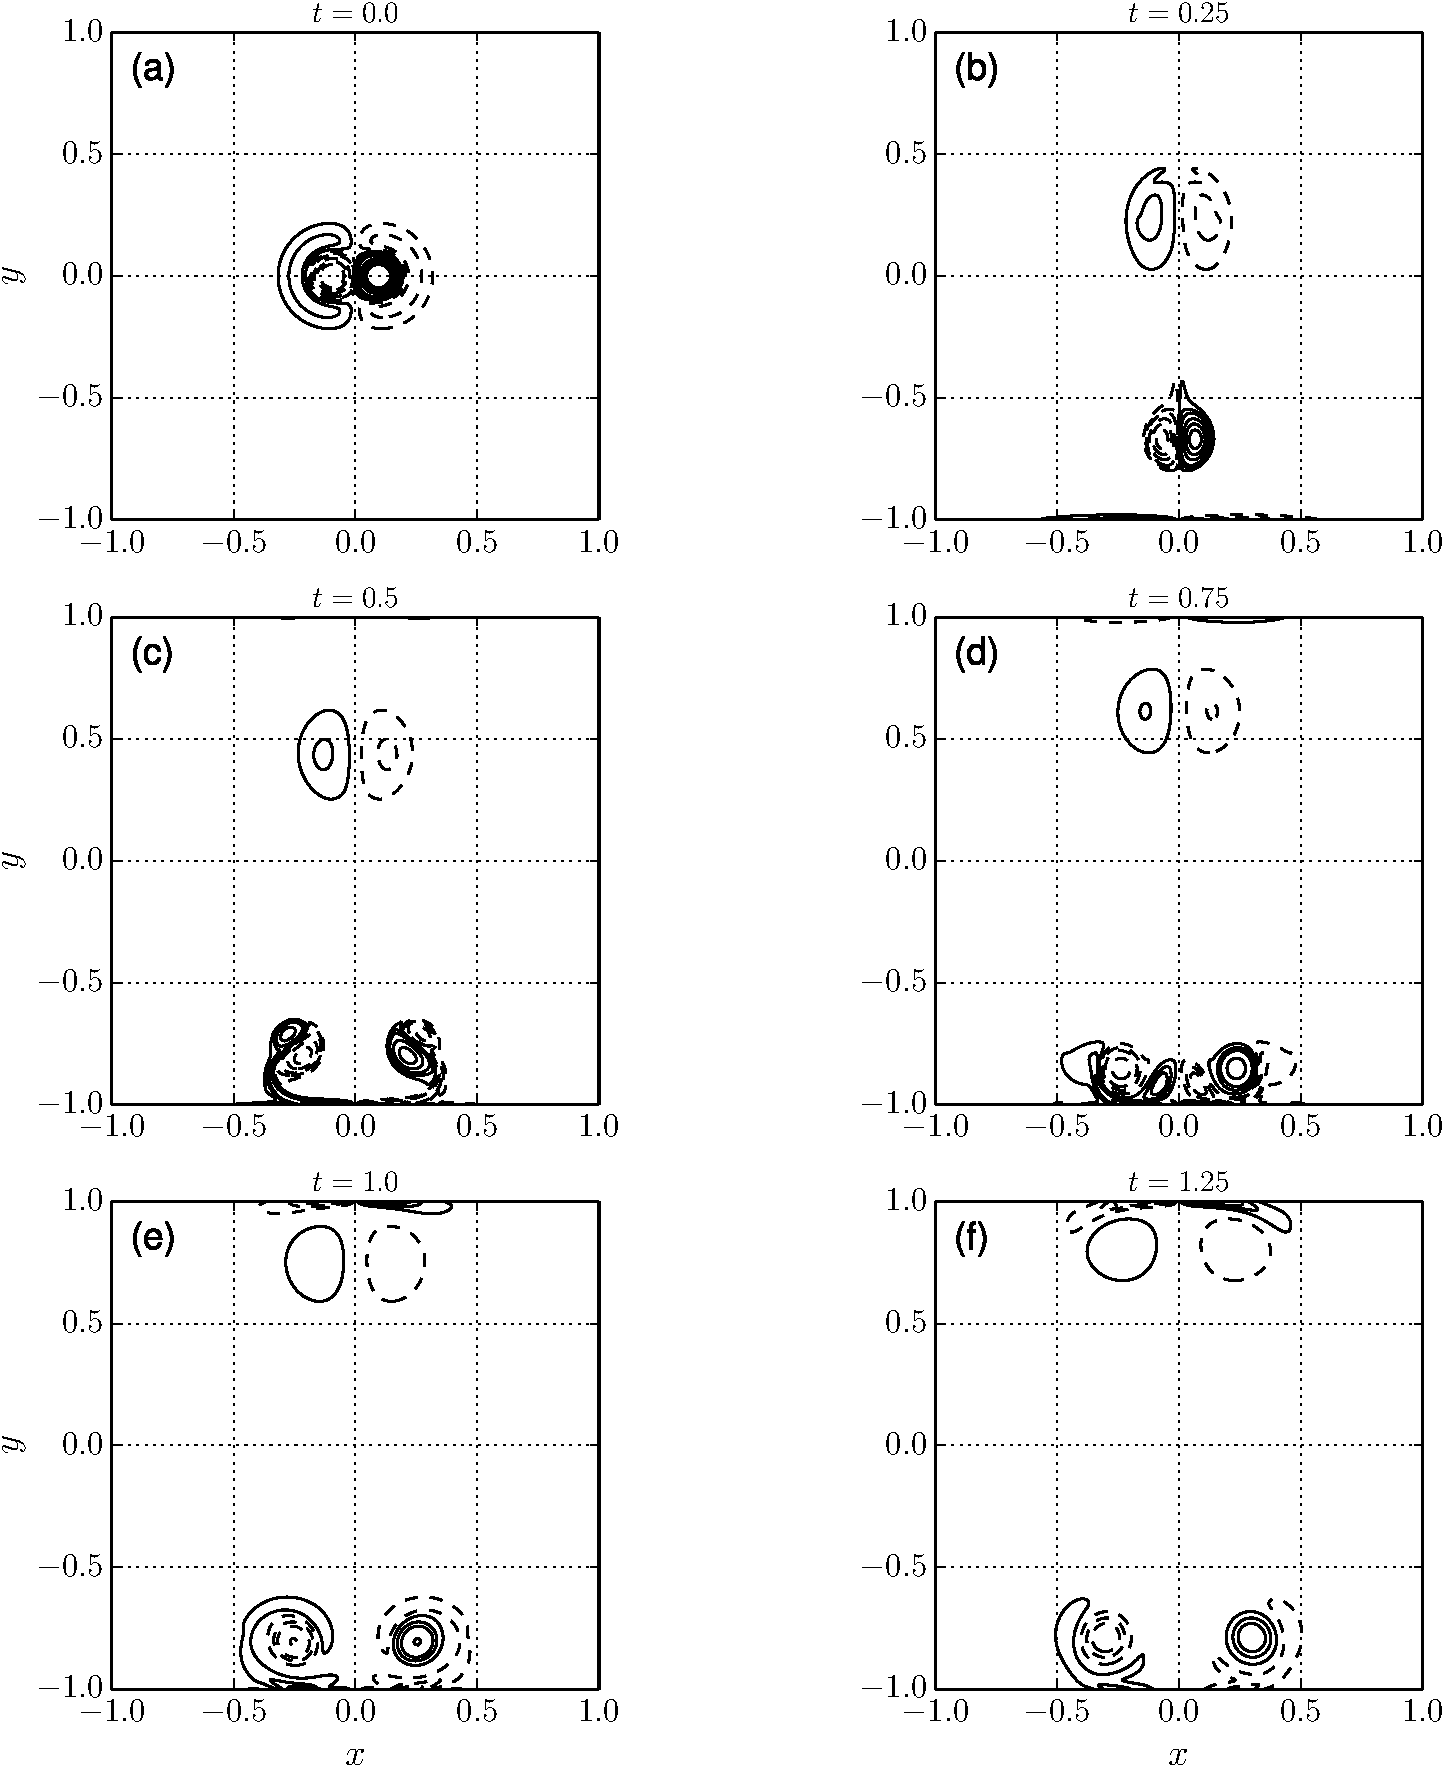
\includegraphics[width=\linewidth]{./figures/eulerian/dipole_contourLine_portrait-crop.pdf}
	\caption{Vorticity contour plots of the Clercx-Bruneau dipole-wall collision at $Re=625$ and $t = [0, 0.25, 0.5, 0.75, 1.0, 1.25]$ with vorticity contour levels at $[-320,-200,-100,$ $-50,-10,10, 50, 100, 200, 320]$. The figure depicts positive contours [---, solid \textbf{black}], and negative contours [- -, dashed \textbf{black}].}
	\label{fig:dipole_contourLine_portrait}
	\end{figure}

The dipole approaches the bottom boundary, where the no-slip boundary generates vorticity to ensure no-through flow, seen in Figure \ref{fig:dipole_contourLine_portrait}{\color{darkblue}{b}}. As the dipole approaches the wall, the vorticity filament at the wall rolls up and combines with the primary dipole forming two secondary dipoles, that is symmetric across the $y$-axis. Figure \ref{fig:dipole_contourLine_portrait}{\color{darkblue}{c}} shows the state of the vorticity field at $t=0.5$ after the secondary dipoles are generated. This secondary dipole initially travels away from the bottom wall and later on approaches the wall again, colliding for a second time and creating a tertiary vortex, Figure \ref{fig:dipole_contourLine_portrait}{\color{darkblue}{d}}. The dipole stops convecting any further and diffuses as time progresses, as shown in Figure \ref{fig:dipole_contourLine_portrait}{\color{darkblue}{e}} and \ref{fig:dipole_contourLine_portrait}{\color{darkblue}{f}}, corresponding to $t = 1$ and $t = 1.25$.

Figure \ref{fig:vorticity_contour_comparison} compares the vorticity contours of the computational domain close to the bottom wall, $0\leqslant x \leqslant 0.6$ and $-1 \leqslant y \leqslant -0.4$, at $t = 1$. The positive vortex (solid black) is surrounded by the negative vortex (dashed black). Comparing the present study, Figure \ref{fig:dipole_contourLine_t1p0} with the study of Clercx and Bruneau \cite{Clercx2006a}, Figure \ref{fig:VorticityContourPlot}, shows that the shows that the shape of the vorticity contours is indistinguishable. This means that the present study matches very well with the pseudo-spectral simulation of the Clercx and Bruneau.

	\begin{figure}[!t]
     \centering
     \begin{subfigure}[t]{0.4\textwidth}
             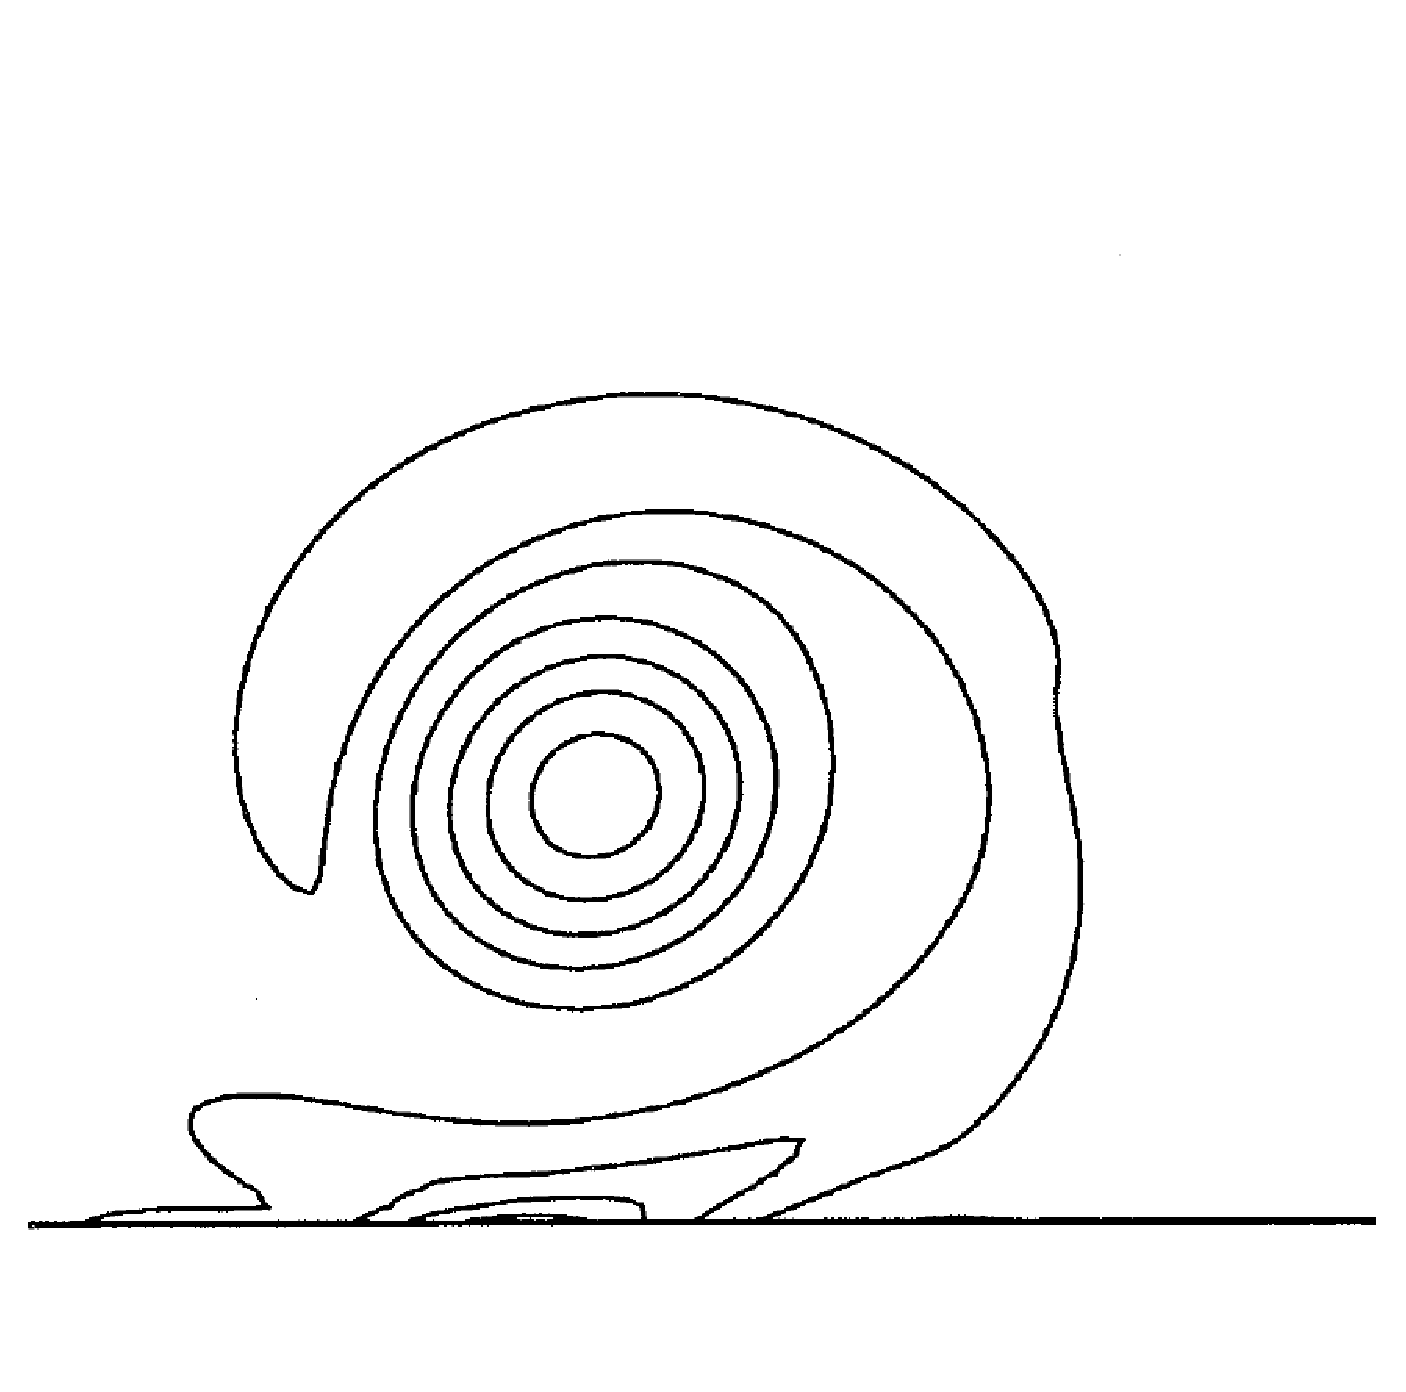
\includegraphics[width=\textwidth]{figures/eulerian/VorticityContourPlot-rotated270.pdf}
             \caption{Literature}
             \label{fig:VorticityContourPlot}
     \end{subfigure}%
     ~ %add desired spacing between images, e. g. ~, \quad, \qquad etc.
       %(or a blank line to force the subfigure onto a new line)
     \begin{subfigure}[t]{0.45\textwidth}
             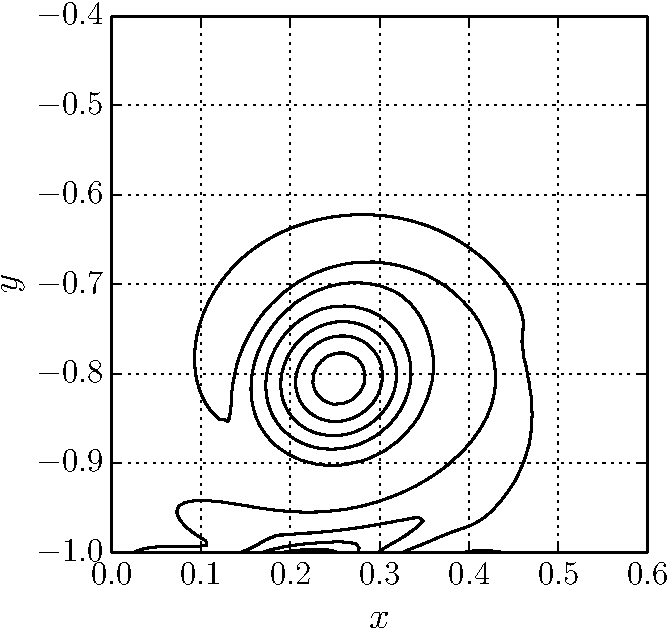
\includegraphics[width=\textwidth]{figures/eulerian/dipole_contourLine_t1p0_corrected-crop.pdf}
             \caption{Present study}
             \label{fig:dipole_contourLine_t1p0}
     \end{subfigure}
     \caption{Comparison of the vorticity contours at $t=1$ with contour levels $[...,-50,$ $-30,-10,10,30,50,...]$. The figure compares the plot obtained by \textbf{(a)} literature of Clercx and Bruneau \cite{Clercx2006a} and \textbf{(b)} the present study.}
     \label{fig:vorticity_contour_comparison}
	\end{figure}
	
	\begin{figure}[!p]
     \centering
     \begin{subfigure}[t]{0.49\textwidth}
             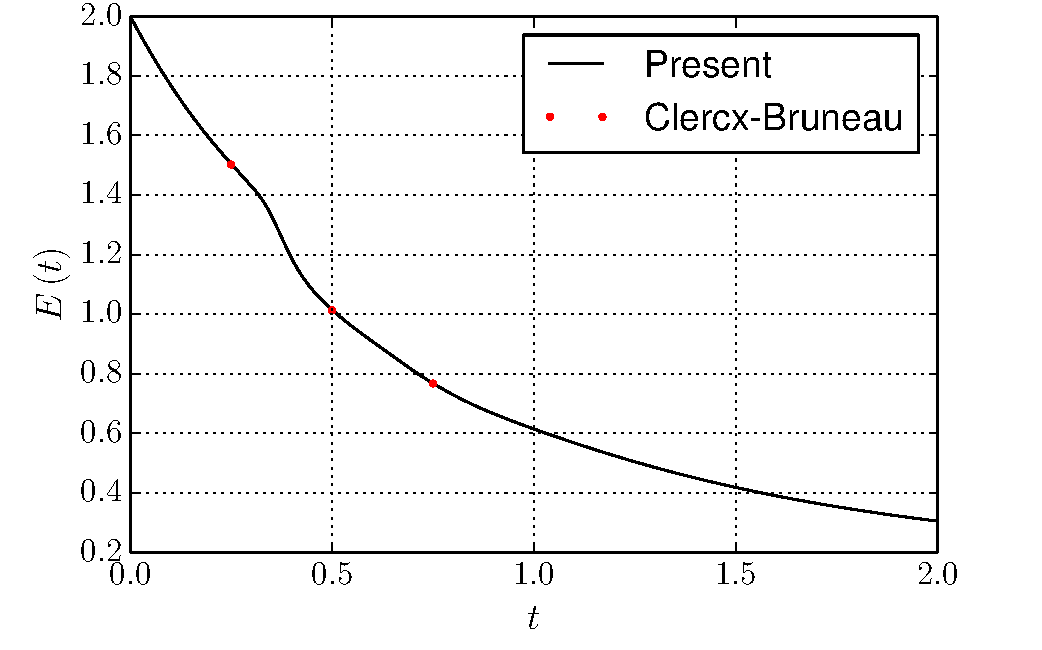
\includegraphics[width=\textwidth]{figures/eulerian/dipole_KineticEnergy_comparison.pdf}
             \caption{Kinetic Energy $E(t)$}
             \label{fig:dipole_KineticEnergy_comparison}
     \end{subfigure}%
     ~ %add desired spacing between images, e. g. ~, \quad, \qquad etc.
       %(or a blank line to force the subfigure onto a new line)
     \begin{subfigure}[t]{0.49\textwidth}
             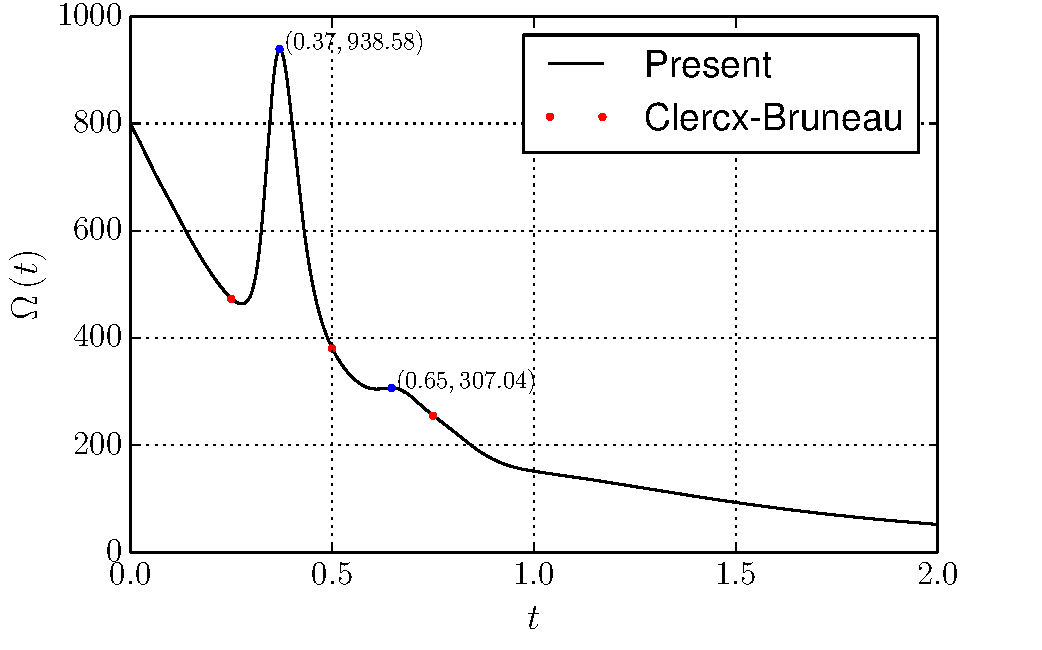
\includegraphics[width=\textwidth]{figures/eulerian/dipole_Enstrophy_comparison.pdf}
             \caption{Enstrophy $\Omega(t)$}
             \label{fig:dipole_Enstrophy_comparison}
     \end{subfigure}
     
     \begin{subfigure}[b]{0.49\textwidth}
             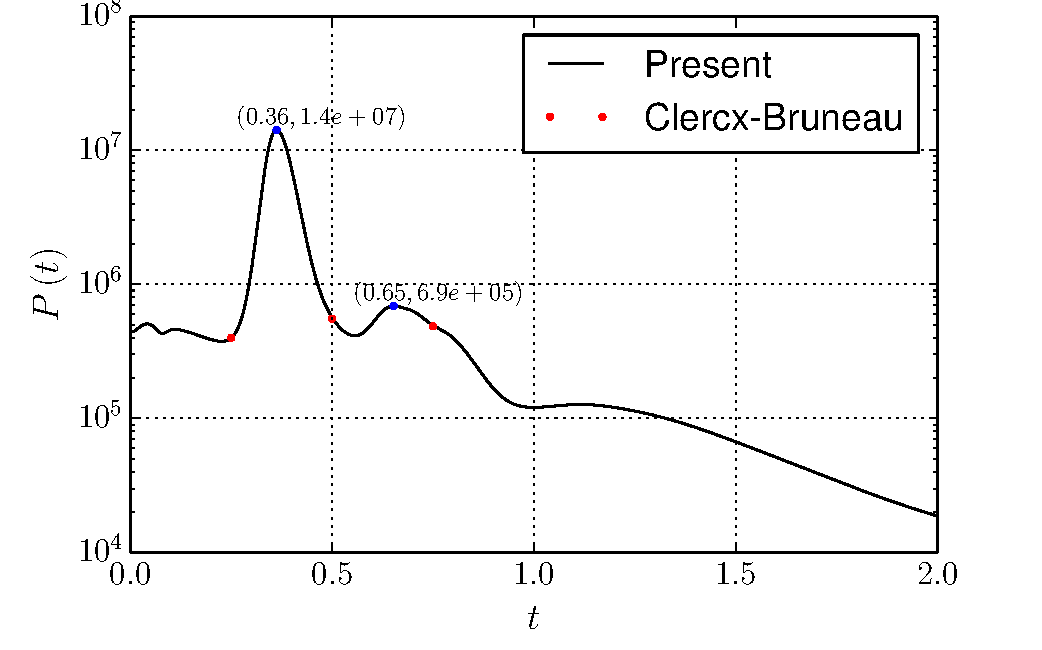
\includegraphics[width=\textwidth]{figures/eulerian/dipole_Palinstrophy_comparison.pdf}
             \caption{Palinstrophy $P(t)$}
             \label{fig:dipole_Palinstrophy_comparison}
     \end{subfigure}
    
     \caption{Comparison of the fluid parameters from $t=0$ to $t=2$ with reference data obtained from Clercx and Bruneau \cite{Clercx2006a} [{\color{plotRed}{$\bullet$}}, {\color{plotRed}{\textbf{red}}} dot]. The figure shows the evolution of \textbf{(a)} the kinetic energy $E(t)$, \textbf{(b)} the enstrophy $\Omega(t)$, and \textbf{(c)} the palinstrophy $P(t)$.}
     \label{fig:dipole_comparison}
	\end{figure}
		
	\begin{figure}[!p]
	\centering
		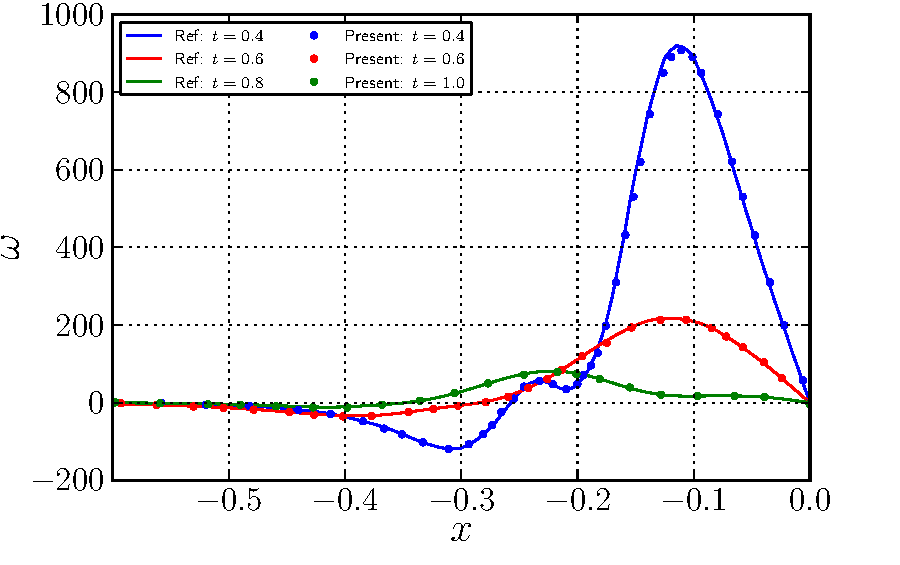
\includegraphics[width=0.6\textwidth]{./figures/eulerian/VorticityAtBoundary2.pdf}
		\caption{The vorticity generated at the bottom-left wall ($y=-1$, $-0.6\leqslant x \leqslant 0$) at $t=0.4$ [{\color{plotBlue}{---}}, solid blue], $t=0.6$ [{\color{plotRed}{---}}, solid red] and $t=1$ [{\color{plotGreen}{---}}, solid green]. The results are compared with Clercx and Bruneau \cite{Clercx2006a} (dotted).}
		\label{fig:VorticityAtBoundary}
	\end{figure}	
	
To determine the variation of the fluid properties as time progresses, Clercx and Bruneau investigated the evolution of the total kinetic energy $E$, the total enstrophy $\Omega$, and the total palinstrophy $P$ of the flow field. The total kinetic energy $E$ of the flow can be determined with,
	\begin{equation}
	E(t) = \frac{1}{2} \int\int \mathbf{u}^2(\mathbf{x},t)\ \mathrm{d}x\mathrm{d}y,
	\end{equation}
and at $t=0$, we have $E(0) = 2$. The total enstrophy of the flow is determined as, 
	\begin{equation}
	\Omega(t) = \frac{1}{2}\int\int\omega^2(\mathbf{x},t)\ \mathrm{d}x\mathrm{d}y.
	\end{equation}	
The change in enstrophy of the flow field can give an insight into the dissipation rate in the fluid. At $t=0$, the total enstrophy of the fluid is $\Omega(0)=800$. The total palinstrophy $P$ of the flow measures the gradient of vorticity and is given by, 
	\begin{equation}
	P(t) = \frac{1}{2}\int\int\left[\nabla\omega(\mathbf{x},t)\right]^2\ \mathrm{d}x\mathrm{d}y,
	\end{equation}
and gives an insight into the generation of vorticity at the no-slip boundary. Figure \ref{fig:dipole_comparison} compares the evolution of these time dependent parameters with the reference data provided by Clercx and Bruneau. Clercx and Bruneau \cite{Clercx2006a} provide the values of the parameters at $t=0.25$, $t=0.5$ and $t=0.75$. 

Figure \ref{fig:dipole_KineticEnergy_comparison} shows the evolution of the kinetic energy. The kinetic energy $E$ reduced from $E(0) = 2$ to $E(2) \approx 0.3$. At $t=0.4$, we have small kink representing the approach of the primary dipole at the wall. When plotting the reference data, we see that the variation in kinetic energy matches perfectly at $t=0.25$, $t=0.5$ and $t=0.75$.

%	\ctable[
%	    caption = {A summary of the values of the first two maxima of the enstrophy $E$ and palinstrophy $P$ occurring at $t_1$ and $t_2$ respectively.},
%	    label   = {tab:euleriandipoleCollisionComparison},
%	    maxwidth = \textwidth,
%	    pos = !t,
%	]{ccrrrr}{\tnote{Data obtained from Clercx \& Bruneau \cite{Clercx2006a}}}{\FL
%	\multirow{2}{*}{Instant} & 	\multirow{2}{*}{Case} & \multicolumn{2}{c}{Enstrophy $\Omega$} & \multicolumn{2}{c}{Palinstrophy $P$}\\
%	\noalign{\smallskip}\cline{3-6}\noalign{\smallskip}
%			& 			& $t$ & $\Omega$ 	& $t$ & $P$\ML
%	\multirow{2}{*}{$1^{\mathrm{st}} peak$} 	& Reference\tmark[a] 	& 0.371 & 933.6 	& 0.361 & $1.39\times10^7$\\
%							& Present 		& 0.370 & 938.6 	& 0.360 & $1.40\times10^7$\\
%	\multirow{2}{*}{$2^{\mathrm{nd}} peak$} 	& Reference\tmark[a] 	& 0.648 & 305.2 	& 0.652 & $6.78\times10^{5}$\\
%							& Present 		& 0.650 & 307.0		& 0.650 & $6.90\times10^{5}$\LL}

%	\ctable[
%	    caption = {A summary of the values of the first two maxima of the enstrophy $E$ and palinstrophy $P$ occurring at $t_1$ and $t_2$ respectively.},
%	    label   = {tab:euleriandipoleCollisionComparison},
%	    maxwidth = \textwidth,
%	    pos = !t,
%	]{ccrr}{\tnote{Data obtained from Clercx \& Bruneau \cite{Clercx2006a}}}{\FL
%	\multirow{2}{*}{Instant} & 	\multirow{2}{*}{Case} & \multicolumn{2}{c}{$t$}\\
%	\noalign{\smallskip}\cline{3-4}\noalign{\smallskip}
%			& 			& Enstrophy $\Omega$ & Palinstrophy $P$ \ML
%	\multirow{2}{*}{$1^{\mathrm{st}}$ peak} 	& Reference\tmark[a] 	& 0.371 & 0.361 \\
%							& Present 		& 0.370 & 0.360 \\ \\ 
%	\multirow{2}{*}{$2^{\mathrm{nd}}$ peak} 	& Reference\tmark[a] 	& 0.648 & 0.652 \\
%							& Present 		& 0.650 & 0.650 \LL}


Figure \ref{fig:dipole_Enstrophy_comparison} shows the evolution of enstrophy $\Omega$ in time. During the initial instants, enstrophy decreases linearly and at $t=0.370$, there is sharp increase in the total enstrophy of the flow $\Omega(0.370) = 938.58$ (shown in blue). This indicates the initial impact of dipole with the no-slip wall. However, in literature \cite{Clercx2006a}, the initial peak occurs at $t=0.371$ with a peak enstrophy of $\Omega(0.371)=938.6$. Comparing these parameters we see that the enstrophy we calculate peaks earlier and with a larger values, meaning that our collision is slight early. However, the error in time of peaking is $0.3\%$ with a $0.6\%$ error in enstrophy, which is a significantly small error. We observe similar behaviour in the second collision, where the peak is our study is $\Omega(0.650)=307.04$ (shown in blue), whereas in literature the peak is $\Omega(0.648) = 305.2$. Again the error is relatively small implying that our Eulerian method resolves the evolution of enstrophy very well.

%After the impact, the enstrophy quickly drops and peaks again at $t=0.65$ reaching $\Omega(0.65) = 307.04$. Table \ref{tab:euleriandipoleCollisionComparison} shows the occurrence of the peak enstrophy for Clercx and Bruneau ??. We see that in the study of Clercx and Bruneau, the first peak occurred at $t=0.371$ and the second peak occured at $t=0.648$. This means a $0.3\%$ and a $0.6\%$ error in time for occurrence of the peak in enstrophy. The 

% implying that our Eulerian method resolves the evolution of enstrophy very well.

%In addition, to the 3 data points, Clercx \& Bruneau determined the peak enstrophy of flow. Table \ref{tab:euleriandipoleCollisionComparison} compares the difference between the present study and literature and we see that there is maximum of $0.3\%$ error in time $t$ and $0.6\%$ error in enstrophy $\Omega$. Therefore, the variation in enstrophy is well represented by our Eulerian method.

Figure \ref{fig:dipole_Palinstrophy_comparison} shows the evolution of palinstrophy $P$ in time. When the dipole collides, vorticity is generated from the wall to ensure no-through boundary condition, which results in a sharp increase in the gradient of the vorticity.  Similar to the evolution of enstrophy, we can observe to peaking at $t=0.360$ and $t=0.650$, with peak palinstrophy of $P(0.360)=1.40\times10^7$ and $P(0.650)=6.90\times10^{5}$, respectively (shown in blue). In literature however, the peak palinstrophy occurs at $P(0.361) =1.39\times10^7$ and 
$P(0.652)=6.78\times10^{5}$. This is an acceptable error and tells us the generation of vorticity in Eulerian method performs according to theory.

%Table \ref{tab:euleriandipoleCollisionComparison} compares the difference with the addition data provided and we see that there is a maximum error of $0.3\%$ in time $t$ and $1.8\%$ in palinstrophy $P$. This is an acceptable error and tells us the generation of vorticity in Eulerian method performs according to theory.
	
Figure \ref{fig:VorticityAtBoundary} compares the vorticity along the boundary of the domain at $y=-1$ for $-0.6 \leqslant x \leqslant 0$. The solid lines represent the present data, and is compared with the dotted data obtained from Clercx and Bruneau \cite{Clercx2006a}. The comparison is done for various time instances $t=0.4$, $t=0.6$ and $t=1.0$ and we can finally validate that the Eulerian method accurately represents vorticity generation from the wall.


%	\begin{figure}[p]
%     \centering
%     \begin{subfigure}[t]{0.49\textwidth}
%             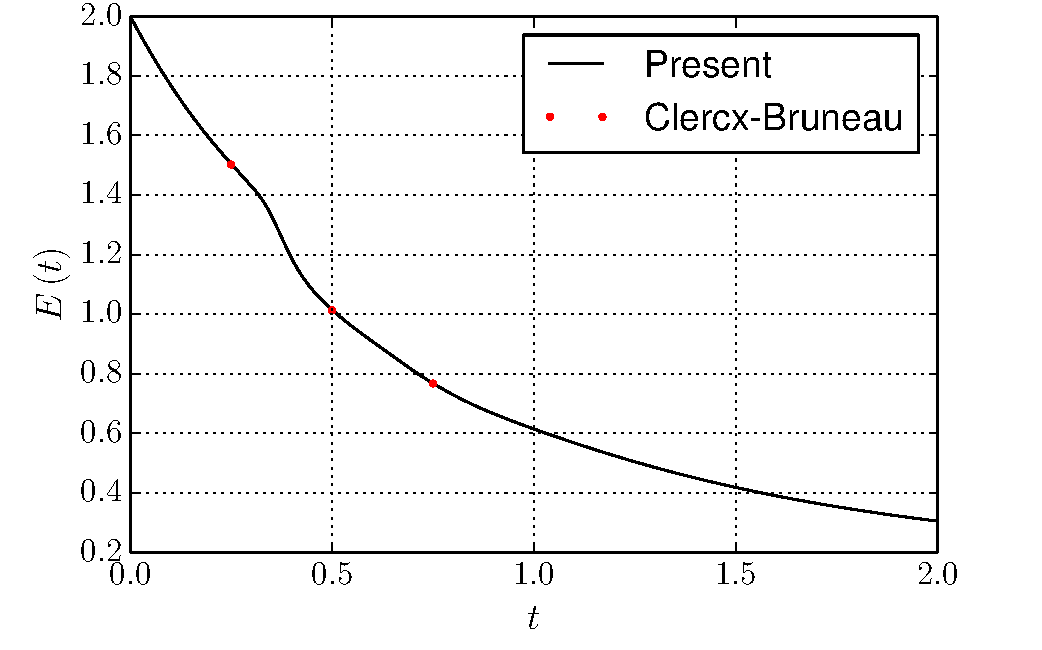
\includegraphics[width=\textwidth]{figures/eulerian/dipole_KineticEnergy_comparison.pdf}
%             \caption{Kinetic Energy $E(t)$}
%             \label{fig:dipole_KineticEnergy_comparison}
%     \end{subfigure}%
%     ~ %add desired spacing between images, e. g. ~, \quad, \qquad etc.
%       %(or a blank line to force the subfigure onto a new line)
%     \begin{subfigure}[t]{0.49\textwidth}
%             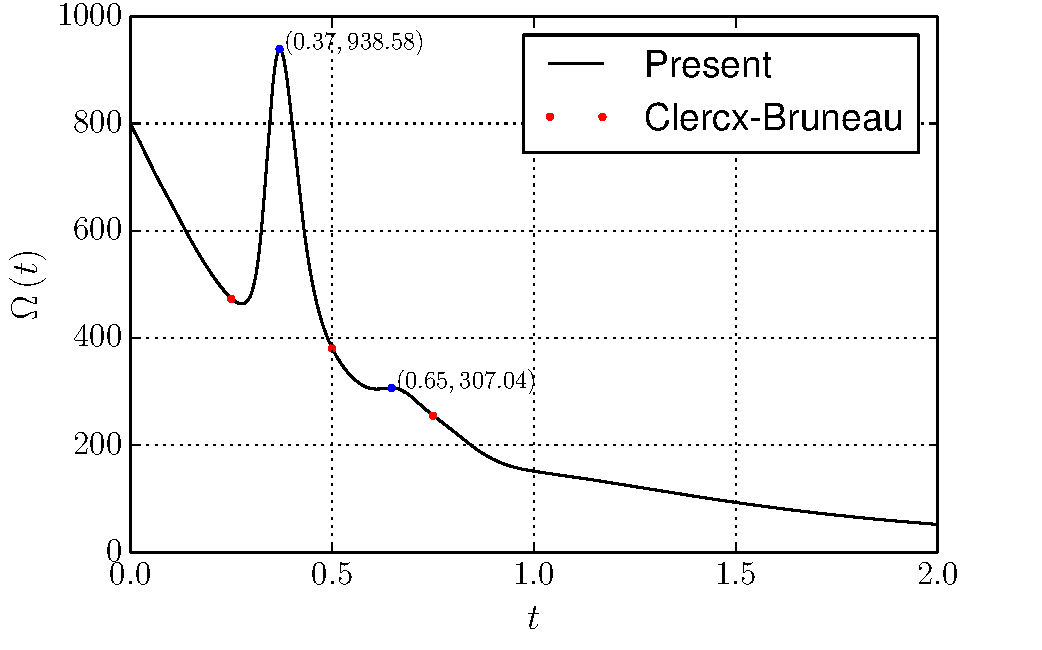
\includegraphics[width=\textwidth]{figures/eulerian/dipole_Enstrophy_comparison.pdf}
%             \caption{Enstrophy $\Omega(t)$}
%             \label{fig:dipole_Enstrophy_comparison}
%     \end{subfigure}
%     
%     \begin{subfigure}[b]{0.49\textwidth}
%             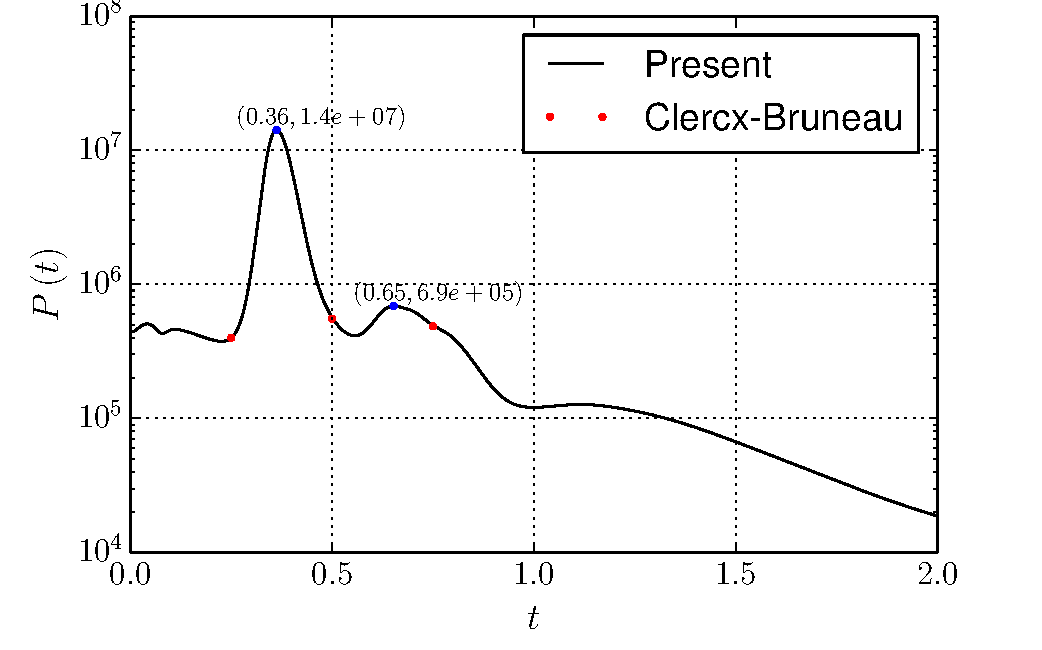
\includegraphics[width=\textwidth]{figures/eulerian/dipole_Palinstrophy_comparison.pdf}
%             \caption{Palinstrophy $P(t)$}
%             \label{fig:dipole_Palinstrophy_comparison}
%     \end{subfigure}
%     ~
%     \begin{subfigure}[b]{0.48\textwidth}
%		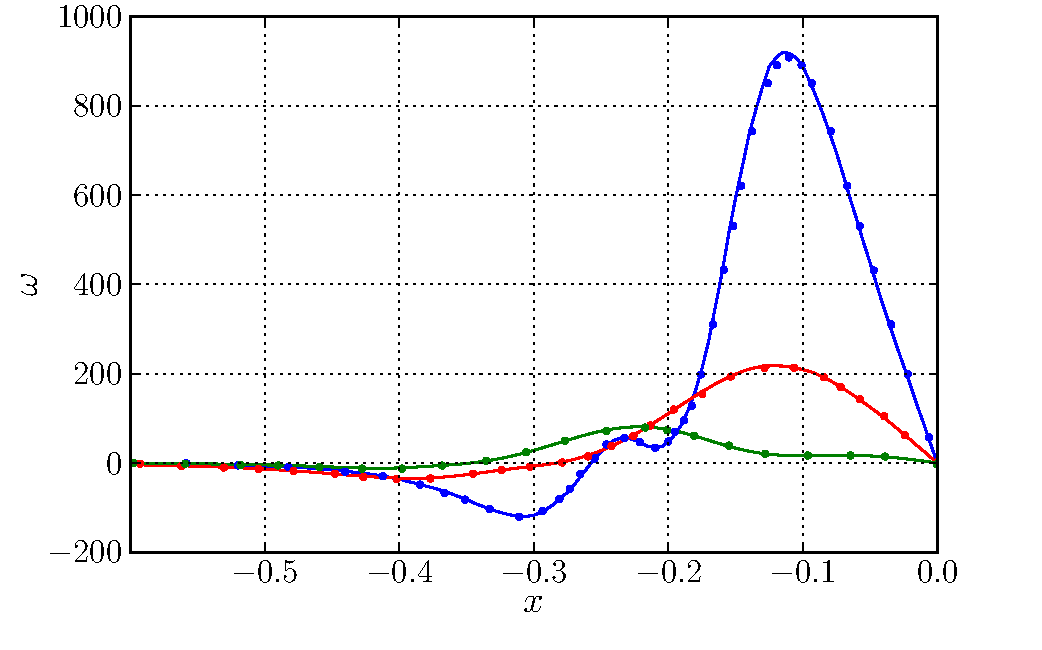
\includegraphics[width=\textwidth]{./figures/eulerian/VorticityAtBoundary.pdf}
%		\caption{Vorticity at the boundary y = -1.}
%		\label{fig:VorticityAtBoundary}
%     \end{subfigure}     
%     
%     \caption{Comparison of the fluid parameters. Figure \textbf{(a)}, \textbf{(b)}, \textbf{(c)} compares the evolution of the fluid properties from $t=0$ to $t=2$. Figure \textbf{(d)} compares the vorticity generated at the bottom-left wall ($y=-1$, $-0.6\leqslant x \leqslant 0$) at $t=0.4$ [{\color{plotBlue}{---}}, solid blue], $t=0.6$ [{\color{plotRed}{---}}, solid red] and $t=1$ [{\color{plotGreen}{---}}, solid green].}
%     \label{fig:dipole_comparison}
%	\end{figure}

\subsection{Impulsively Started Cylinder at $Re=550$}
\label{subsec:eul_isc}
Finally, we an impulsively started cylinder at $Re=550$. This validation test ensured that we are able to determine correct forces acting on the body. 

\subsubsection*{Problem Definition}

	\begin{figure}[!p]
     \centering
     \begin{subfigure}[t]{0.45\textwidth}
             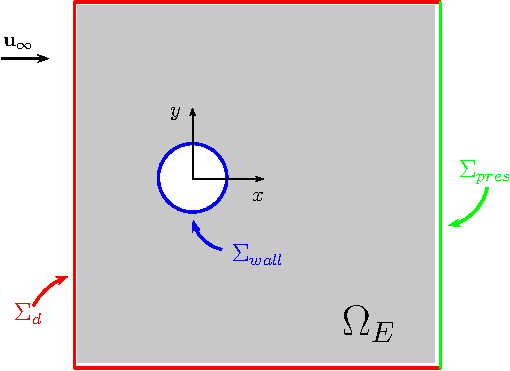
\includegraphics[width=\textwidth]{figures/eulerian/ISCDomainDefinition-crop.pdf}
             \caption{(\textit{Not to scale}) Domain definition}
             \label{fig:ISCDomainDefinition-crop}
     \end{subfigure}%
     ~ %add desired spacing between images, e. g. ~, \quad, \qquad etc.
       %(or a blank line to force the subfigure onto a new line)
     \begin{subfigure}[t]{0.45\textwidth}
             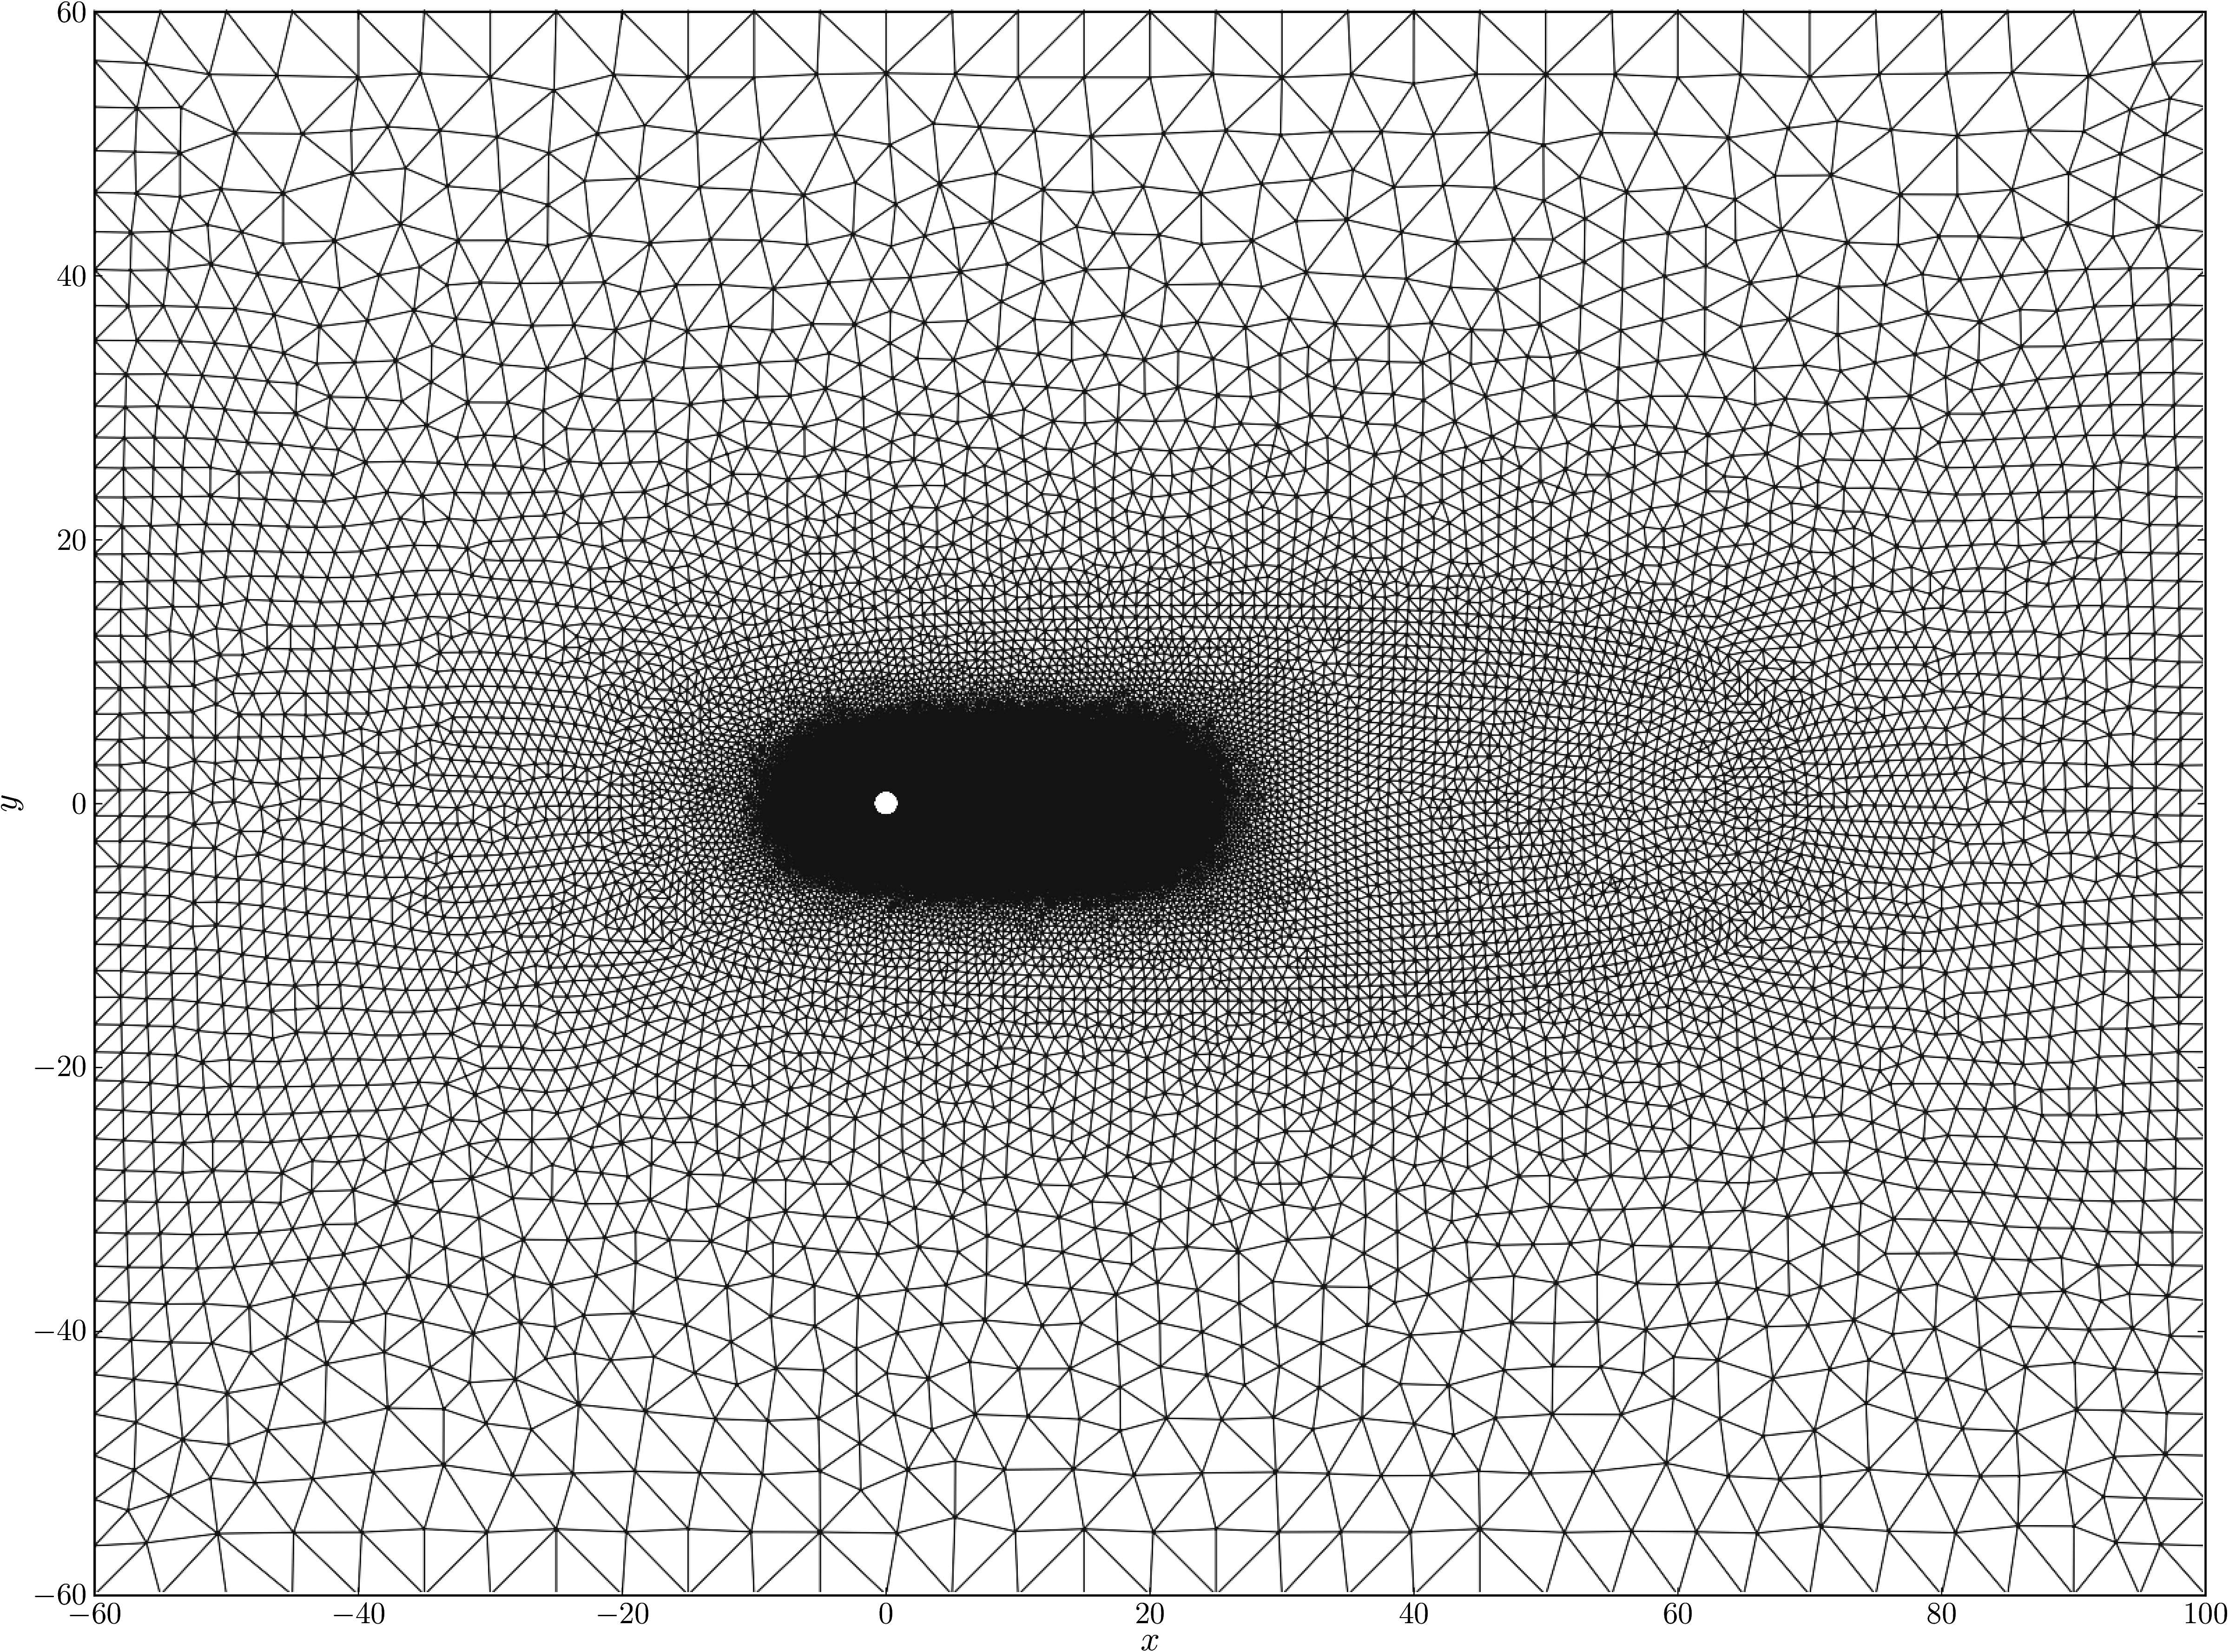
\includegraphics[width=\textwidth]{figures/eulerian/ISC_mesh-crop.png}
             \caption{Full mesh}
             \label{fig:ISC_mesh}
     \end{subfigure}

     \begin{subfigure}[t]{0.3\textwidth}
             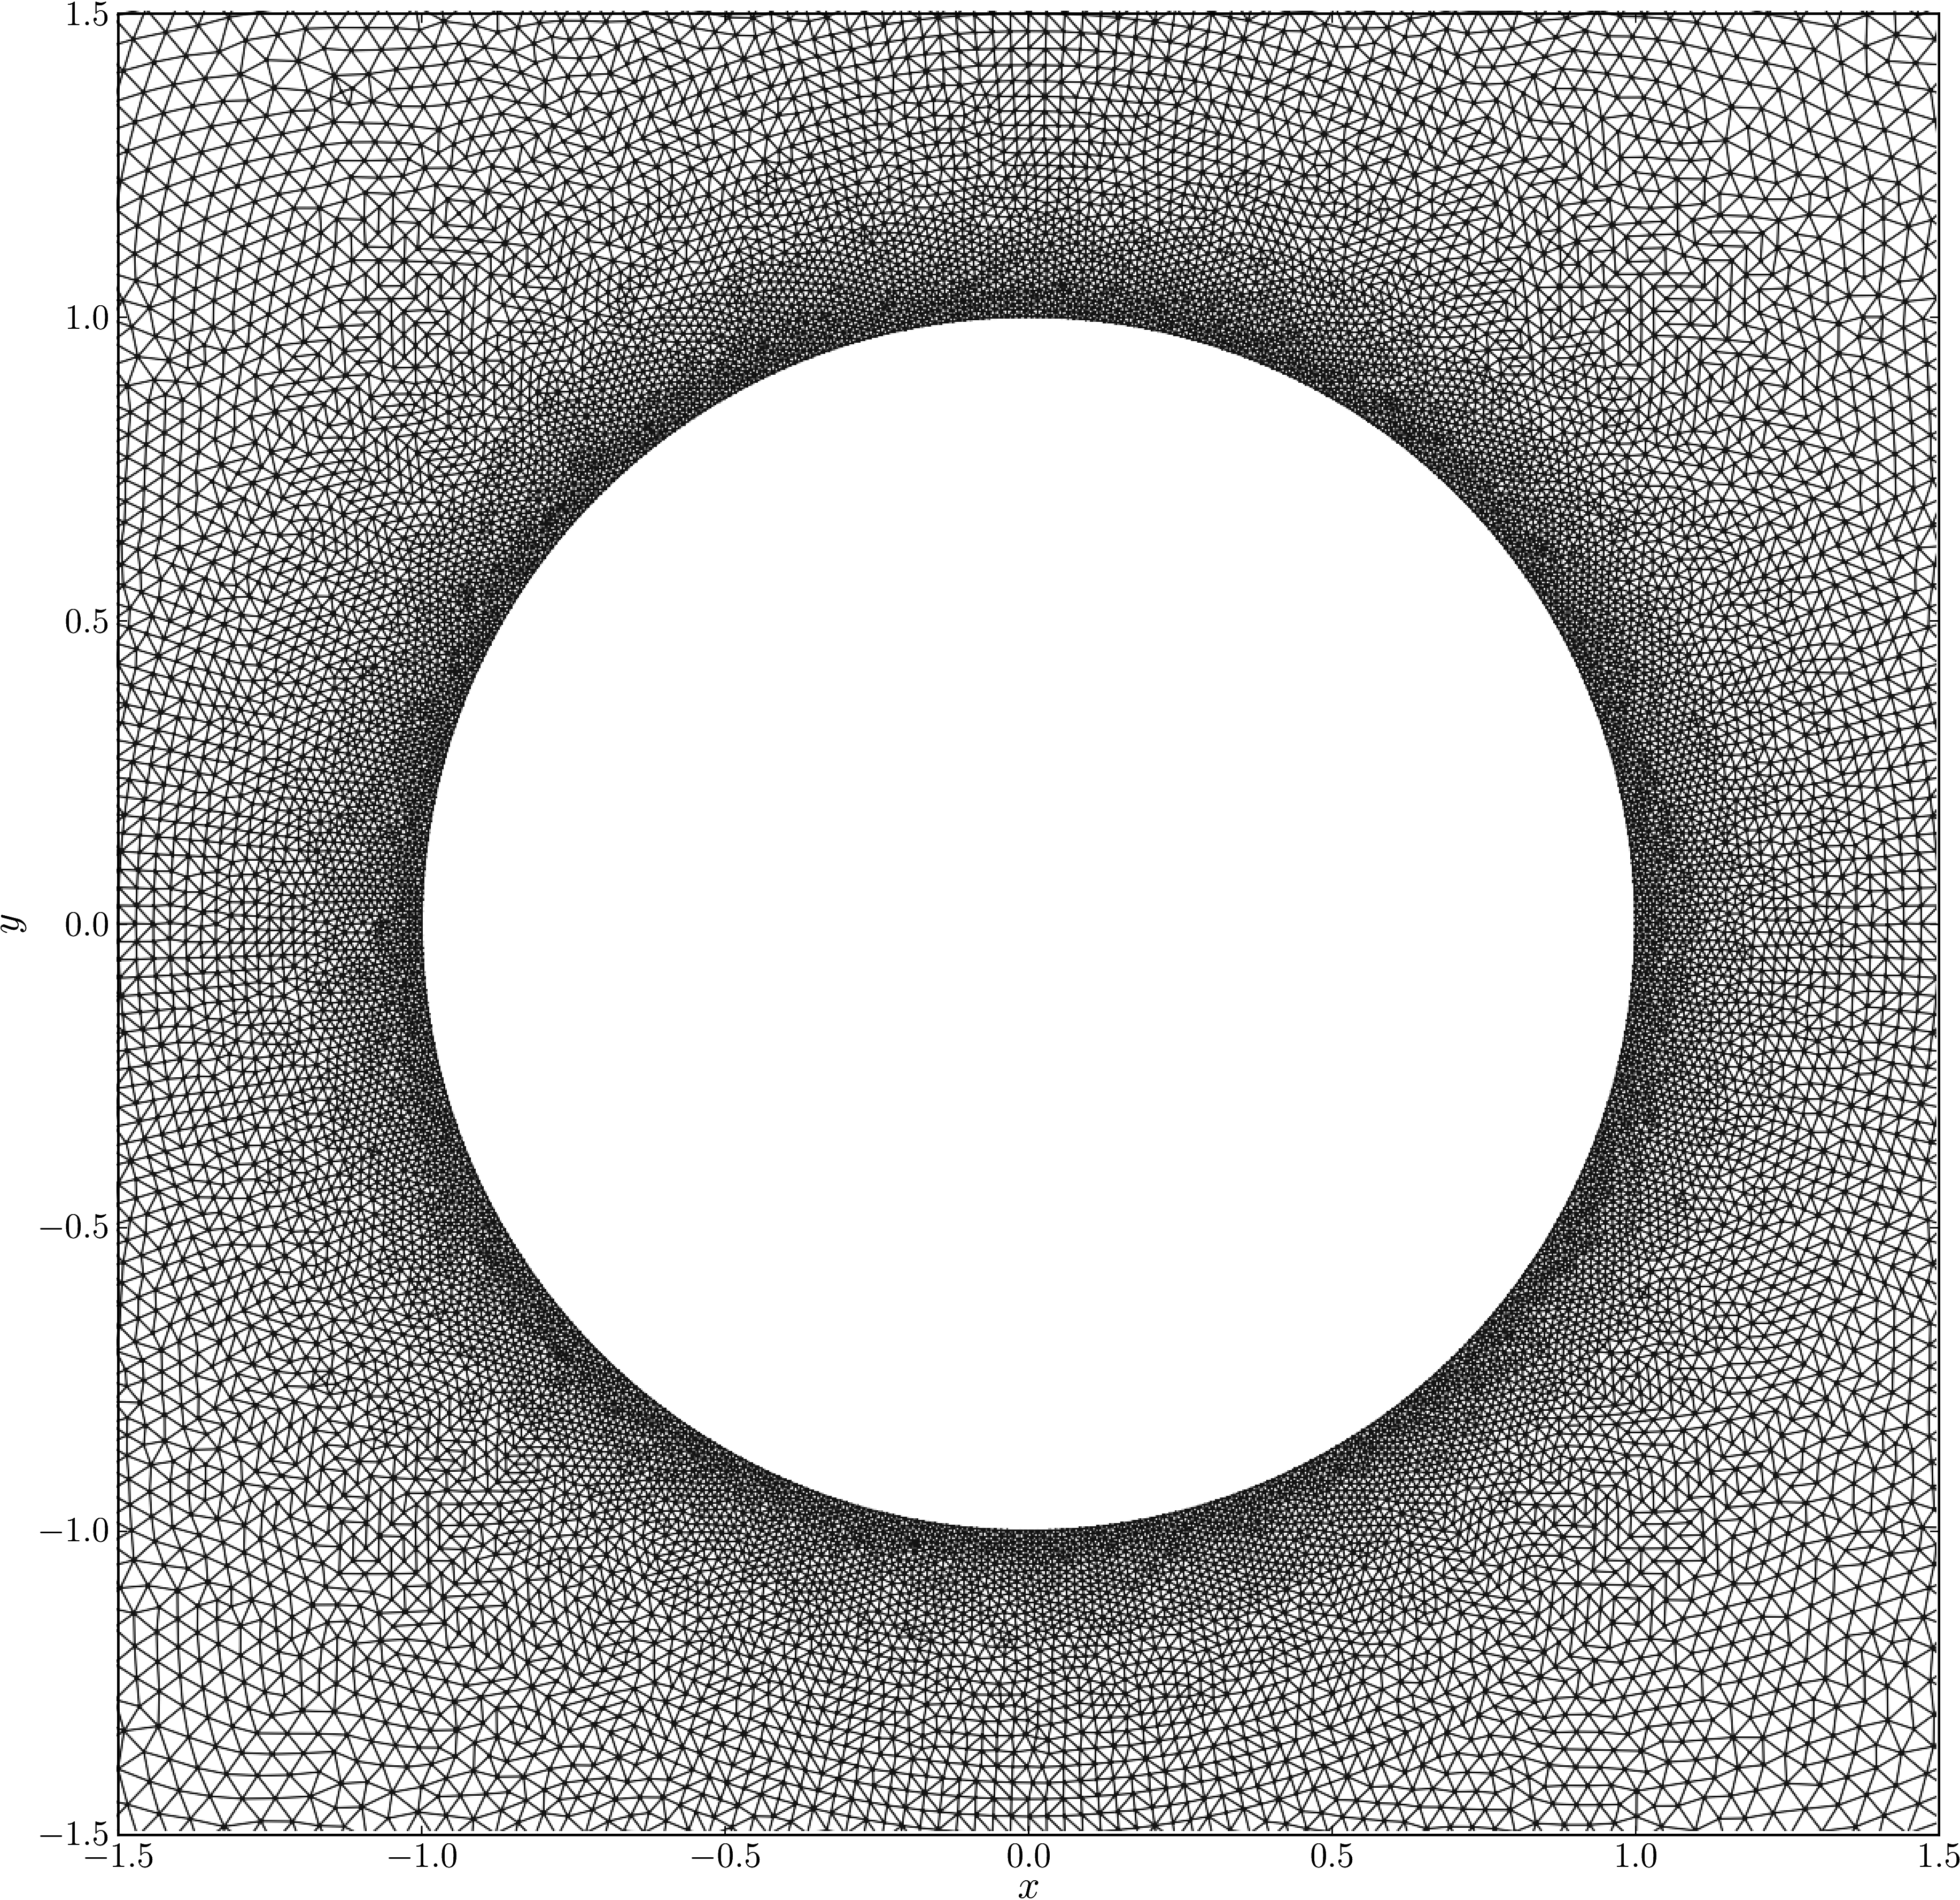
\includegraphics[width=\textwidth]{figures/eulerian/ISC_mesh_surface-crop.png}
             \caption{Mesh near the surface}
             \label{fig:ISC_mesh_surface}
     \end{subfigure}

     \caption{Domain of the ISC problem. The figure depicts \textbf{(a)} the definition, \textbf{(b)} the full domain mesh, and \textbf{(c)} the mesh near the surface.}
     \label{fig:ISCDomain}
	\end{figure}

%	\ctable[
%		caption = {Summary of the parameters for the Impulsively started cylinder test case for $Re=550$.},
%		label   = {tab:ISCParameters},
%		pos = !p,]{lcll}{}{\FL
%		Parameters					& Value 				& Unit		& Description \ML
%		$\Omega$               		& $\left[-60,100\right]\times[-60,60]$ &\si{m}		& Eulerian domain bounds \\
%		$Re$  			       		& $550$ 				&-			& Reynolds number \\ 
%		$U$		& $1\hat{e}_x$ 				&\si{m.s^{-1}}& Free-stream velocity\\		
%		$R$			         		& $1$ 					&\si{m}		& Radius of cylinder\\		
%		$D$			         		& $2$ 					&\si{m}		& Diameter of cylinder\\		
%		$\nu$						& $\num{3.6e-3}$ 		&\si{kg.s^{-1}.m^{-1}}& Kinematic viscosity\\
%		$ (t_0,t_f)$ 		    	& $(0,100)$				& \si{s} 	& Initial and final non-dimensional time\\
%		$ \mathrm{CFL}$				& $0.95$ 				& -			& CFL number\\	        	        
%		$ \lVert\mathbf{u}\rVert_{\mathrm{max}}$	& $2.5$	& \si{m.s^{-1}}	& Maximum fluid velocity\\
%		$ \Delta t$ 		    	& $\num{1e-3}$		& \si{s} 	& Time step size\\
%		$ N_{\mathrm{vert}}$ 		& $\sim47k$ 			& -			& Number of mesh vertices\\
%		$ h_{\mathrm{min}}$			& $\sim\num{9.7e-3}$ &\si{m}		& Minimum mesh cell size\\	        
%		$ N_{\mathrm{tsteps}}$ 		& $100,000$				& -	     	& Number of time integration steps\\
%		$\mathrm{ID}_{\mathrm{fluid}}$ & $1$ 				& - 		& Fluid domain I.D (gray)\\
%		$\mathrm{ID}_{\mathrm{wall}}$ & $2$ 				& - 		& No-slip boundary I.D (blue)\\
%		$\mathrm{ID}_{\mathrm{dirichlet}}$ & $3$ 			& - 		& Dirichlet boundary I.D (red)\\
%		$\mathrm{ID}_{\mathrm{pressure}}$ & $4$ 			& - 		& Pressure boundary I.D (green)\LL}

	\ctable[
		caption = {Summary of the parameters for the impulsively started cylinder test case for $Re=550$.},
		label   = {tab:ISCParameters},
		pos = !p,]{lcll}{}{\FL
		Parameters					& Value 				& Description \ML
		$\Omega$               		& $\left[-60,100\right]\times[-60,60]$ 	& Eulerian domain bounds \\
		$Re$  			       		& $550$ 					&	 Reynolds number \\ 
		$U$		& $1\hat{\mathbf{e}}_x$ 		& Free-stream velocity\\		
		$R$			         		& $1$ 						& Radius of cylinder\\		
		$D$			         		& $2$ 						& Diameter of cylinder\\		
		$\nu$						& $\num{3.6e-3}$ 		& Kinematic viscosity\\
		$ T$ 		    	& 0 to 40				 	& Normalized simulation time\\
		$ \mathrm{CFL}$				& $0.95$ 					& CFL number\\	        	        
		$ \lVert\mathbf{u}\rVert_{\mathrm{max}}$	& $2.5$		& Maximum fluid velocity\\
		$ \Delta T$ 		    	& $\num{1e-3}$		 	    & Time step size\\
		$ N_{cells}$ 		& 94352 				& Number of mesh cells\\
		$ h_{grid}$			& \num{9.7e-3} to 7.4	& FE mesh cell size\\	        
		$ N_{t}$ 		    & $40,000$			   	& Number of time integration steps\LL}

The \indexAcron{Impulsively Started Cylinder}{ISC} test case simulates an impulsively started freestream flow around a cylinder. The test case focuses on the unsteady behavior of the separated flow past the cylinder. Various experimental and numerical investigations have been performed to study the flow characterstics. For this project we relied on the widely used and validated results of Koumoutsakos and Leonard \cite{Koumoutsakos1995a}. They investigated the flow around the ISC using vortex method and provided extensive data on the vorticity profile behind the cylinder and the evolution of the lift and drag coefficients.

Figure \ref{fig:ISCDomain} shows the domain of the ISC problem, where Figure \ref{fig:ISCDomainDefinition-crop} shows the definitions of the Eulerian domain $\Omega_E$. The Eulerian domain $\Omega_E$ has the following boundary conditions: the no-slip wall boundary condition at $\Sigma_w$ (solid blue) $\mathbf{u}=0$, the freestream Dirichlet velocity boundary condition at $\Sigma_{d}$ (solid red) $\mathbf{u}_{\infty} = [1,0]$, and the pressure outlet $\Sigma_{p}$ (solid green). Unlike the previous test cases we now require a pressure outlet boundary condition $\partial p/ \partial \mathbf{n} = 0$, as the velocity field behind the cylinder perturbed and therefore free-stream boundary condition cannot be applied there. The boundaries of the Eulerian domain $\Omega_E$ are $\partial \Omega_E = \Sigma_w \cup \Sigma_{d} \cup \Sigma_{p}$.

The Reynolds number $Re$ of the flow dependent is defined as,
	\begin{equation}
	Re = \frac{UD}{\nu},
	\end{equation}
and is a function of the freestream velocity $U$, the diameter of the cylinder $D$, and the kinematic viscosity $\nu$. The normalized simulation time $T$ is defined as,
	\begin{equation}
	T = \frac{U}{R}t,
	\end{equation}	
where $R$ is the radius of the cylinder. 

The domain discretized with the highest mesh resolutions near the surface of the body, and in the near-wake region of the body, as shown in Figure \ref{fig:ISC_mesh} and Figure \ref{fig:ISC_mesh_surface}. The discretization parameters are tabulated in Table \ref{tab:ISCParameters}.

The simulation was started with an impulsively started free-stream boundary condition at the Dirichlet boundary $\Sigma_{d}$. The problem was evolved from $T=0$ to $T=40$ for $N_{t}=40,000$ time steps. To validate the method against the reference data of Koumoutsakos and Leonard \cite{Koumoutsakos1995a}, we investigated the evolution of the vorticity field and the evolution of the forces acting on the body.


	\begin{figure}[p]
     \centering
     \begin{subfigure}[t]{0.45\textwidth}
             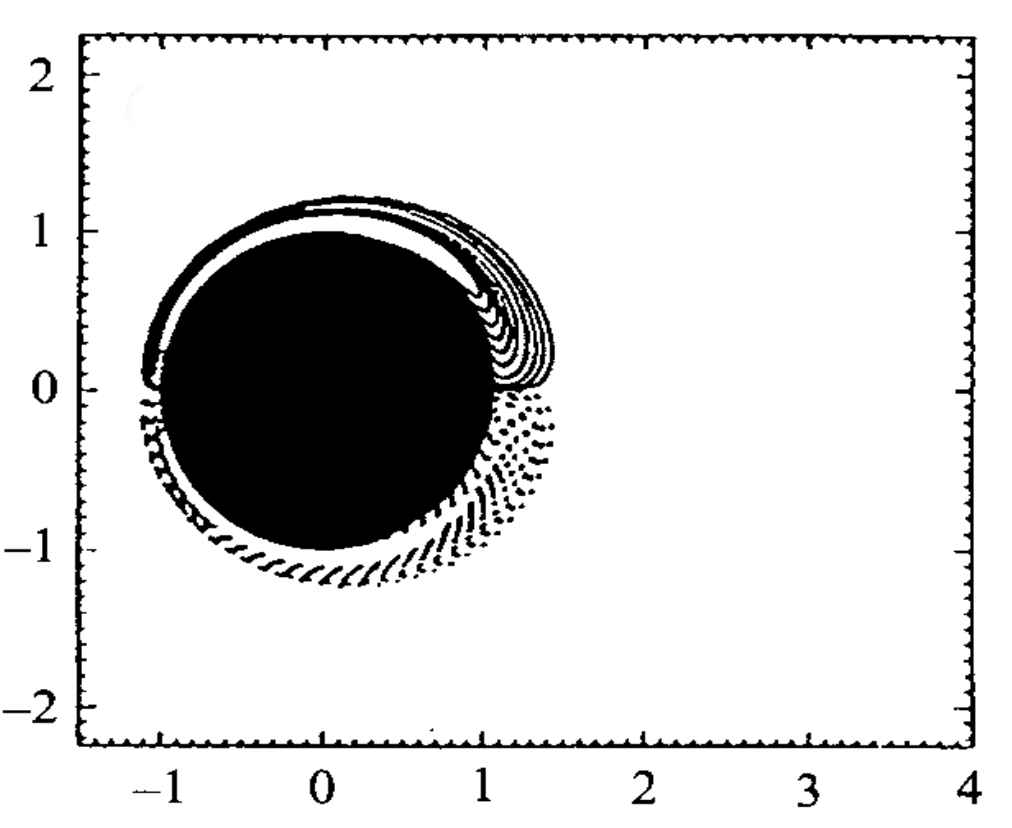
\includegraphics[height=0.2\textheight]{figures/eulerian/ISC_vorticityContours_t1_ref-mod.png}
             \caption{Reference: $T=1$}
             \label{fig:ISC_vorticityContours_t1_ref}
     \end{subfigure}%
     ~ %add desired spacing between images, e. g. ~, \quad, \qquad etc.
       %(or a blank line to force the subfigure onto a new line)
     \begin{subfigure}[t]{0.45\textwidth}
             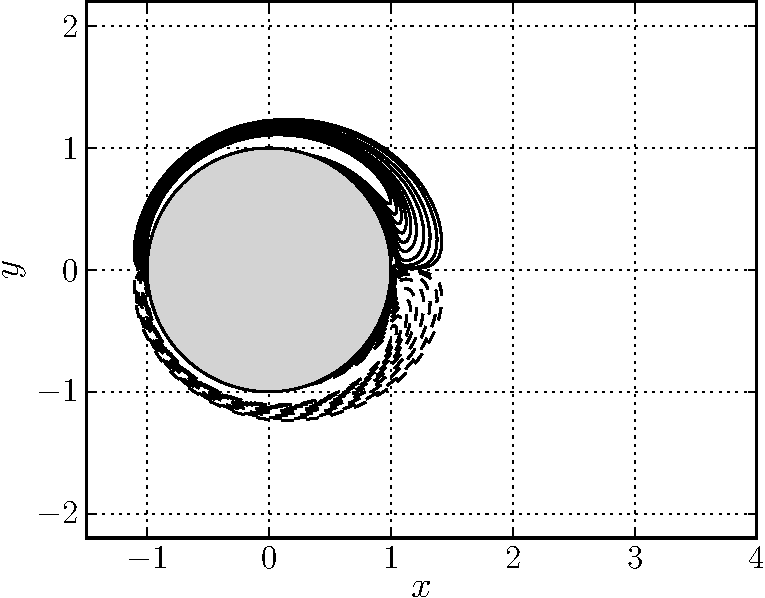
\includegraphics[height=0.2\textheight]{figures/eulerian/ISC_vorticityContours_t1_fliped-crop.pdf}
             \caption{Present: $T=1$}
             \label{fig:ISC_vorticityContours_t1-crop}
     \end{subfigure}
     
     \begin{subfigure}[t]{0.45\textwidth}
             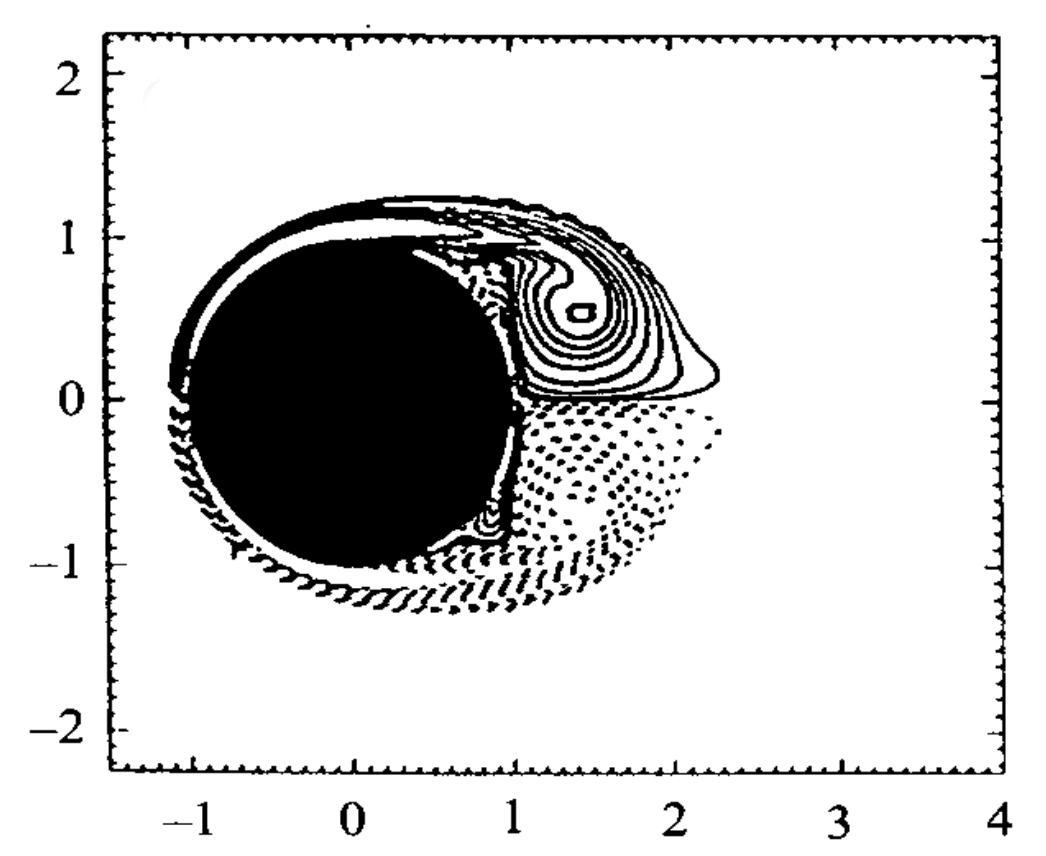
\includegraphics[height=0.2\textheight]{figures/eulerian/ISC_vorticityContours_t3_ref-mod.png}
             \caption{Reference: $T=3$}
             \label{fig:ISC_vorticityContours_t3_ref}
     \end{subfigure}%
     ~ %add desired spacing between images, e. g. ~, \quad, \qquad etc.
       %(or a blank line to force the subfigure onto a new line)
     \begin{subfigure}[t]{0.45\textwidth}
             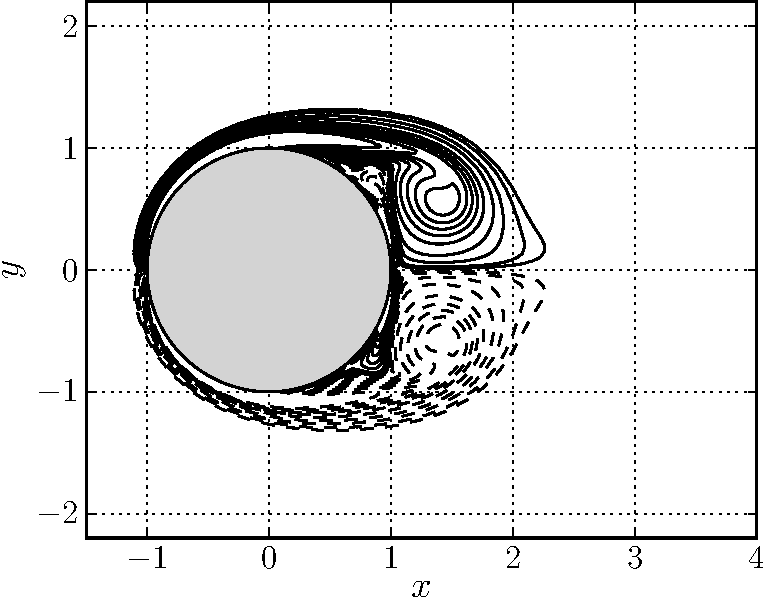
\includegraphics[height=0.2\textheight]{figures/eulerian/ISC_vorticityContours_t3_fliped-crop.pdf}
             \caption{Present: $T=3$}
             \label{fig:ISC_vorticityContours_t3-crop}
     \end{subfigure} 
     
     
     \begin{subfigure}[t]{0.45\textwidth}
             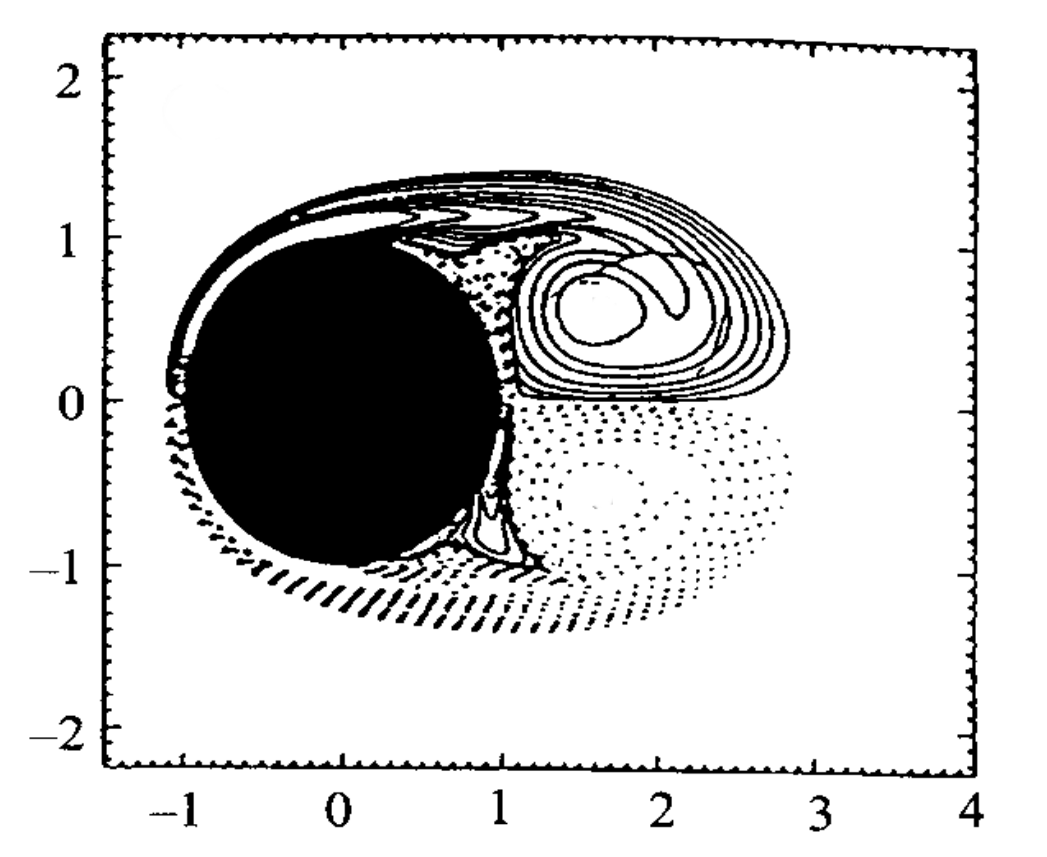
\includegraphics[height=0.2\textheight]{figures/eulerian/ISC_vorticityContours_t5_ref-mod.png}
             \caption{Reference: $T=5$}
             \label{fig:ISC_vorticityContours_t5_ref}
     \end{subfigure}%
     ~ %add desired spacing between images, e. g. ~, \quad, \qquad etc.
       %(or a blank line to force the subfigure onto a new line)
     \begin{subfigure}[t]{0.45\textwidth}
             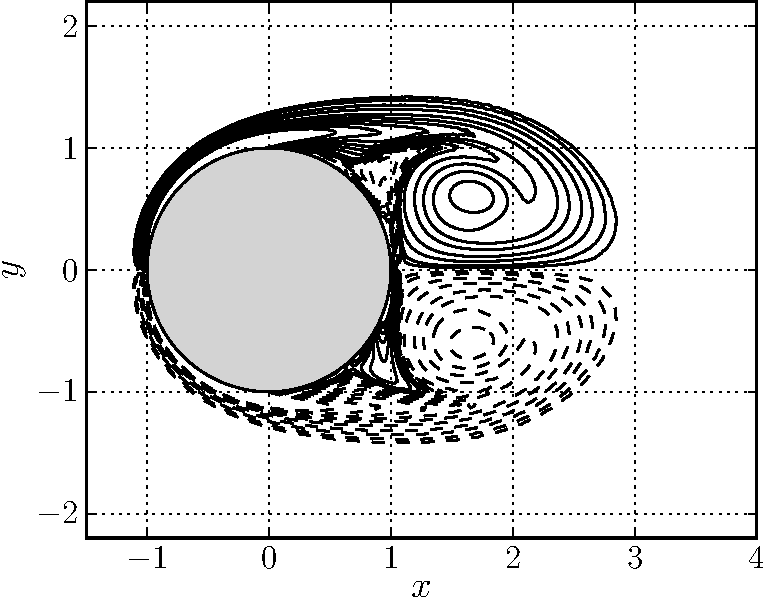
\includegraphics[height=0.2\textheight]{figures/eulerian/ISC_vorticityContours_t5_fliped-crop.pdf}
             \caption{Present: $T=5$}
             \label{fig:ISC_vorticityContours_t5-crop}
     \end{subfigure}
     
     \begin{subfigure}[t]{0.45\textwidth}
             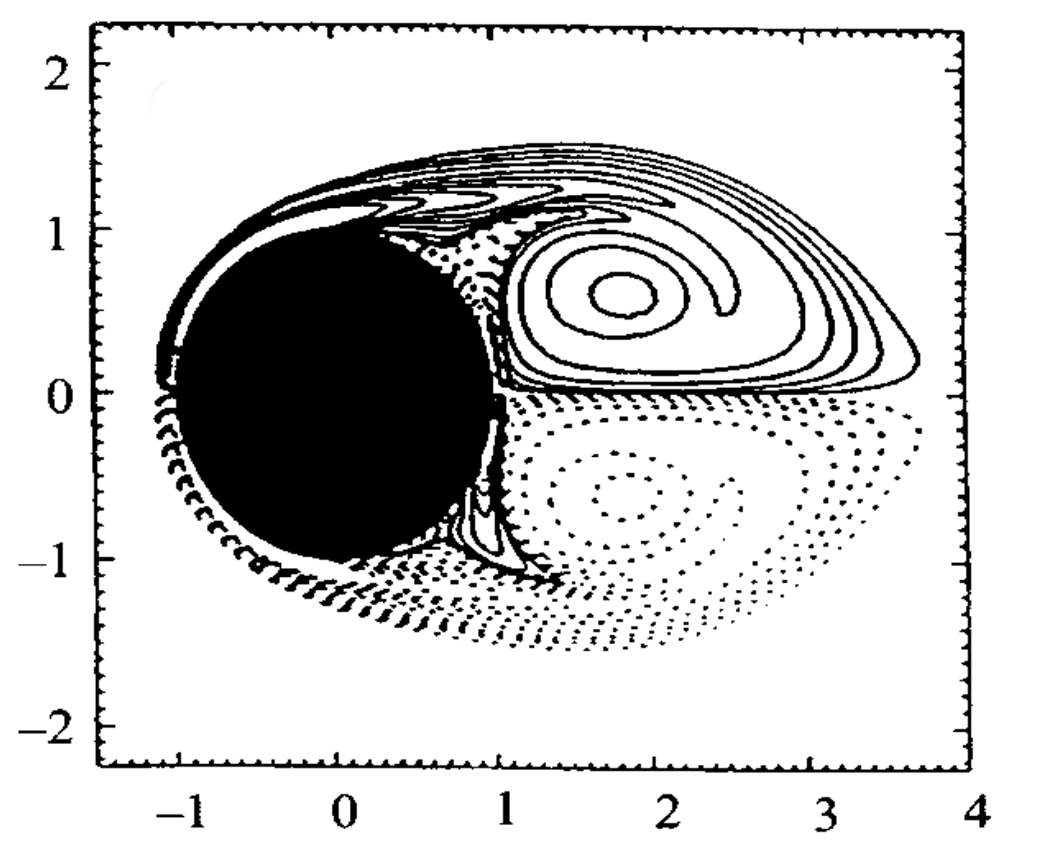
\includegraphics[height=0.2\textheight]{figures/eulerian/ISC_vorticityContours_t7_ref-mod.png}
             \caption{Reference: $T=7$}
             \label{fig:ISC_vorticityContours_t7_ref}
     \end{subfigure}%
     ~ %add desired spacing between images, e. g. ~, \quad, \qquad etc.
       %(or a blank line to force the subfigure onto a new line)
     \begin{subfigure}[t]{0.45\textwidth}
             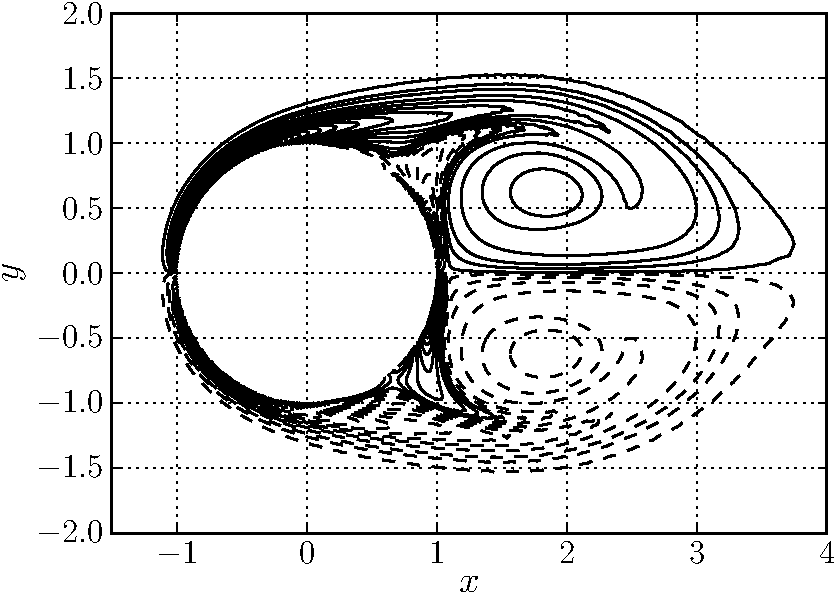
\includegraphics[height=0.2\textheight]{figures/eulerian/ISC_vorticityContours_t7_fliped-crop.pdf}
             \caption{Present: $T=7$}
             \label{fig:ISC_vorticityContours_t7-crop}
     \end{subfigure}         

     \caption{Comparison of the vorticity contours for $T=[1,3,5,7]$ with contour levels [$-7,...,-2,-1,-0.5,-0.2,-0.1,0.1,0.2,0.5,1,2,...,7$], showing negative vorticity (solid) and positive vorticity (dotted). The present study (right) is compared with plots obtained from Koumoutsakos and Leonard \cite{Koumoutsakos1995a} (left).}
     \label{fig:ISCS_vorticityContours_comparison}
	\end{figure}
	
	\begin{figure}[p]
	\centering
	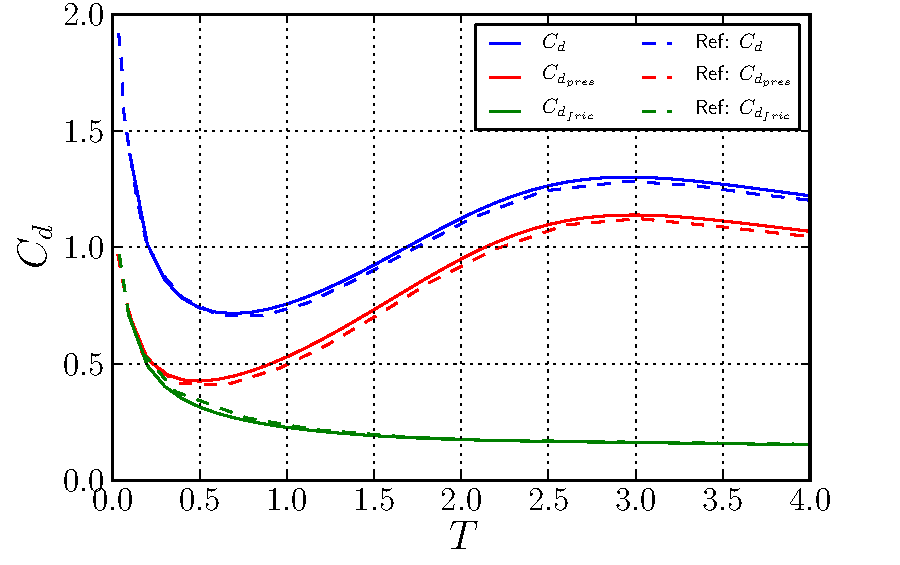
\includegraphics[width=0.7\linewidth]{./figures/eulerian/ISC_dragEvolution2.pdf}
	\caption{Evolution of drag force. The figure depicts the total drag coefficient $C_d$ [{\color{plotBlue}{---}}, solid blue], the pressure drag coefficient $C_{d_{\mathrm{pres}}}$ [{\color{plotRed}{---}}, solid red] and the friction drag coefficient $C_{d_{\mathrm{fric}}}$ [{\color{plotGreen}{---}}, solid green]. The dotted lines indicate the data obtained from literature, Koumoutsakos and Leonard \cite{Koumoutsakos1995a}.}
	\label{fig:ISC_dragEvolution}
	\end{figure}
	
	\begin{figure}[p]
	\centering
	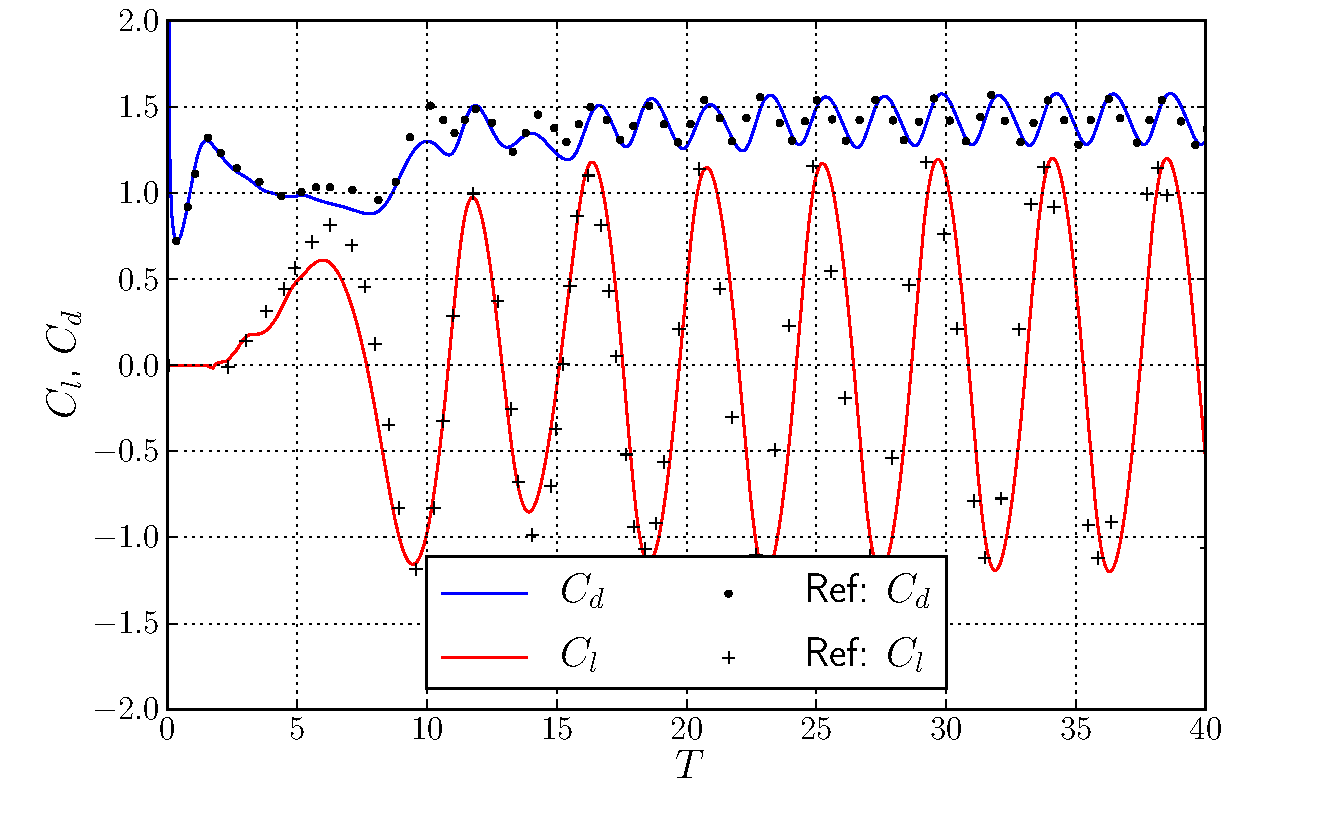
\includegraphics[width=0.7\linewidth]{./figures/eulerian/ISC_LongRun_dragLiftEvolution_fixed.pdf}
	\caption{Evolution of the lift coefficient $C_l$ and the drag coefficient $C_d$ from $T=0$ to $T=40$ with artificial perturbation \cite{Lecointe1984}. The dotted lines represent the data obtained from literature, Rosenfeld et al. \cite{MosheRosenFeldDochanKwak1991}.}
	\label{fig:ISC_LongRun_dragLiftEvolution}
	\end{figure}	

\subsubsection*{Results and Discussion}

Figure \ref{fig:ISCS_vorticityContours_comparison} depicts the evolution of the vorticity at $T=[1,3,5,7]$. The iso-vorticity contours of the present study are compared with the reference data obtained from Koumoutsakos and Leonard \cite{Koumoutsakos1995a}. At $T=1$, negative and positive vorticity is generated at the top and bottom of the cylinder, respectively. This results from satisfying the no-slip boundary condition. As time progresses, two primary vortices are formed behind the cylinder, increasing in shape as time advances. Comparing the vorticity contours, we can say that the contour lines match with the literature. 

Using equations \ref{eq:LiftDragEq} to \ref{eq:LiftDragCoeffEq}, we were able to calculate the lift and the drag force acting on the cylinder as time progresses, which we used to validate against the literature. Figure \ref{fig:ISC_dragEvolution} shows the components of the drag force (friction drag $C_{d_{\mathrm{fric}}}$, pressure drag $C_{d_{\mathrm{pres}}}$) acting on the surface of the body. At $T=0$, we have a singularity in the total drag $C_d$ acting on the body due to the impulsive start of the flow. It then plunges to $C_d=0.75$ at $T=0.8$ and peaks again near $T=3$ with $C_d=1.3$. The dotted line is the data obtained from literature \cite{Koumoutsakos1995a} and we see that the results of the simulation match well with the literature.

A final comparison was done for the evolution of the lift and the drag coefficients for a larger period ($T=0$ to $T=40$), which was used to determine the oscillatory behavior of the forces. For lower Reynolds number, the vorticity field is symmetric across the $x$-axis for a long time. This meant that the oscillatory behavior of the forces starts at a much later time. Therefore, we prescribed an artificial perturbation to the problem to create an asymmetry in the vorticity field which trips the wake. The perturbation was performed according to Leocointe and Piquet \cite{Lecointe1984},
	\begin{equation}
	 u_{\mathrm{wall}} = \begin{cases}
	 0.15 & 3 \leqslant T \leqslant 3.5, \\
	 -0.25 & 3.5 \leqslant T \leqslant 5.
	 \end{cases}
	\label{eq:perturbation}
	\end{equation}
	
With this, we could ensure that we have a controlled behavior for the lift and drag, which we used to determine the amplitude and the frequency of the oscillation. Figure \ref{fig:ISC_LongRun_dragLiftEvolution} compares the evolution of the lift and drag for $T=0$ to $T=40$. We see that our numerical scheme performs very similar to the literature \cite{MosheRosenFeldDochanKwak1991}. However, there is a slight difference, which is due to the under-resolution of the Eulerian domain downstream of the cylinder, making the wake our Eulerian method more dissipative than the Lagrangian reference method used by Koumoutsakos and Leonard \cite{Koumoutsakos1995a}.

\section{Summary}

In summary, we have investigated the Eulerian domain of our hybrid method in this chapter. The Eulerian method was used to resolve the near-body region where generation of vorticity from the \textit{no-slip} boundary was of concern. The advantage of an Eulerian formulation is that it is much more efficient in resolving the boundary layer than the VPM described in chapter \ref{ch:lagrangian}. We decided to use a \printAcron{Finite Element Method}{FEM} to solve the incompressible laminar Navier-Stokes problem of the near-wall region.

In section \ref{sec:e-ithfem}, an introduced to the FEM was given. We investigated the theory of finite element discretization, and introduced the concept of functions and function spaces of a finite elements. Finally, we introduced the variational formulation for solving the PDE.

In section \ref{sec:e-stfep}, we introduced \fenics project, a collaborative work of various universities that developed tools to perform automated finite element algorithms. The \dolfin library of \fenics project provided the finite element library for set up and solve the finite element problem. We used the \dolfin library wrapped in \python. It uses automated code generation thus maintaining high-level mathematic expressions but still provided an efficient, a multi-threaded performance. \gmsh mesh generation tool was used to generate the unstructured mesh of the fluid domain.

In section \ref{sec:e-sinse}, we investigated the \printAcron{Incremental Pressure Correction Scheme}{IPCS} for solving the incompressible Navier-Stokes equations. The scheme allows us to decouple the velocity $\mathbf{u}$ and pressure $p$ from the momentum equation. Furthermore, we determined an approach for solving the vorticity field, which was computationally efficient.

In section \ref{sec:eu-voem}, we verified and validated our implementation of the Eulerian method. A Lamb-Oseen Vortex test case was used to verify the implementation of the Eulerian method, and concluded that the method had a $1^{\mathrm{st}}$-order convergence in time and $2^{\mathrm{nd}}$-order convergence in space. To validate the calculation of vorticity and the vorticity production of the no-slip boundary, we used the high-fidelity numerical test case of Clercx and Bruneau \cite{Clercx2006a}. The literature studied the collision of dipole with the wall, investigating the change in kinetic energy $E$, enstrophy $\Omega$, and Palinstrophy $P$ over time. Furthermore, we compared the generation of vorticity at the boundary, validating a consistent result. 

The final test case involved simulating an impulsively started cylinder at $Re=550$. We investigated the shedding of vorticity in time progress and observed that it matched the reference data provided by Koumoutsakos and Leonard \cite{Koumoutsakos1995a}. We also investigated the long term evolution of the lift and drag of the cylinder, and observed that the frequency and the amplitude of the oscillation was similar to literature study of Rosenfeld et al. \cite{MosheRosenFeldDochanKwak1991}.

%

%	\begin{itemize}
%	\item The Eulerian method is used to highly resolve the near-body region of the fluid.
%	\item We have used a Finite Element method to solve the incompressible laminar Navier-Stokes problem using the velocity-pressure $\mathbf{u}-p$ formulation.
%	\item \printAcron{Incremental Pressure Correction Scheme}{IPCS} was used to solve the Navier-Stokes problem, allowing us to decouple the velocity $\mathbf{u}$ and pressure $p$ from the momentum equation.
%	\item \dolfin library from the \fenics project was used to perform automated finite element algorithms for solving the partial different equations.
%	\item \gmsh mesh generation tool was used to generate the unstructured mesh of the fluid domain.
%	\item Once we have determined the velocity $\mathbf{u}$ and the pressure $p$ fields, we can determine the vorticity associated to the fluid using an optimized calculation algorithm.
%	\item A Lamb-Oseen Vortex test case was used to verify the implementation of the Eulerian method, and concluded that the method had a $1^{\mathbf{st}}$-order convergence in time and $2^{\mathrm{nd}}$-order convergence in space.
%	\item To validate the vorticity handling and the vorticity production of the no-slip boundary, we used the high-fidelity numerical test case of Clercx \& Bruneau investigation the collision of dipole with the wall at $Re=625$. Investigating the change in kinetic energy $E$, enstrophy $\Omega$, and Palinstrophy $P$, we validate that the results matched the literature. We evaluated the vorticity generated at boundary, which also showed that our numerical method handels according to theory.
%	\item The final test case involved simulating an impulsively started cylinder at $Re=550$. We investigated the shed of vorticity at time progress and validated that it matched the reference data provided by Koumoutsakos \& ???. Finally, we investigated the evolution of the lift and drag of the cylinder, and we saw that the frequency and the amplitude of the oscillation matched the theory. Therefore, our Eulerian method accurate determine the fluid behavior past an object such as the Strouhal number St.
%	\end{itemize}

%\subsection*{Eulerian method algorithm}
%
%The algorithm for the Eulerian method can be summarized as follows:
%
%	\begin{enumerate}
%	\item \textbf{Mesh generation}: We generate the mesh of the fluid domain using \gmsh before the iteration.
%	\item \textbf{Determine the boundary condition}: We need to determine the boundary conditions for the boundary domains: $\partial \Omega_{\mathrm{wall}}$, $\partial \Omega_{\mathrm{dirichlet}}$, $\partial \Omega_{\mathrm{pressure}}$. If we have dirichlet velocity boundary conditions for all the exterior boundaries, we do not have to apply any pressure boundary conditions at $\partial \Omega_{\mathrm{pressure}}$.
%	\item \textbf{Solve the IPCS}: Using IPCS, time march from $t_n$ to $t_{n+1}$ to solve for the new velocity $\mathbf{u}$ and pressure $p$ field.
%	\item \textbf{Determine the vorticity}: Using the algorithm described in \ref{??}, solve for the vorticity field $\omega$ at the time $t_{n+1}$. 
%	\end{enumerate}
%
%Once we have the well-resolved vorticity $\omega$ of the near-body region, we use it to couple it with the Lagrangian method with our Hybrid coupling scheme.

\section{Chapter Nomenclature}

{\textbf{\textsf{Latin Symbols}}}

{\renewcommand{\arraystretch}{1.2} %<- modify value to suit your needs
\begin{longtable}{p{1.5cm}p{10.5cm}p{1.5cm}}
	
	$\mathbf{A}$ & Coefficient matrix & - \\
	$b$ & Right-Hand-Side & - \\
	$c $ & Reference length (chord) & \si{m}\\
	$C_d$ & Drag coefficient & -\\
	$C_l$ & Lift coefficient & -\\
	$\mathrm{CFL}$ & CFL number & -\\
	
	
	$\hat{\mathbf{e}}$ & Cartesian unit vector & -\\
	$E$ & Kinetic Energy & \si{J} \\

	$f$ & Source terms & -\\
	
	$\mathbf{I}$ & Identity matrix & -\\

	$\hat{\mathbf{n}}$ & Unit normal vector & -\\

	$N_{cells}$ & Number of FE mesh cells & -\\	
	$N_t$ & Number of time integration steps & - \\

	$p$ & \vtop{\hbox{\strut Pressure}\hbox{\strut Trial function for pressure}} & \vtop{\hbox{\strut \si{Pa}}\hbox{\strut -}}\\
	
	$\mathcal{P}$ & Lagrange polynomial & -\\

	$q$ & \vtop{\hbox{\strut Degree of Lagrange polynomial $\mathcal{P}_q$}\hbox{\strut Test function for pressure}} & \vtop{\hbox{\strut - }\hbox{\strut -}}\\
	 %$q$ & Degree of Lagrange polynomial $\mathcal{P}_q$; Test function for pressure & -\\
	 
	 $Q$ & Scalar-valued function space for pressure $p$& -\\	
	$Re$ & Reynolds number & - \\
	 $t_n$ & Simulation time at $n^{\mathrm{th}}$ step & \si{s}\\	
	
	$\mathcal{T}_h$ & Finite Element mesh & -\\

 	$T$ & Cell of Finite Element mesh & -\\	
 	
 	$\mathbf{u}$ & \vtop{\hbox{\strut Velocity }\hbox{\strut Trial function for velocity}} & \vtop{\hbox{\strut \si{m.s^{-1}} }\hbox{\strut - }}\\
 	
 	$\mathbf{u}^{\star}$ & Tentative velocity & \si{m.s^{-1}}\\
 		
 	$v$ & Test function for velocity& -\\				
 	$V$ & Trial vector function space for velocity& - \\
 	$\hat{V}$ & Test vector function space for velocity& -\\
 

	 $w$ & Trial function for vorticity & -\\
	 
	 $x$ & Test function for vorticity & -\\
	 $X$ & Scalar-valued function space for vorticity $\omega$ & -\\
\end{longtable}}

{\textbf{\textsf{Greek Symbols}}}

{\renewcommand{\arraystretch}{1.2} %<- modify value to suit your needs
\begin{longtable}{p{1.5cm}p{10.5cm}p{1.5cm}}

	$\Gamma$ & Circulation & \si{m^{2}.s^{-1}}\\
	$\Delta h$ & Mesh cell size & \si{m} \\
	$\Delta t_E$ & Eulerian time step size & \si{s} \\
	
	$\epsilon$ & Symmetric gradient & -\\
	
	$\nu$ & Kinematic viscosity & \si{kg.s^{-1}.m^{-1}}\\


	$\rho$ & Fluid density & \si{kg.m^{-3}}\\

	$\sigma$ & Cauchy stress tensor & \si{Pa}\\
	$\Sigma_d$ & Dirichlet velocity boundary & - \\
	$\Sigma_{p}$ & Pressure outlet boundary & - \\
	$\Sigma_{w}$ & No-slip wall boundary & - \\

	$\psi$ & Basis function & - \\
	$\psi$ & Basis function & -\\

	$\omega$ & Vorticity & \si{s^{-1}}\\
	$\Omega$ & Fluid domain & -\\	
	$\Omega_E$ & Eulerian fluid domain & -\\	
	%$\Omega_L$ & Lagrangian fluid domain & -\\
	$\partial \Omega$ & Boundary of the domain $\Omega$ & -\\

	
\end{longtable}}
					
